%%%%%%%%%%%%%%%%%%%%%%%%%%%%%%%%%%%%%%%%%%%%%%%%%%%%%%%%%%%%%%%%%%%%%%
% Overleaf (WriteLaTeX) Example: Molecular Chemistry Presentation
%
% Source: http://www.overleaf.com
%
% In these slides we show how Overleaf can be used with standard 
% chemistry packages to easily create professional presentations.
% 
% Feel free to distribute this example, but please keep the referral
% to overleaf.com
% 
%%%%%%%%%%%%%%%%%%%%%%%%%%%%%%%%%%%%%%%%%%%%%%%%%%%%%%%%%%%%%%%%%%%%%%

\documentclass{beamer}

\mode<presentation>
{
  \usetheme{Madrid}       % or try default, Darmstadt, Warsaw, ...
  \usecolortheme{default} % or try albatross, beaver, crane, ...
  \usefonttheme{default}    % or try default, structurebold, ...
  \setbeamertemplate{navigation symbols}{}
  \setbeamertemplate{caption}[numbered]
} 

\usepackage[english]{babel}
\usepackage[utf8x]{inputenc}
\usepackage{chemfig}
\usepackage[version=3]{mhchem}

\usepackage{hyperref}
  \hypersetup{colorlinks=true}
  \hypersetup{urlcolor=blue}
  \hypersetup{linkcolor = .}
\usepackage{xcolor}
\usepackage{siunitx}
  \sisetup{separate-uncertainty = true}
\usepackage{physics}
\usepackage[font=small,labelfont=bf]{caption}
\usepackage{subcaption}
\usepackage[en-GB]{datetime2}
\usepackage{feynmp}
\DeclareGraphicsRule{*}{mps}{*}{}

\usepackage{scalerel}
\newcommand{\mylbrace}[2]{\vspace{#2pt}\hspace{6pt}\scaleleftright[\dimexpr5pt+#1\dimexpr0.06pt]{\lbrace}{\rule[\dimexpr2pt-#1\dimexpr0.5pt]{-4pt}{#1pt}}{.}}
\newcommand{\myrbrace}[2]{\vspace{#2pt}\scaleleftright[\dimexpr5pt+#1\dimexpr0.06pt]{.}{\rule[\dimexpr2pt-#1\dimexpr0.5pt]{-4pt}{#1pt}}{\rbrace}\hspace{6pt}}

% Here's where the presentation starts, with the info for the title slide
\title[$B^\pm\to(K^+K^-\pi^+\pi^-)_DK^\pm$]{Binning scheme for \texorpdfstring{$\gamma$}{gamma} measurement in \texorpdfstring{$B^\pm\to(K^+K^-\pi^+\pi^-)_DK^\pm$}{B to K+K-pi+pi-} decays}
\author{Martin Tat}
\institute{Oxford LHCb}
\date{\today}

\titlegraphic{
\includegraphics[width = 4cm]{lhcb.jpg}\hspace{3cm}~%
              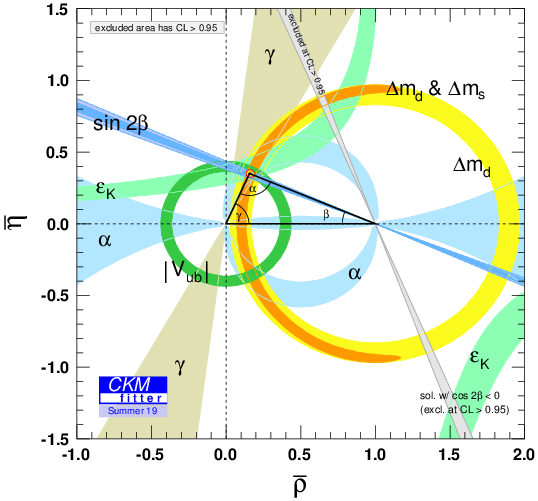
\includegraphics[width = 3cm]{ckmfitter.png}}

\begin{document}

\begin{frame}
  \titlepage
\end{frame}

% These three lines create an automatically generated table of contents.
\begin{frame}{Outline}
  \tableofcontents
\end{frame}

\section{Current progress}
\begin{frame}{Current progress}
  \begin{itemize}
    \item{Events generated in AmpGen using amplitude model \href{https://arxiv.org/abs/1811.08304}{arXiv:1811.08304}}
    \begin{itemize}
      \item{Assumed event yield: $2000$ ($1000$ $B^+$, $1000$ $B^-$)}
      \item{Assumed parameters in toy model: $\gamma = 75^\circ$, $\delta_B = 130^\circ$, $r_B = 0.1$}
    \end{itemize}
    \item{Unbinned fit using SimFit in AmpGen}
    \item{Binned fit and pull studies}
    \item{Develop suitable binning scheme}
  \end{itemize}
\end{frame}

\section{Unbinned fit}
\begin{frame}{Unbinned fit with amplitude model}
  \vspace{-0.3cm}
  \begin{align*}
    \mathcal{A}(B^-\to(K^+K^-\pi^+\pi^-)_DK^-) =& \mathcal{A}_B\mathcal{A}(D^0\to K^+K^-\pi^+\pi^-) \\
  +& \mathcal{A}_B\mathcal{A}(\bar{D^0}\to K^+K^-\pi^+\pi^-)r_Be^{i(\delta_B - \gamma)}
  \end{align*}
  \vspace{-0.5cm}
  \begin{itemize}
    \item{$\mathcal{A}(D\to K^+K^-\pi^+\pi^-)$ obtained from amplitude model}
    \item{Fit with $\gamma$, $\delta_B$ and $r_B$ as free parameters}
    \item{Results from unbinned fit of $\SI{2e3}{}$ events:}
    \begin{itemize}
      \item{$\gamma = \SI{69(11)}{\degree}$}
      \item{$\delta_B = \SI{115(11)}{\degree}$}
      \item{$r_B = \SI{0.098(17)}{}$}
    \end{itemize}
    \item{Pulls of $\gamma$, $\delta_B$ and $r_B$ all have mean $0$ and std $1$ (see backup slides)}
  \end{itemize}
\end{frame}

\begin{frame}{Unbinned fit of $\SI{2e3}{}$ events with amplitude model}
  \begin{figure}
    \centering
    \vspace{-0.2cm}
    \begin{subfigure}{0.46\textwidth}
      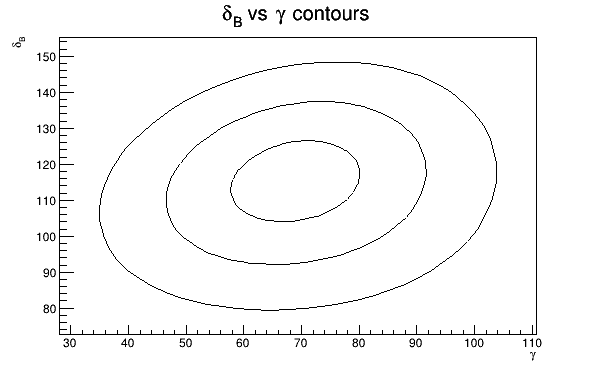
\includegraphics[width = 1.0\textwidth]{Contour_dB_vs_gamma_1K.png}
      \caption{$\gamma$ vs $\delta_B$}
    \end{subfigure}%
    \begin{subfigure}{0.46\textwidth}
      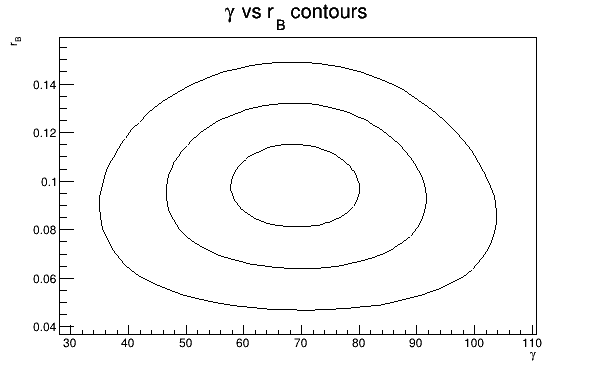
\includegraphics[width = 1.0\textwidth]{Contour_gamma_vs_rB_1K.png}
      \caption{$\gamma$ vs $r_B$}
    \end{subfigure}
    \begin{subfigure}{0.46\textwidth}
      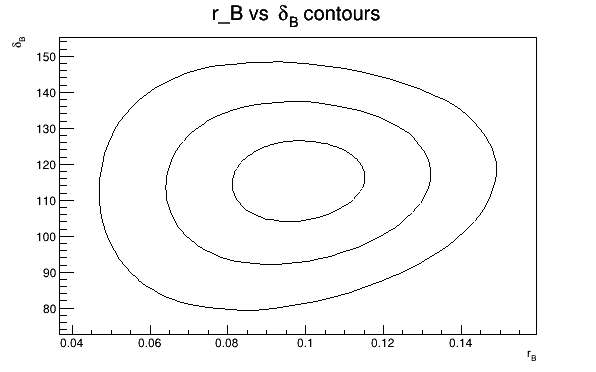
\includegraphics[width = 1.0\textwidth]{Contour_rB_vs_dB_1K.png}
      \caption{$r_B$ vs $\delta_B$}
    \end{subfigure}
  \end{figure}
\end{frame}

\section{Binned fit and pull studies}
\begin{frame}{Binned fit of $D\to K^+K^-\pi^+\pi^-$}
  \vspace{-0.5cm}
  \begin{align*}
    \mathcal{A}(B^-\to(K^+K^-\pi^+\pi^-)_DK^-) =& \mathcal{A}_B\mathcal{A}(D^0\to K^+K^-\pi^+\pi^-) \\
  +& \mathcal{A}_B\mathcal{A}(\bar{D^0}\to K^+K^-\pi^+\pi^-)r_Be^{i(\delta_B - \gamma)}
  \end{align*}
  \vspace{-0.5cm}
  \begin{block}{Event yield in bin $i$}
    $N^-_i = h_{B^-}\Big(K_i + \big(x_-^2 + y_-^2\big)\bar{K_i} + 2\sqrt{K_i\bar{K_i}}\big(x_-c_i + y_-s_i\big)\Big)$
    $N^+_i = h_{B^+}\Big(\bar{K_i} + \big(x_+^2 + y_+^2\big)K_i + 2\sqrt{K_i\bar{K_i}}\big(x_+c_i - y_+s_i\big)\Big)$
  \end{block}
  \begin{block}{CP-violating observables}
    $x_\pm = r_B\cos(\delta_B\pm\gamma), \quad y_\pm = r_B\sin(\delta_B\pm\gamma)$
  \end{block}
\end{frame}

\begin{frame}{Pull studies}
  \begin{itemize}
    \item{Used an arbitrary and naive binning scheme with $4$ bins}
    \item{$x_\pm$ pulls show asymmetric tails for $\SI{2e3}{}$ events}
    \item{Pulls for $\gamma$, $\delta_B$, $r_B$ are rubbish}
  \end{itemize}
  \begin{block}{Naive binning scheme}
    Split phase space along the boundaries $E_{K^+} = E_{K_-}$ and $E_{\pi^+} = E_{\pi^-}$ \\
    Bin $1$: $E_{K^+} > E_{K^-}, \quad E_{\pi^+} > E_{\pi^-}$, \dots
  \end{block}
  \begin{block}{$D$ decay hadronic parameters}
    \begin{equation*}
      c_i = \frac{\int_i\dd{\Phi}|\mathcal{A}(D^0)||\mathcal{A}(\bar{D^0})|\cos(\delta_D)}{\sqrt{\int_i\dd{\Phi}\abs{\mathcal{A}(D^0)}^2\int_i\dd{\Phi}\abs{\mathcal{A}(\bar{D^0})}^2}}, \quad K_i = \frac{\int_i\dd{\Phi}|\mathcal{A}(D^0)|^2}{\sum_j\int_j\dd{\Phi}\abs{\mathcal{A}(D^0)}^2}
    \end{equation*}
  \end{block}
\end{frame}

\begin{frame}{Pull study with $\SI{2e3}{}$ events}
  \begin{figure}
    \centering
    \vspace{-0.2cm}
    \begin{subfigure}{0.5\textwidth}
      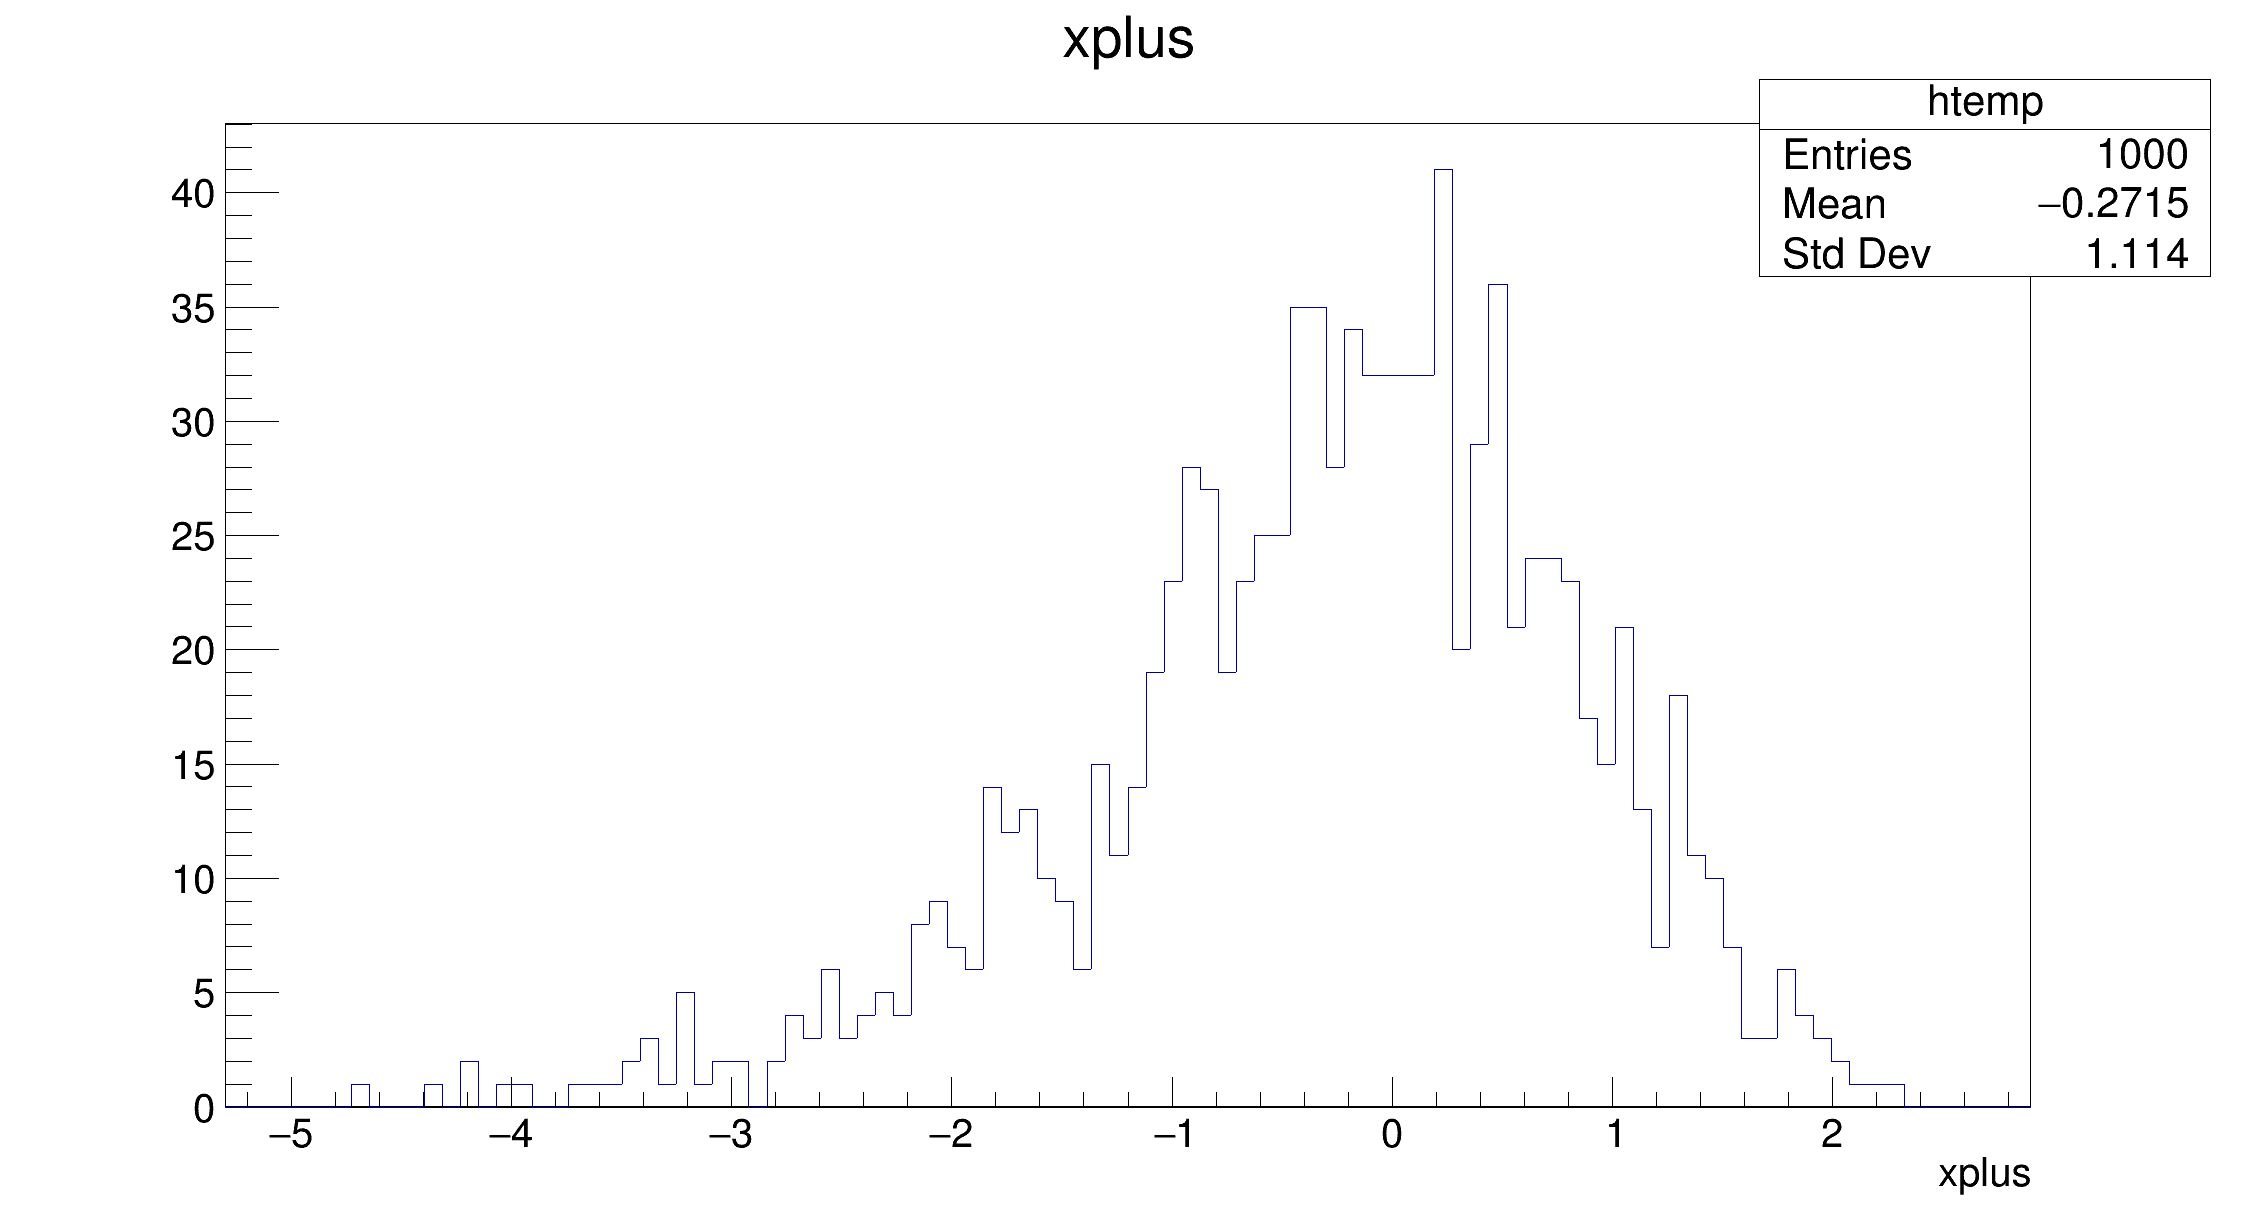
\includegraphics[width = 1.0\textwidth]{NaivePulls/xplus1K1K.png}
      \caption{$x_+$ pull}
    \end{subfigure}%
    \begin{subfigure}{0.5\textwidth}
      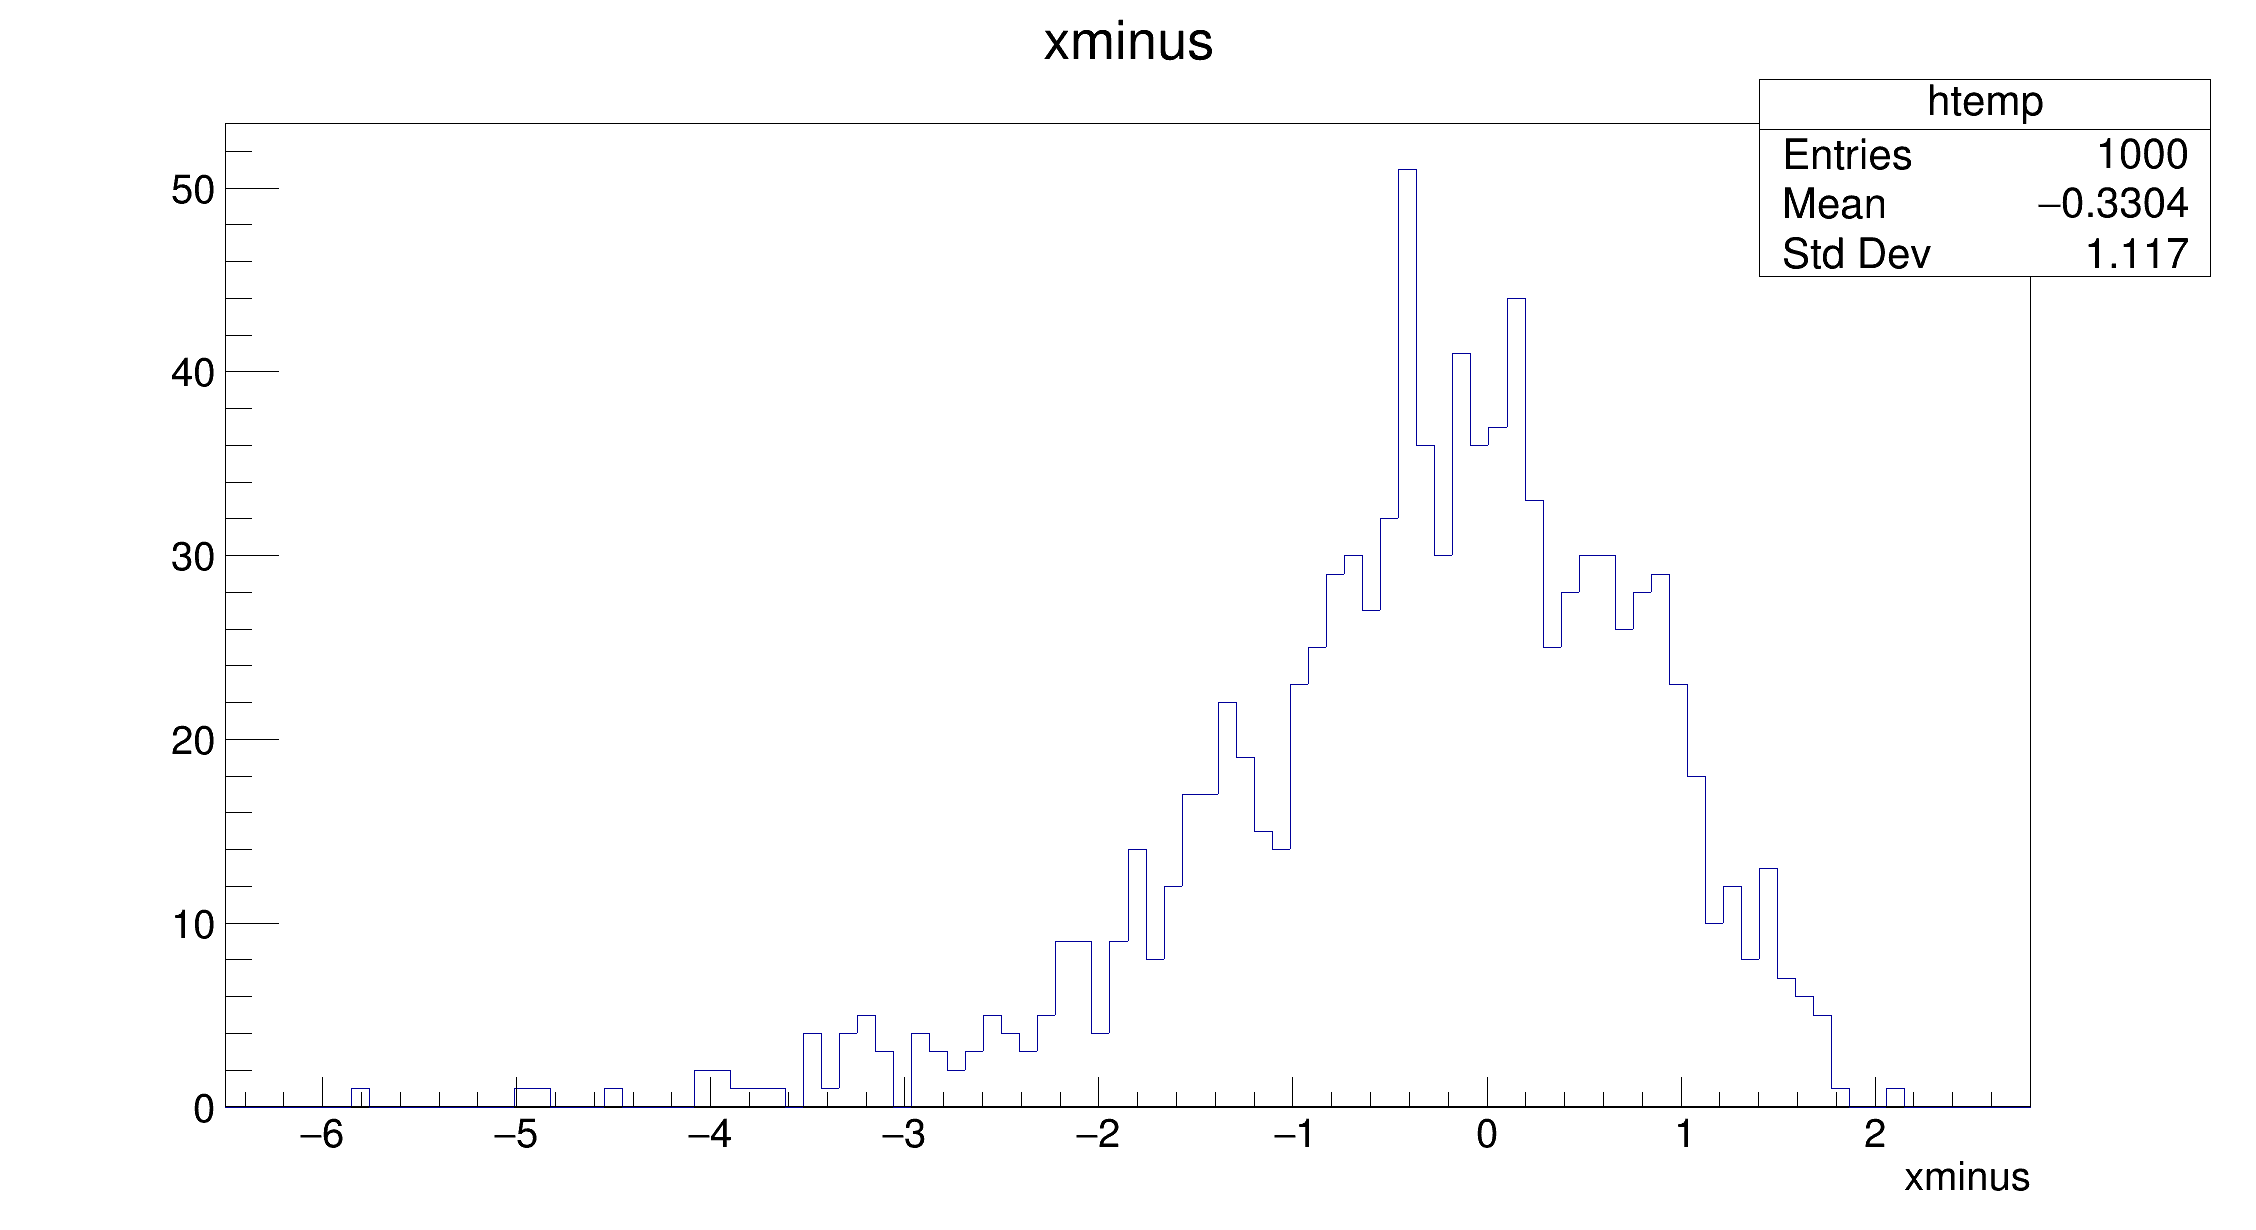
\includegraphics[width = 1.0\textwidth]{NaivePulls/xminus1K1K.png}
      \caption{$x_-$ pull}
    \end{subfigure}
    \begin{subfigure}{0.5\textwidth}
      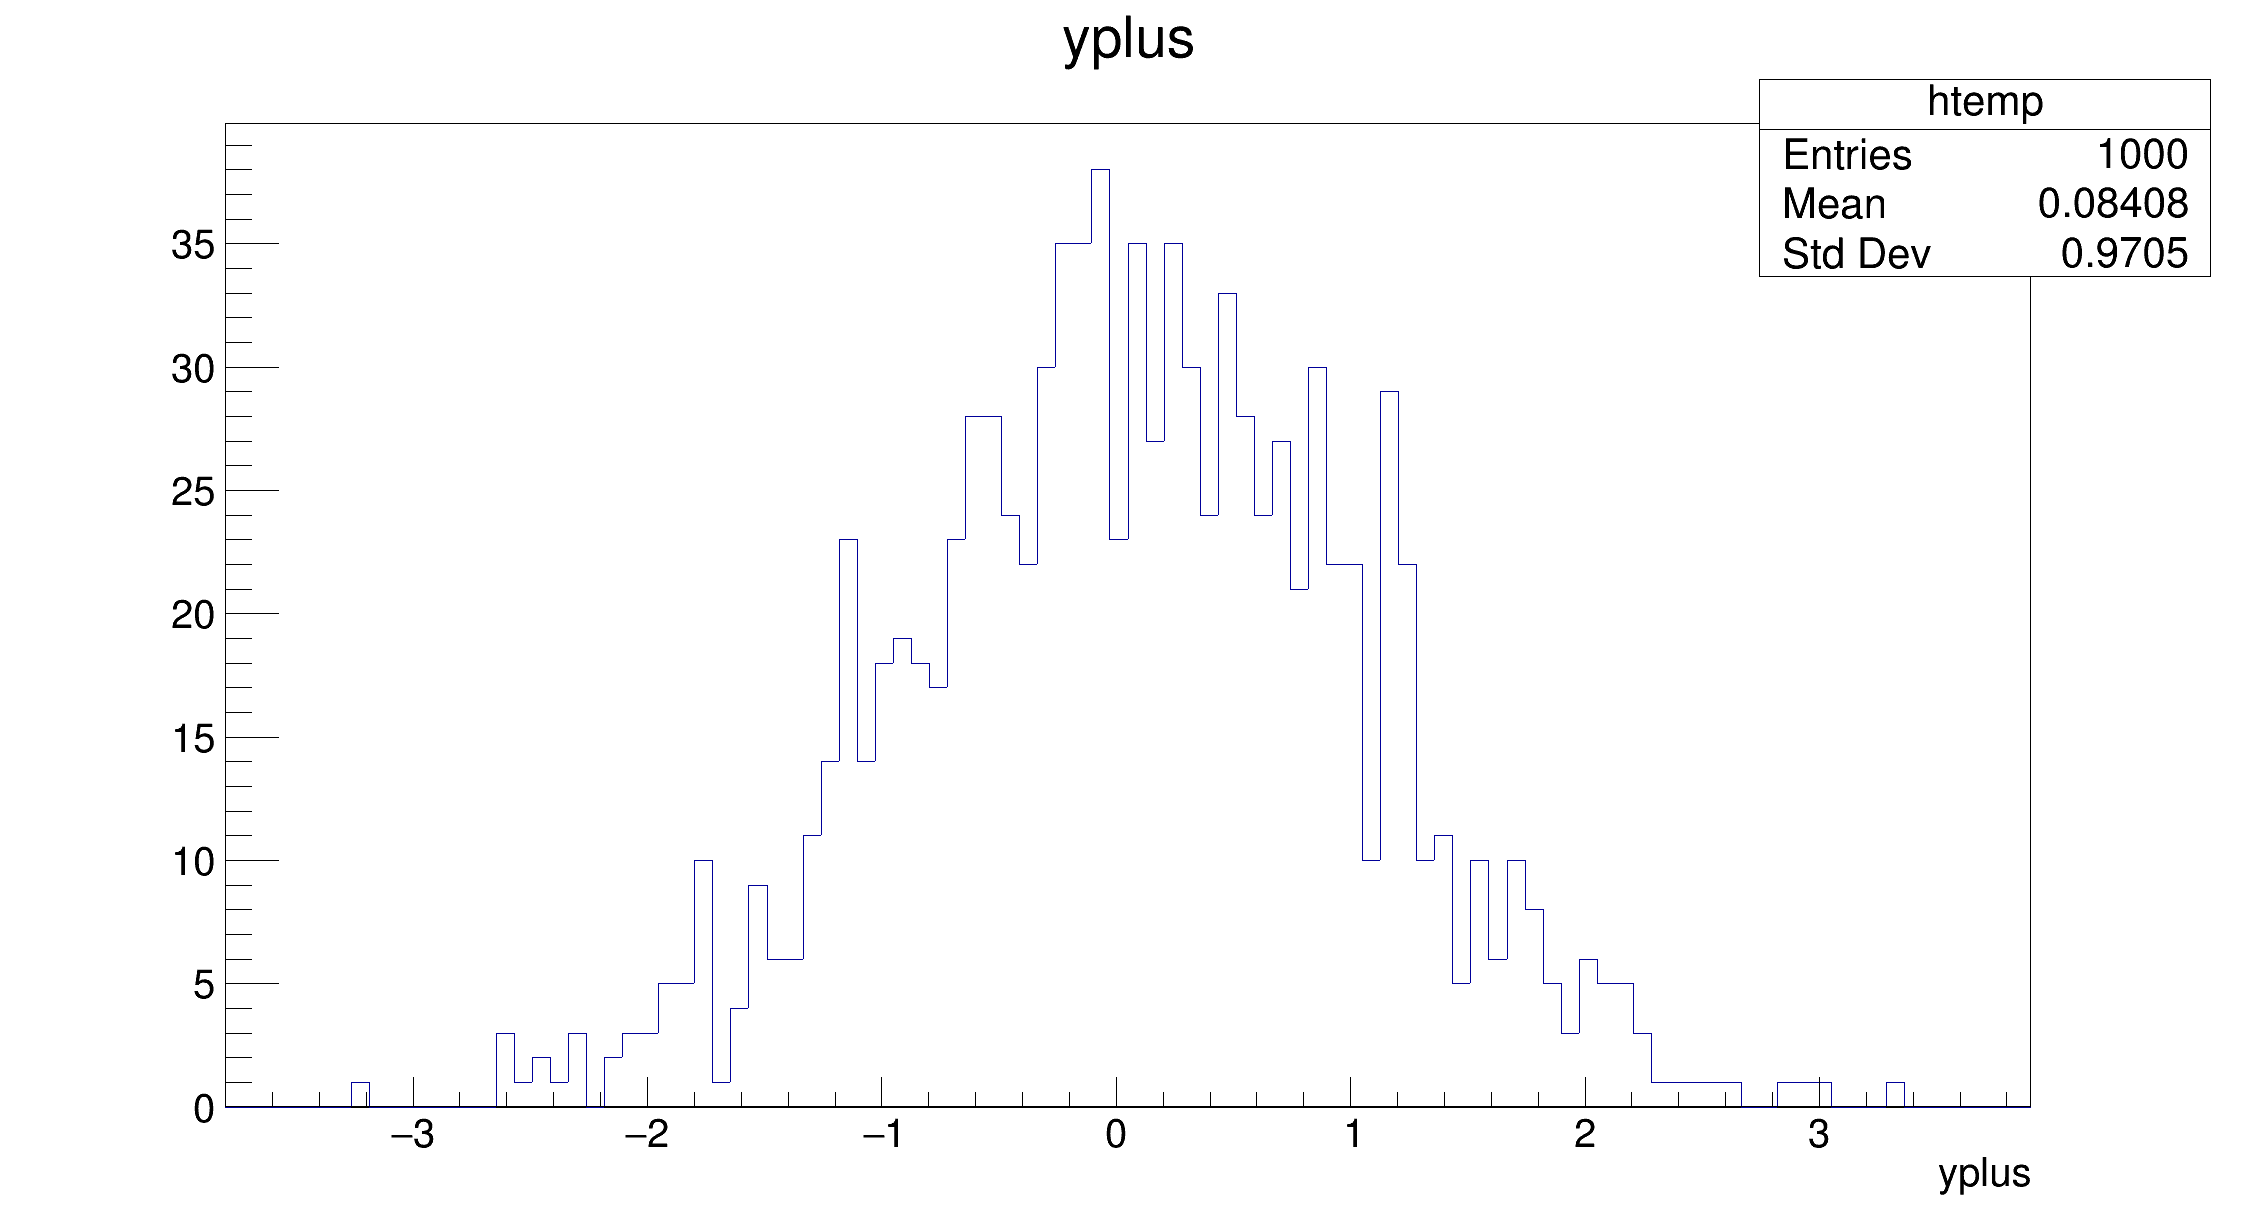
\includegraphics[width = 1.0\textwidth]{NaivePulls/yplus1K1K.png}
      \caption{$y_+$ pull}
    \end{subfigure}%
    \begin{subfigure}{0.5\textwidth}
      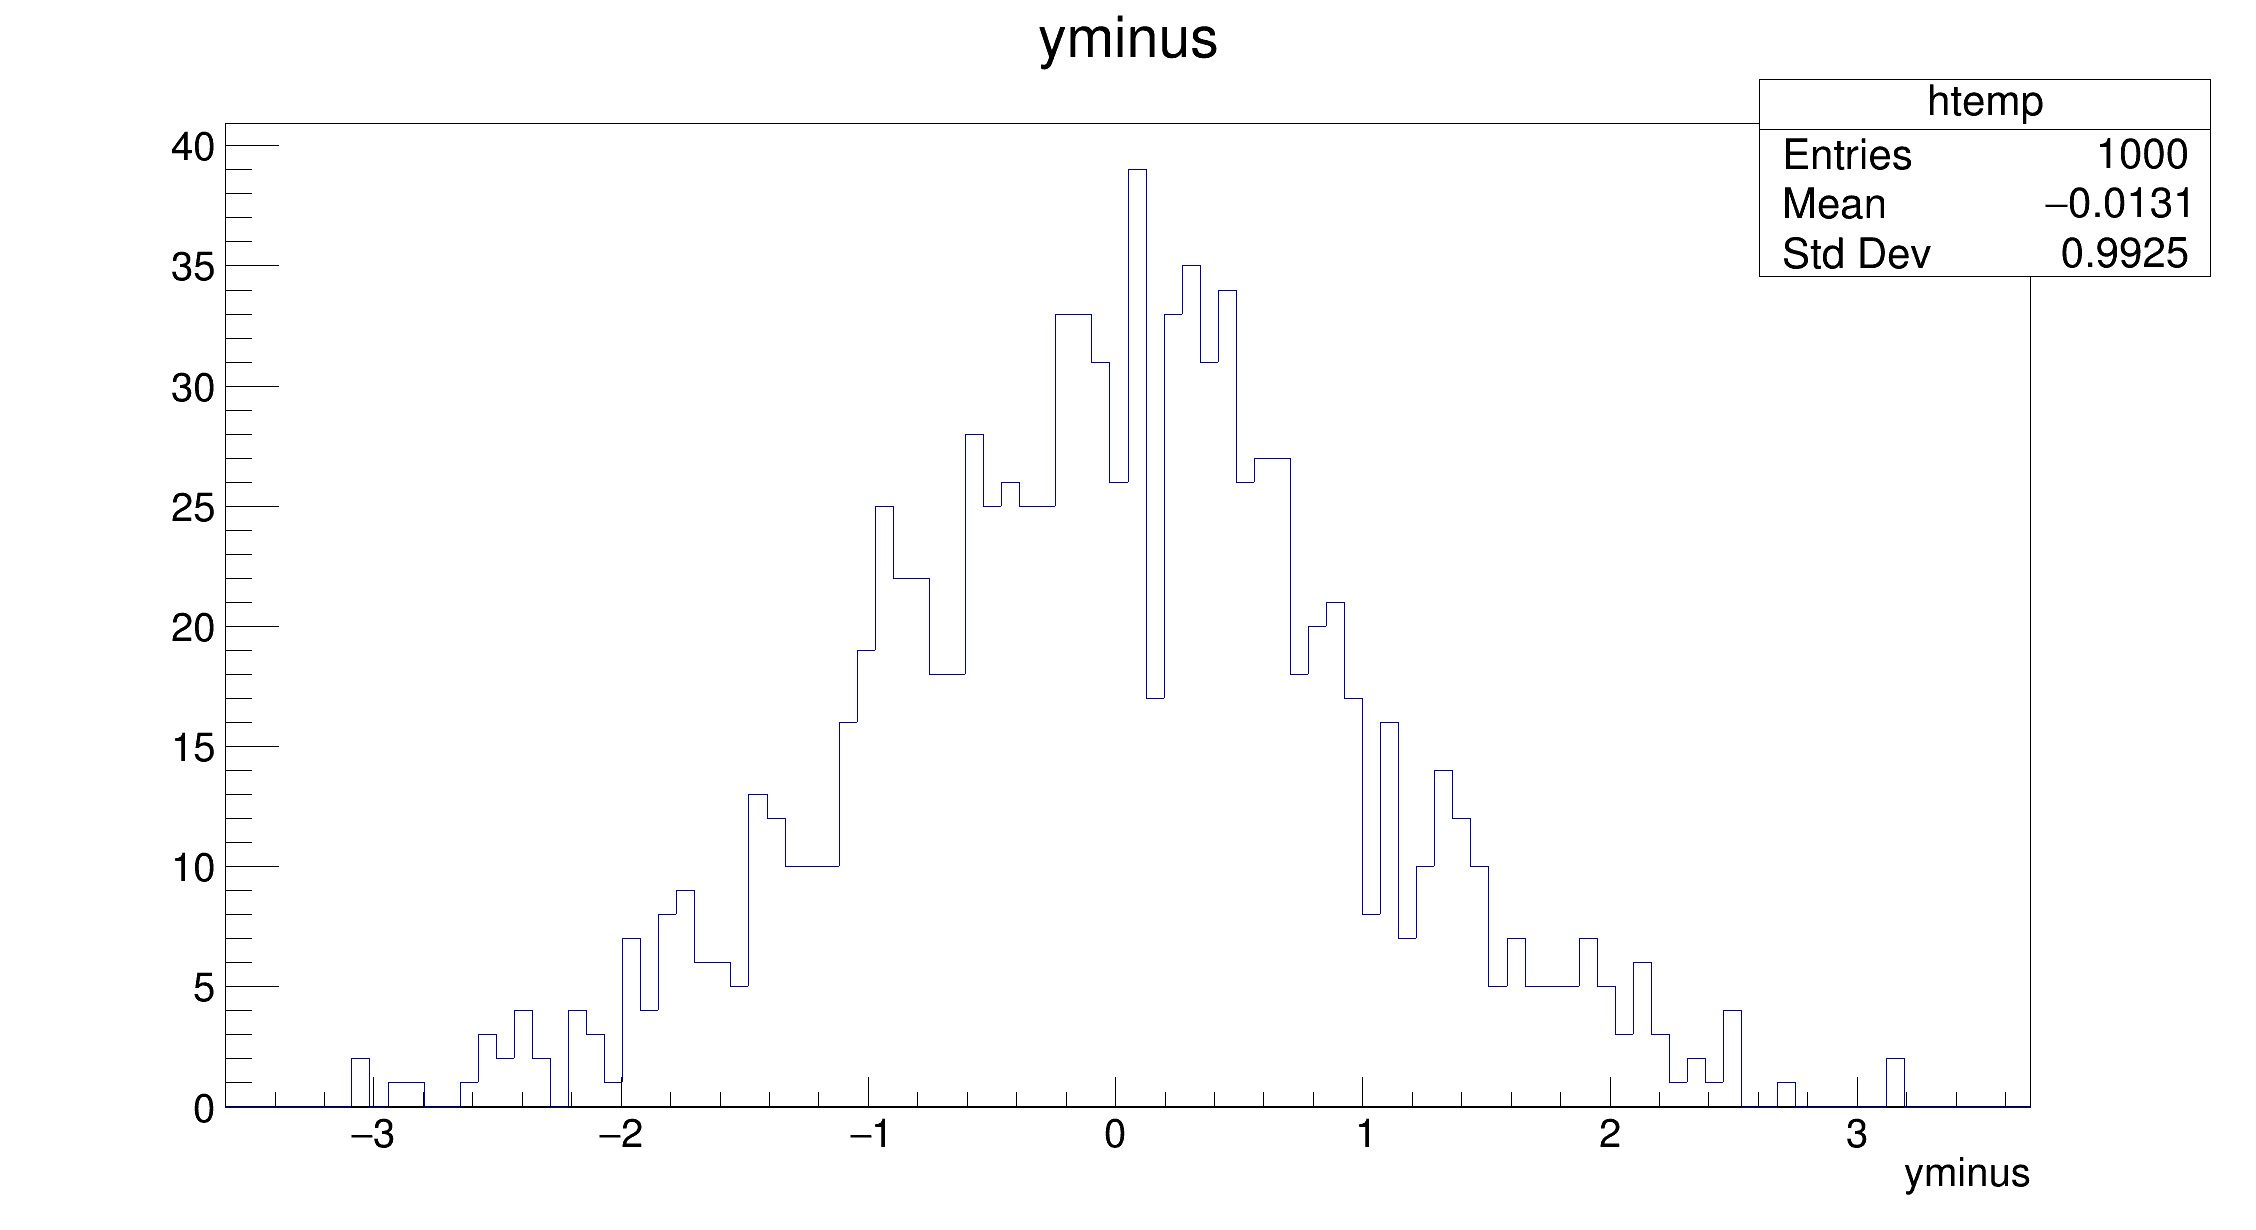
\includegraphics[width = 1.0\textwidth]{NaivePulls/yminus1K1K.png}
      \caption{$y_-$ pull}
    \end{subfigure}
  \end{figure}
\end{frame}

\section{Attempts at better binning scheme}
\subsection{Rectangular binning scheme}
\begin{frame}{Rectangular binning scheme}
  \begin{itemize}
    \item{Inspired by \href{https://arxiv.org/abs/1709.03467}{arXiv:1709.03467}}
    \item{$4$-body phase space is $5$-dimensional}
    \item{Convenient to choose rectangular coordinates}
  \end{itemize}
  \begin{block}{Phase space parameterisation}
    \begin{align*}
      x_1 =& m(K^+\pi^+) + \alpha \\
      x_2 =& m(K^-\pi^-) + \alpha, \quad \alpha = \text{min}\big(m(K^+\pi^+), m(K^-\pi^-)\big) - m_\pi - m_K \\
      x_3 =& \cos(\theta_+), \quad \text{(Helicity angles)} \\
      x_4 =& \cos(\theta_-) \\
      x_5 =& \phi \\
    \end{align*}
  \end{block}
  \begin{itemize}
    \item{Study phase space in terms of these coordinates}
  \end{itemize}
\end{frame}

\begin{frame}{Rectangular binning scheme}
  \begin{figure}
    \centering
    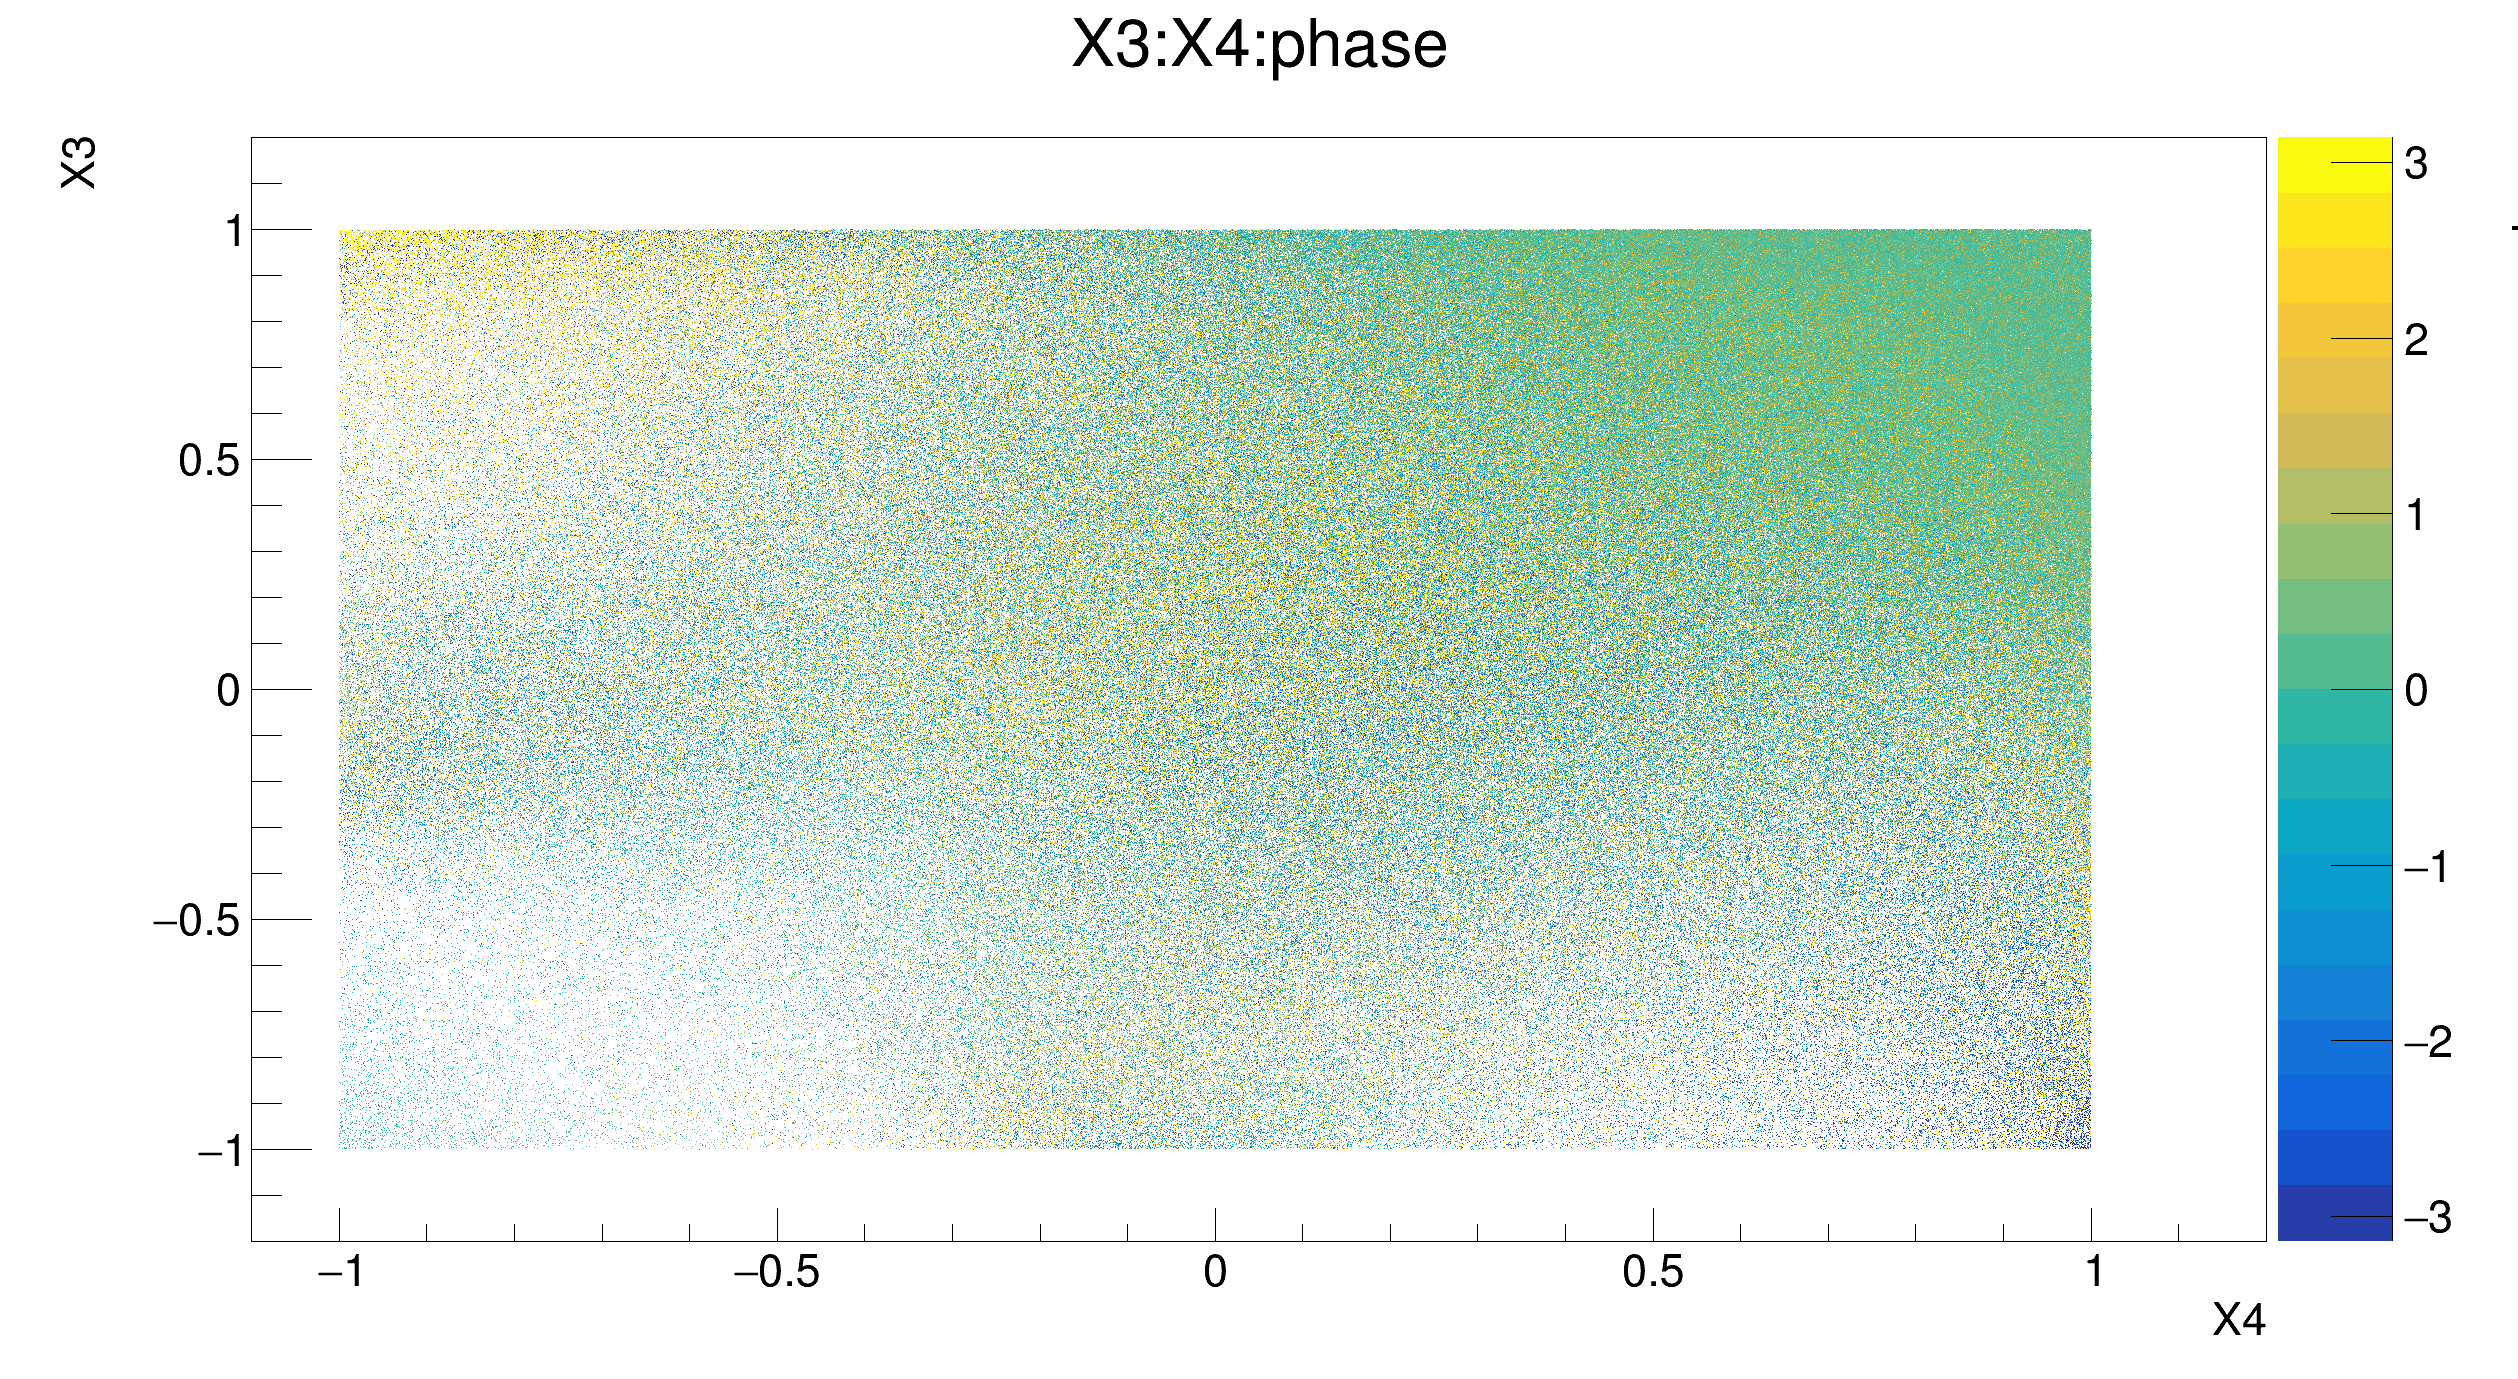
\includegraphics[width = 1.0\textwidth]{X3X4Phase.png}
    \caption{Strong phase differences in the $(x_3, x_4)$ plane}
  \end{figure}
\end{frame}

\begin{frame}{Rectangular binning scheme}
  \begin{figure}
    \centering
    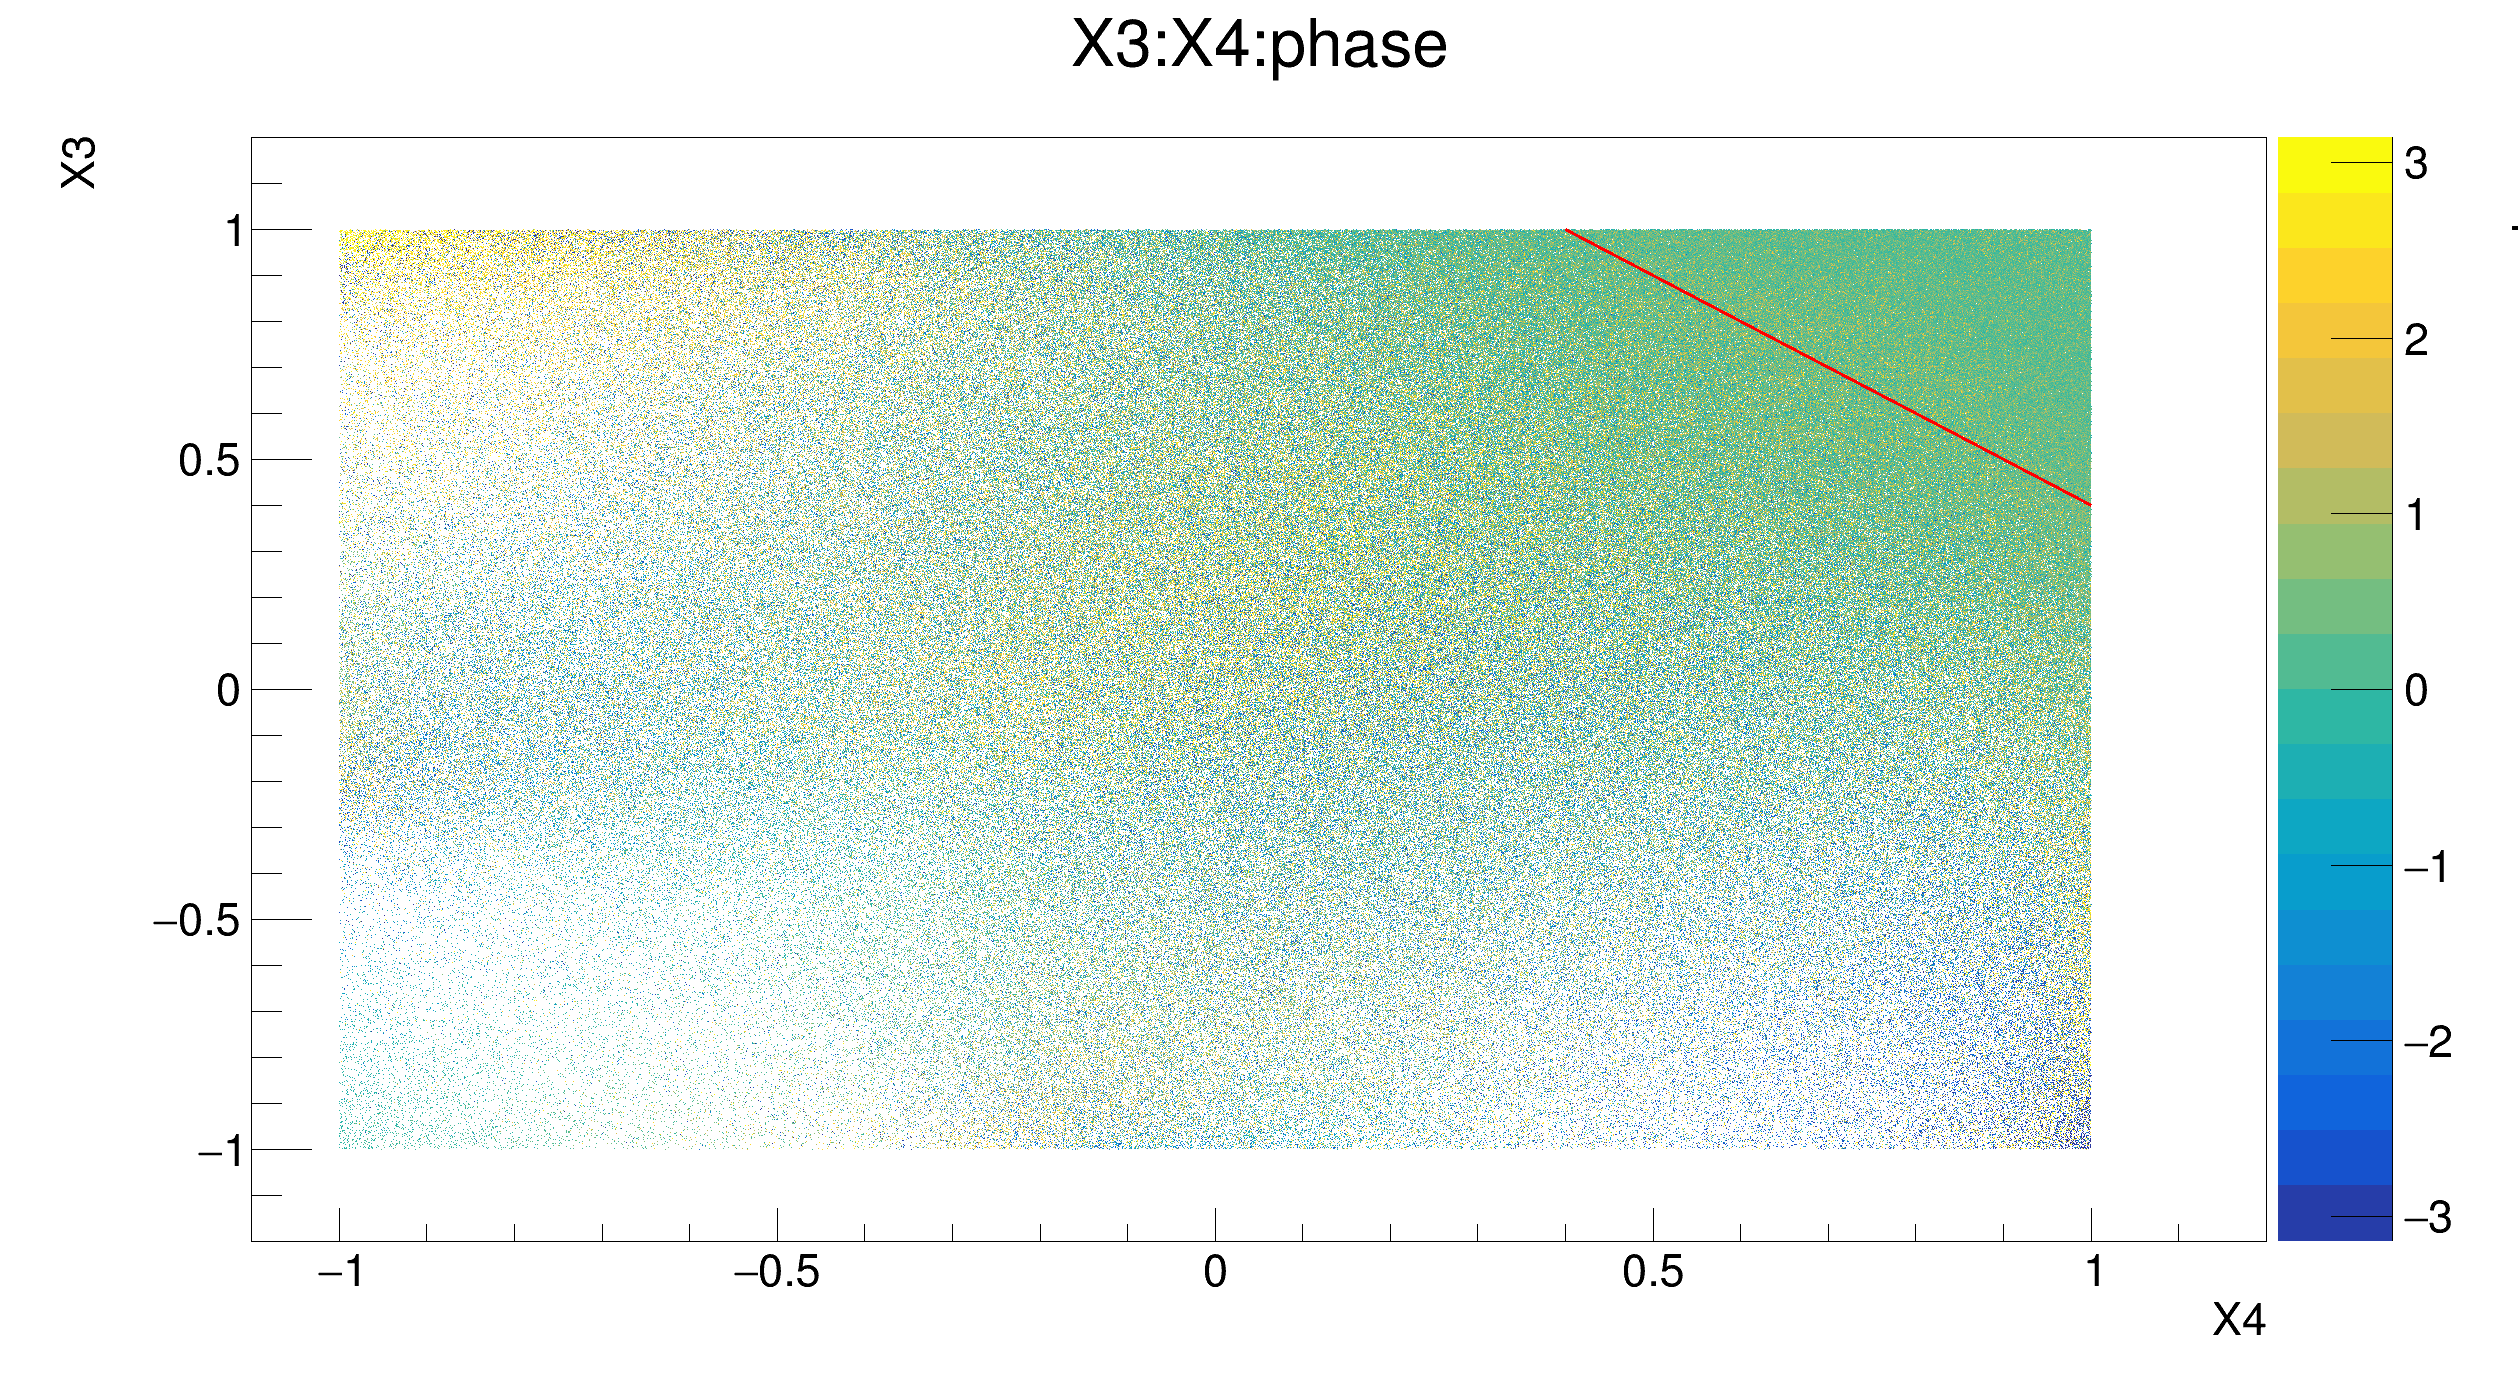
\includegraphics[width = 1.0\textwidth]{X3X4PhaseRegion1.png}
    \caption{Strong phase differences in the $(x_3, x_4)$ plane}
  \end{figure}
\end{frame}

\begin{frame}{Rectangular binning scheme}
  \begin{figure}
    \centering
    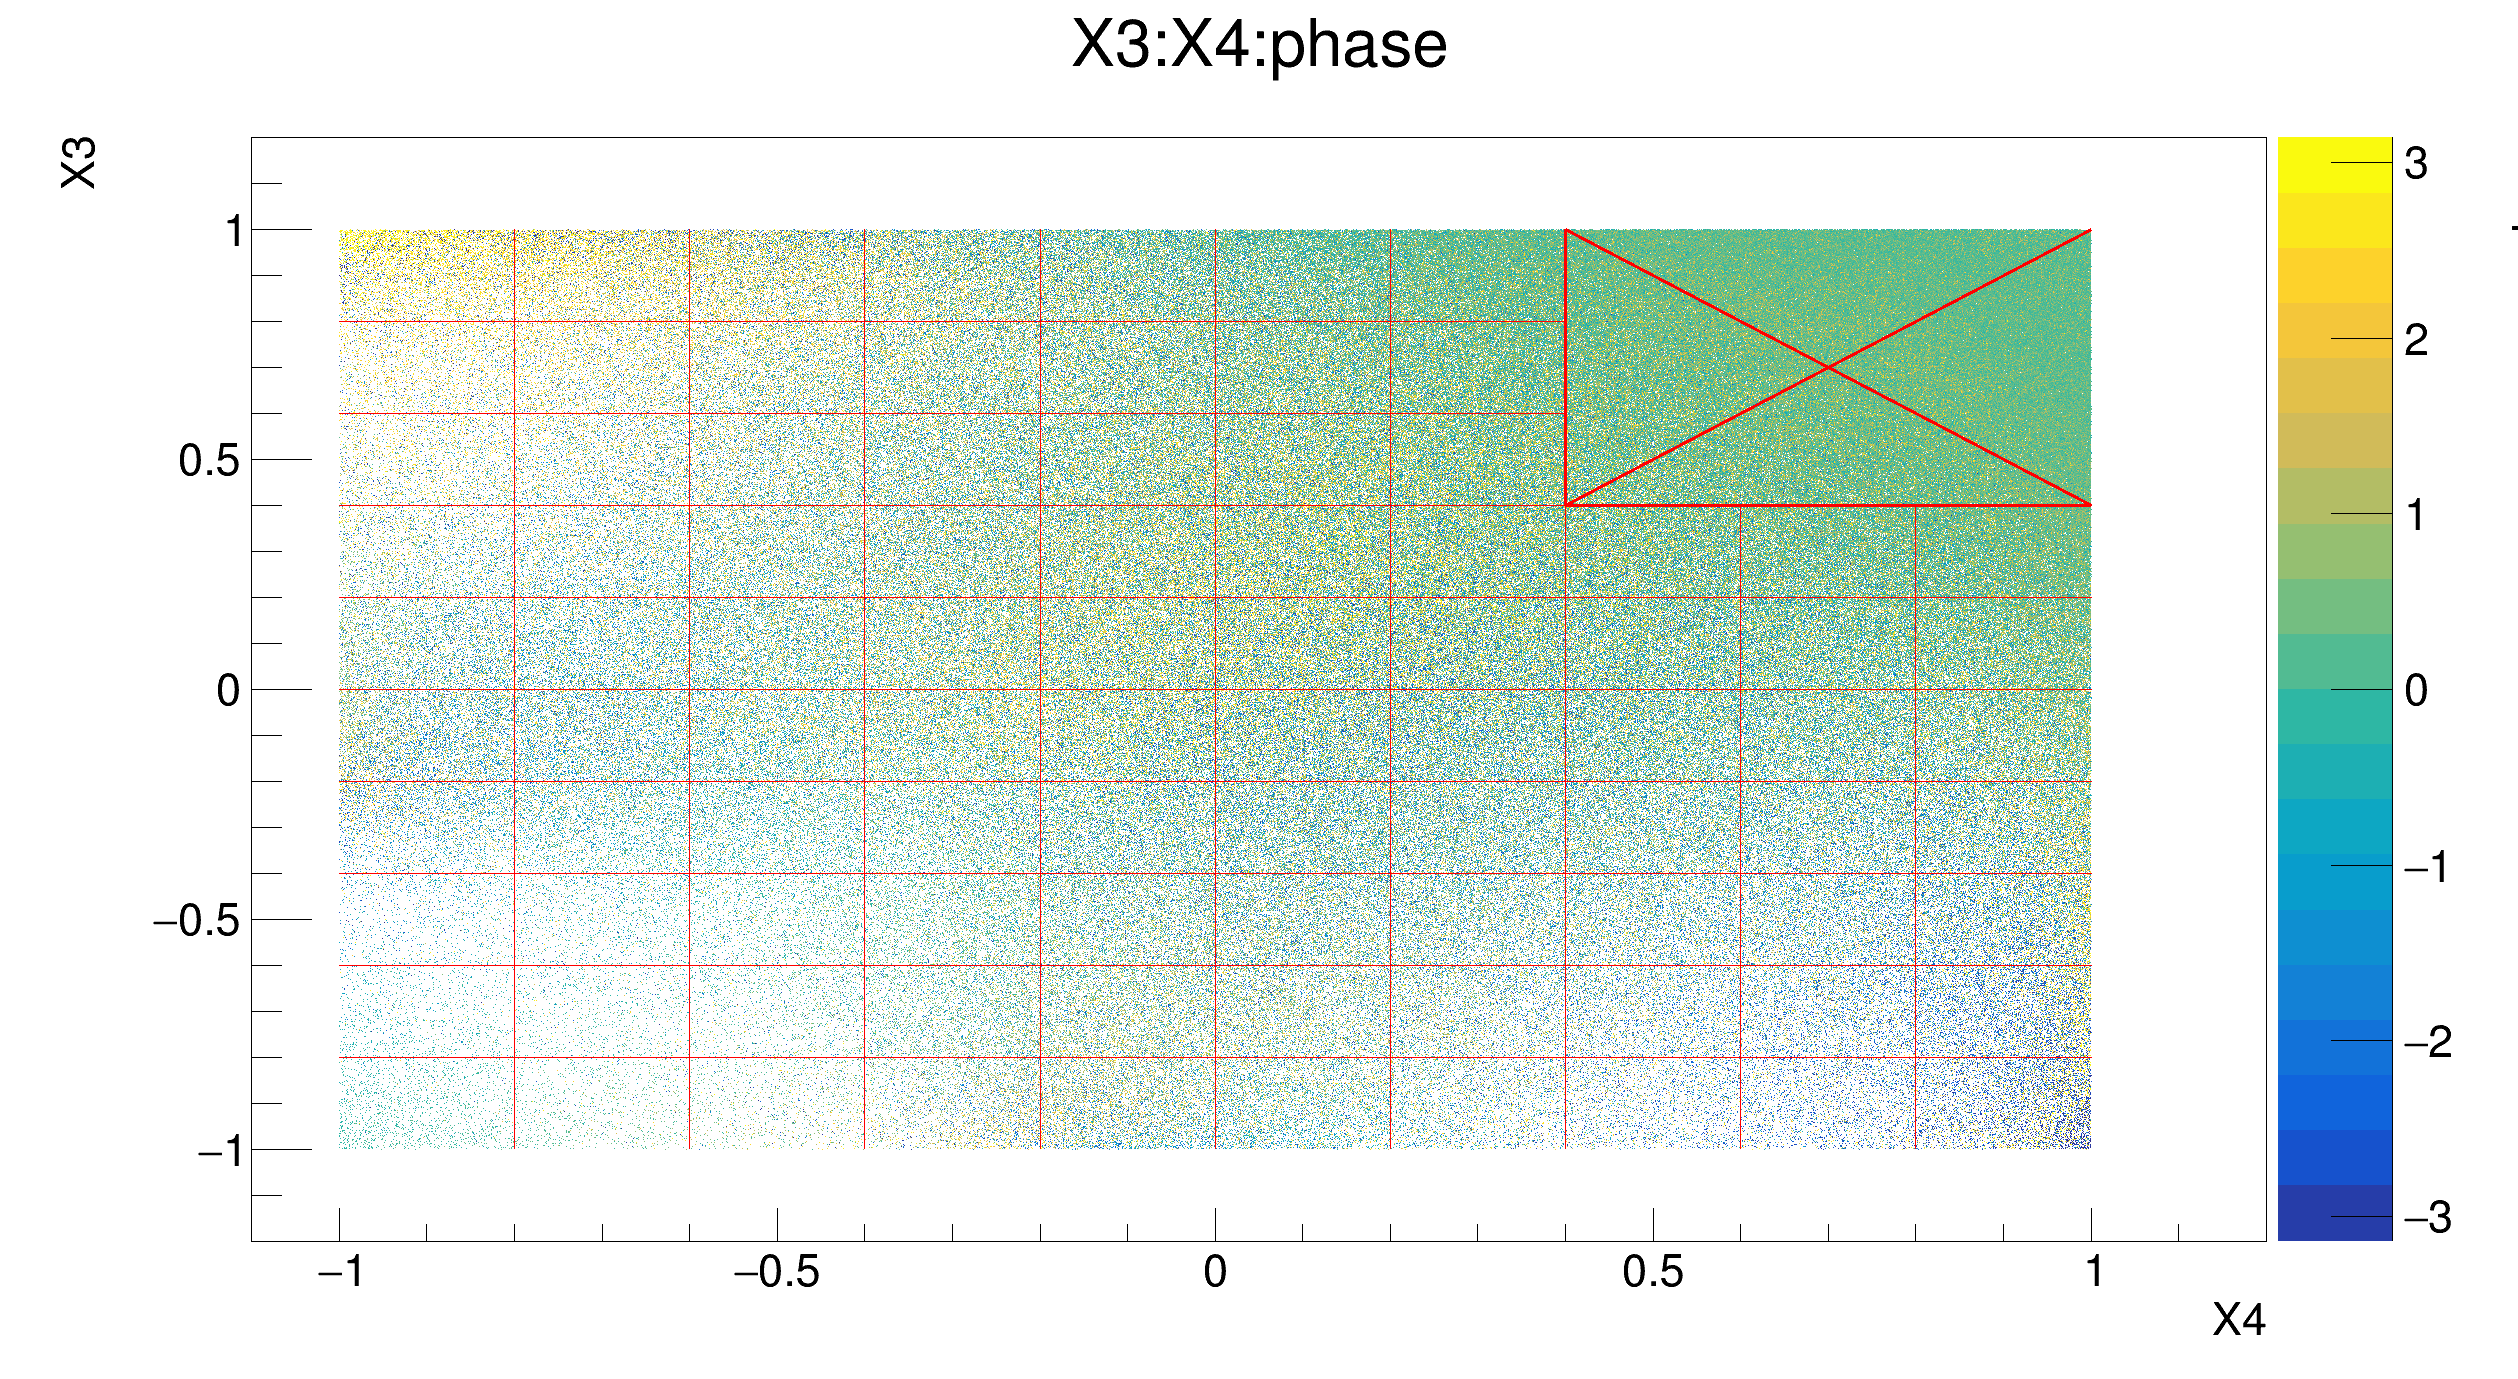
\includegraphics[width = 1.0\textwidth]{X3X4PhaseRegions.png}
    \caption{Strong phase differences in the $(x_3, x_4)$ plane}
  \end{figure}
\end{frame}

\begin{frame}{Description of rectangular scheme}
  \begin{itemize}
    \item{Define upper right corner as bin $0$ and $1$}
    \item{Divide the $(x_3, x_4)$ plane into regions}
    \item{Make a $100\times 100\times 100$ grid in $(x_1, x_2, x_5)$ volume}
    \item{For each gridpoint in $(x_1, x_2, x_5)$, average strong phases over $(x_3, x_4)$}
    \item{Sort each gridpoint into one of $6$ bins according to strong phase}
    \item{$6 + 2 = 8$ bins}
  \end{itemize}
\end{frame}

\begin{frame}{Pull study with $\SI{2e3}{}$ events}
  \begin{figure}
    \centering
    \vspace{-0.2cm}
    \begin{subfigure}{0.5\textwidth}
      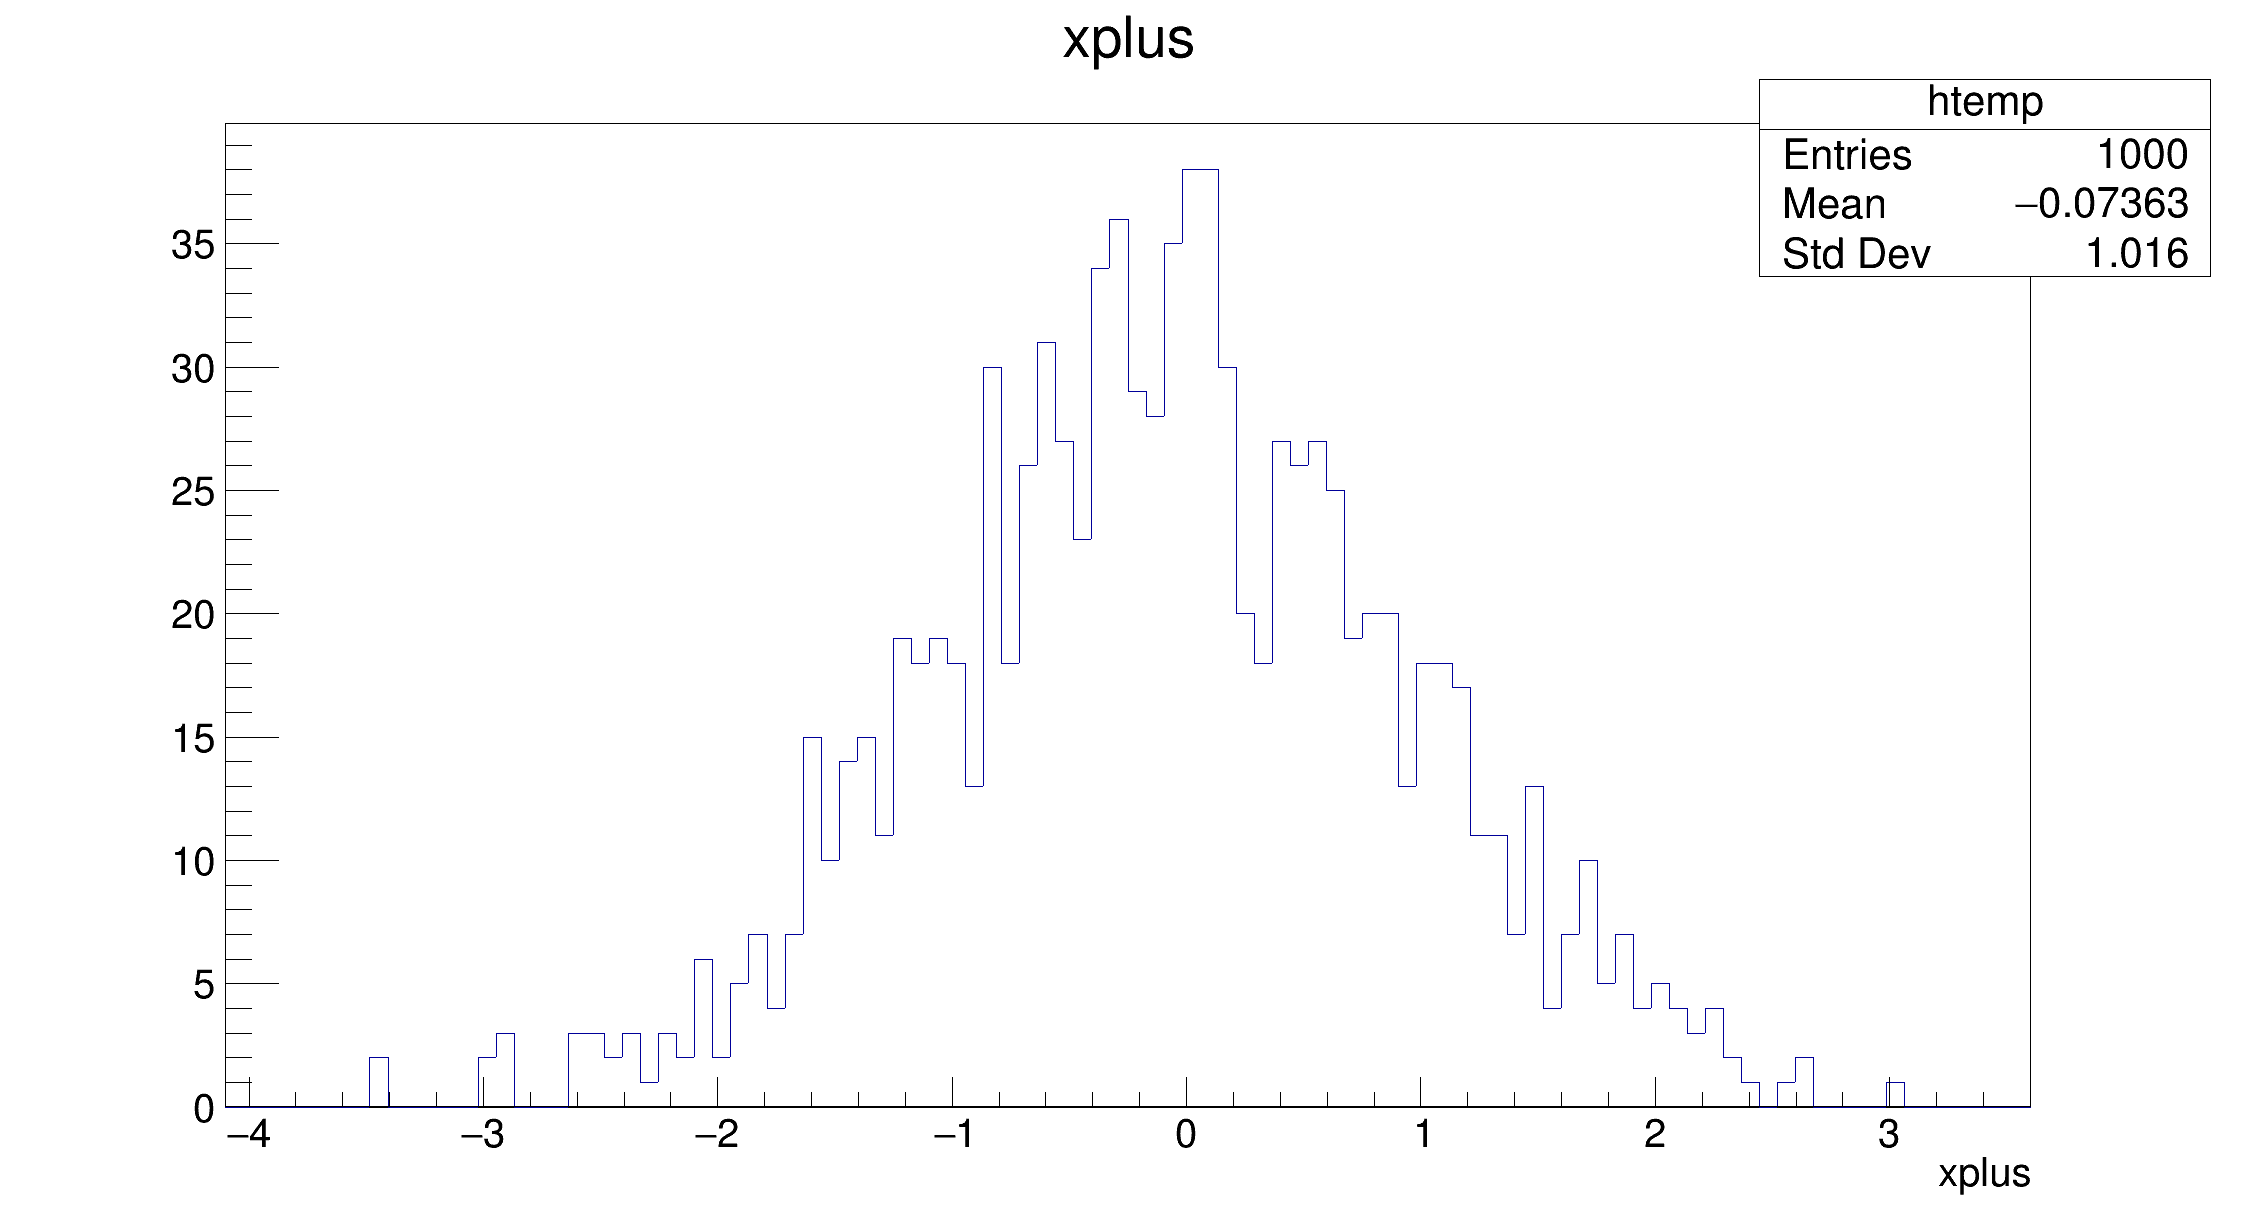
\includegraphics[width = 1.0\textwidth]{SophisticatedPulls/xplus1K1K.png}
      \caption{$x_+$ pull}
    \end{subfigure}%
    \begin{subfigure}{0.5\textwidth}
      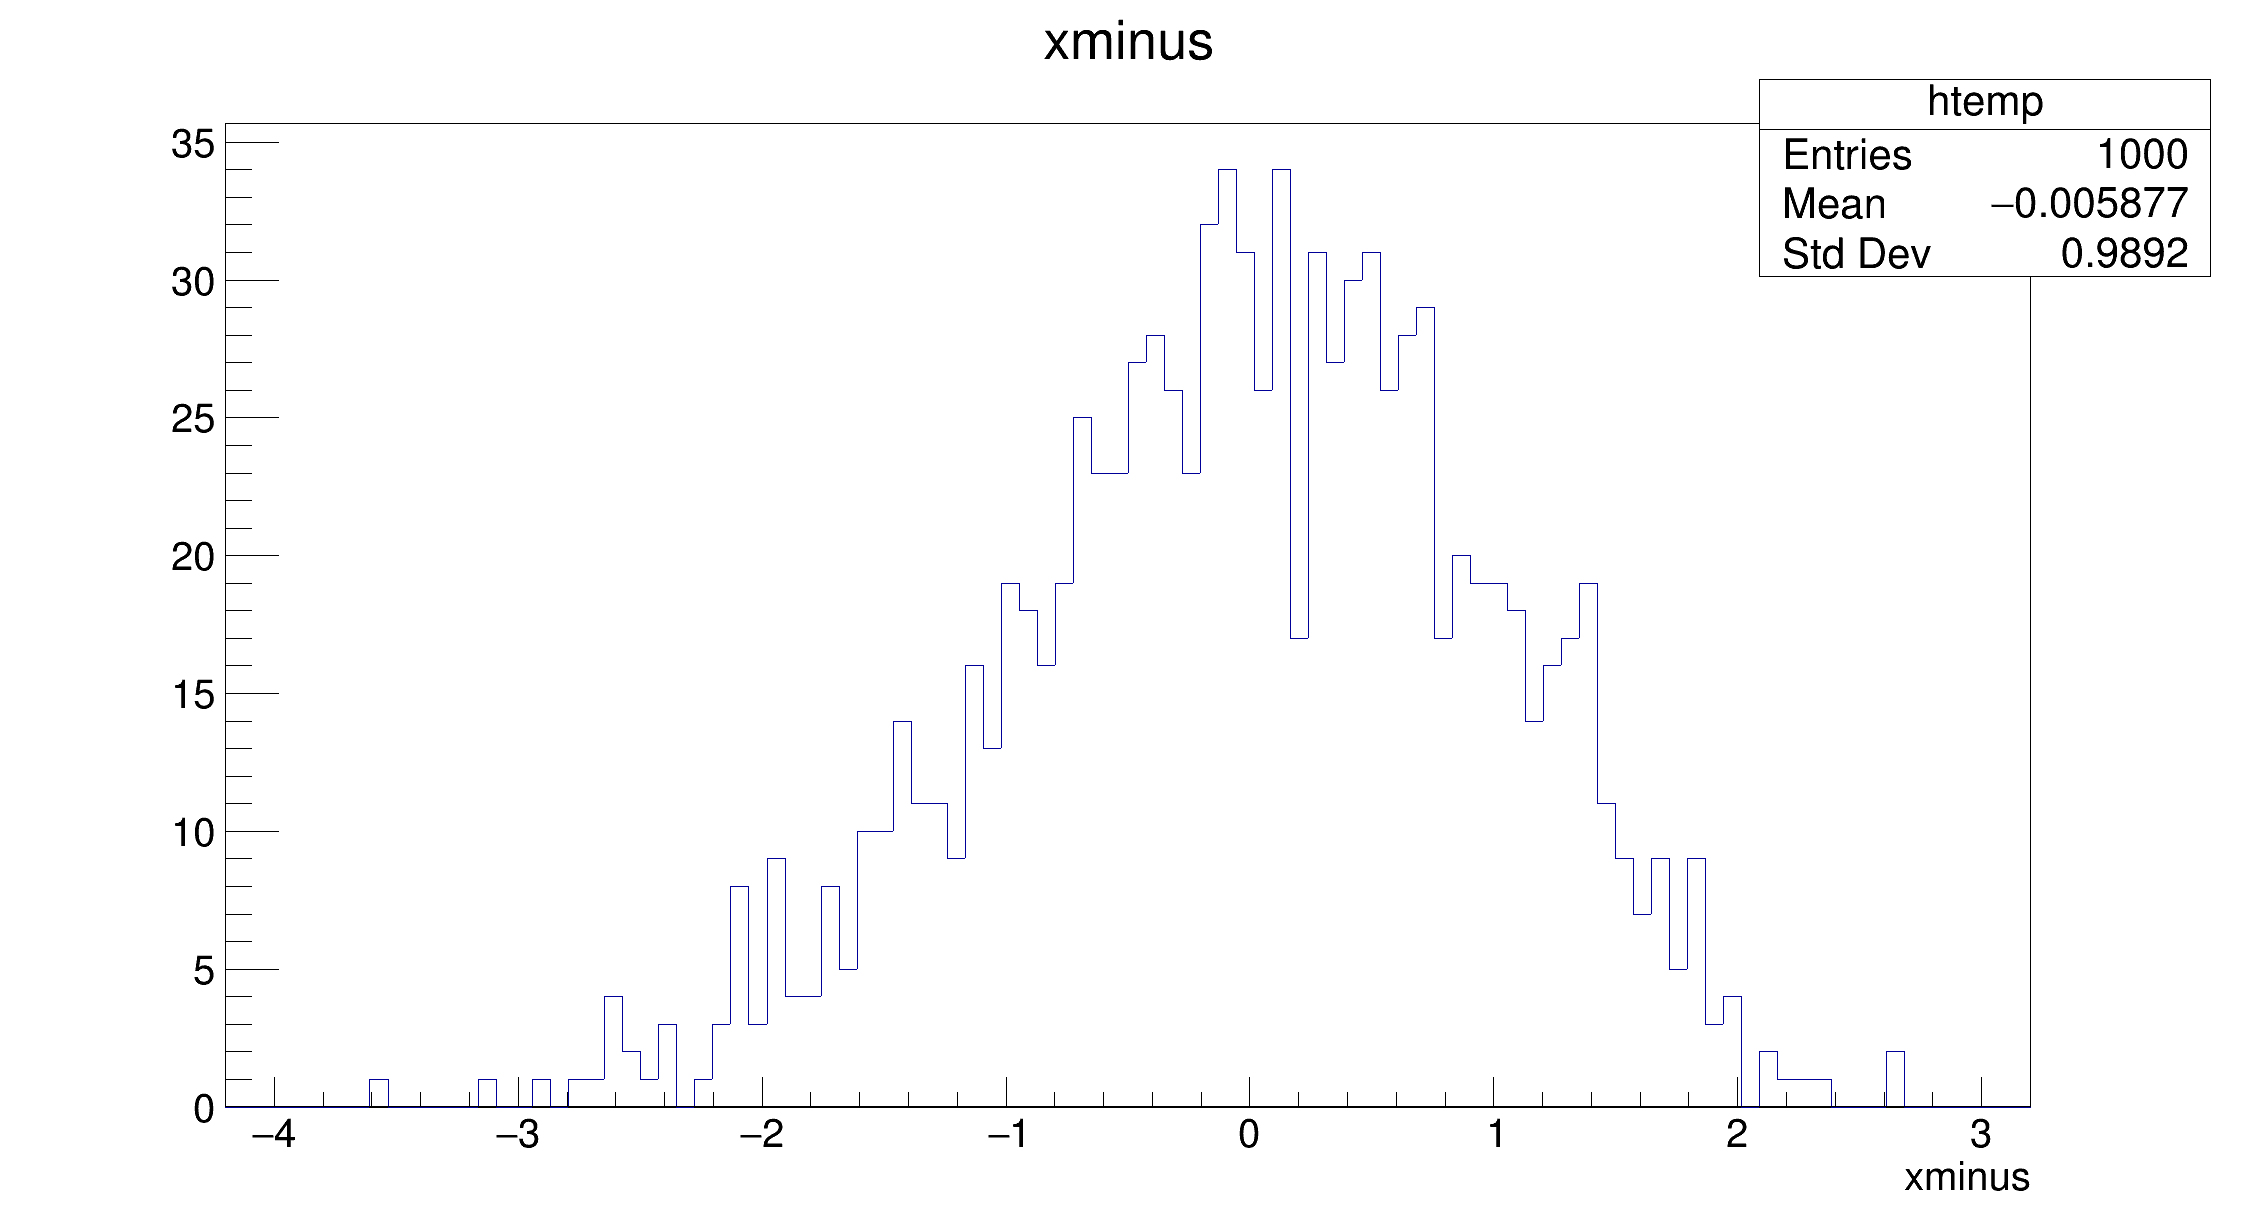
\includegraphics[width = 1.0\textwidth]{SophisticatedPulls/xminus1K1K.png}
      \caption{$x_-$ pull}
    \end{subfigure}
    \begin{subfigure}{0.5\textwidth}
      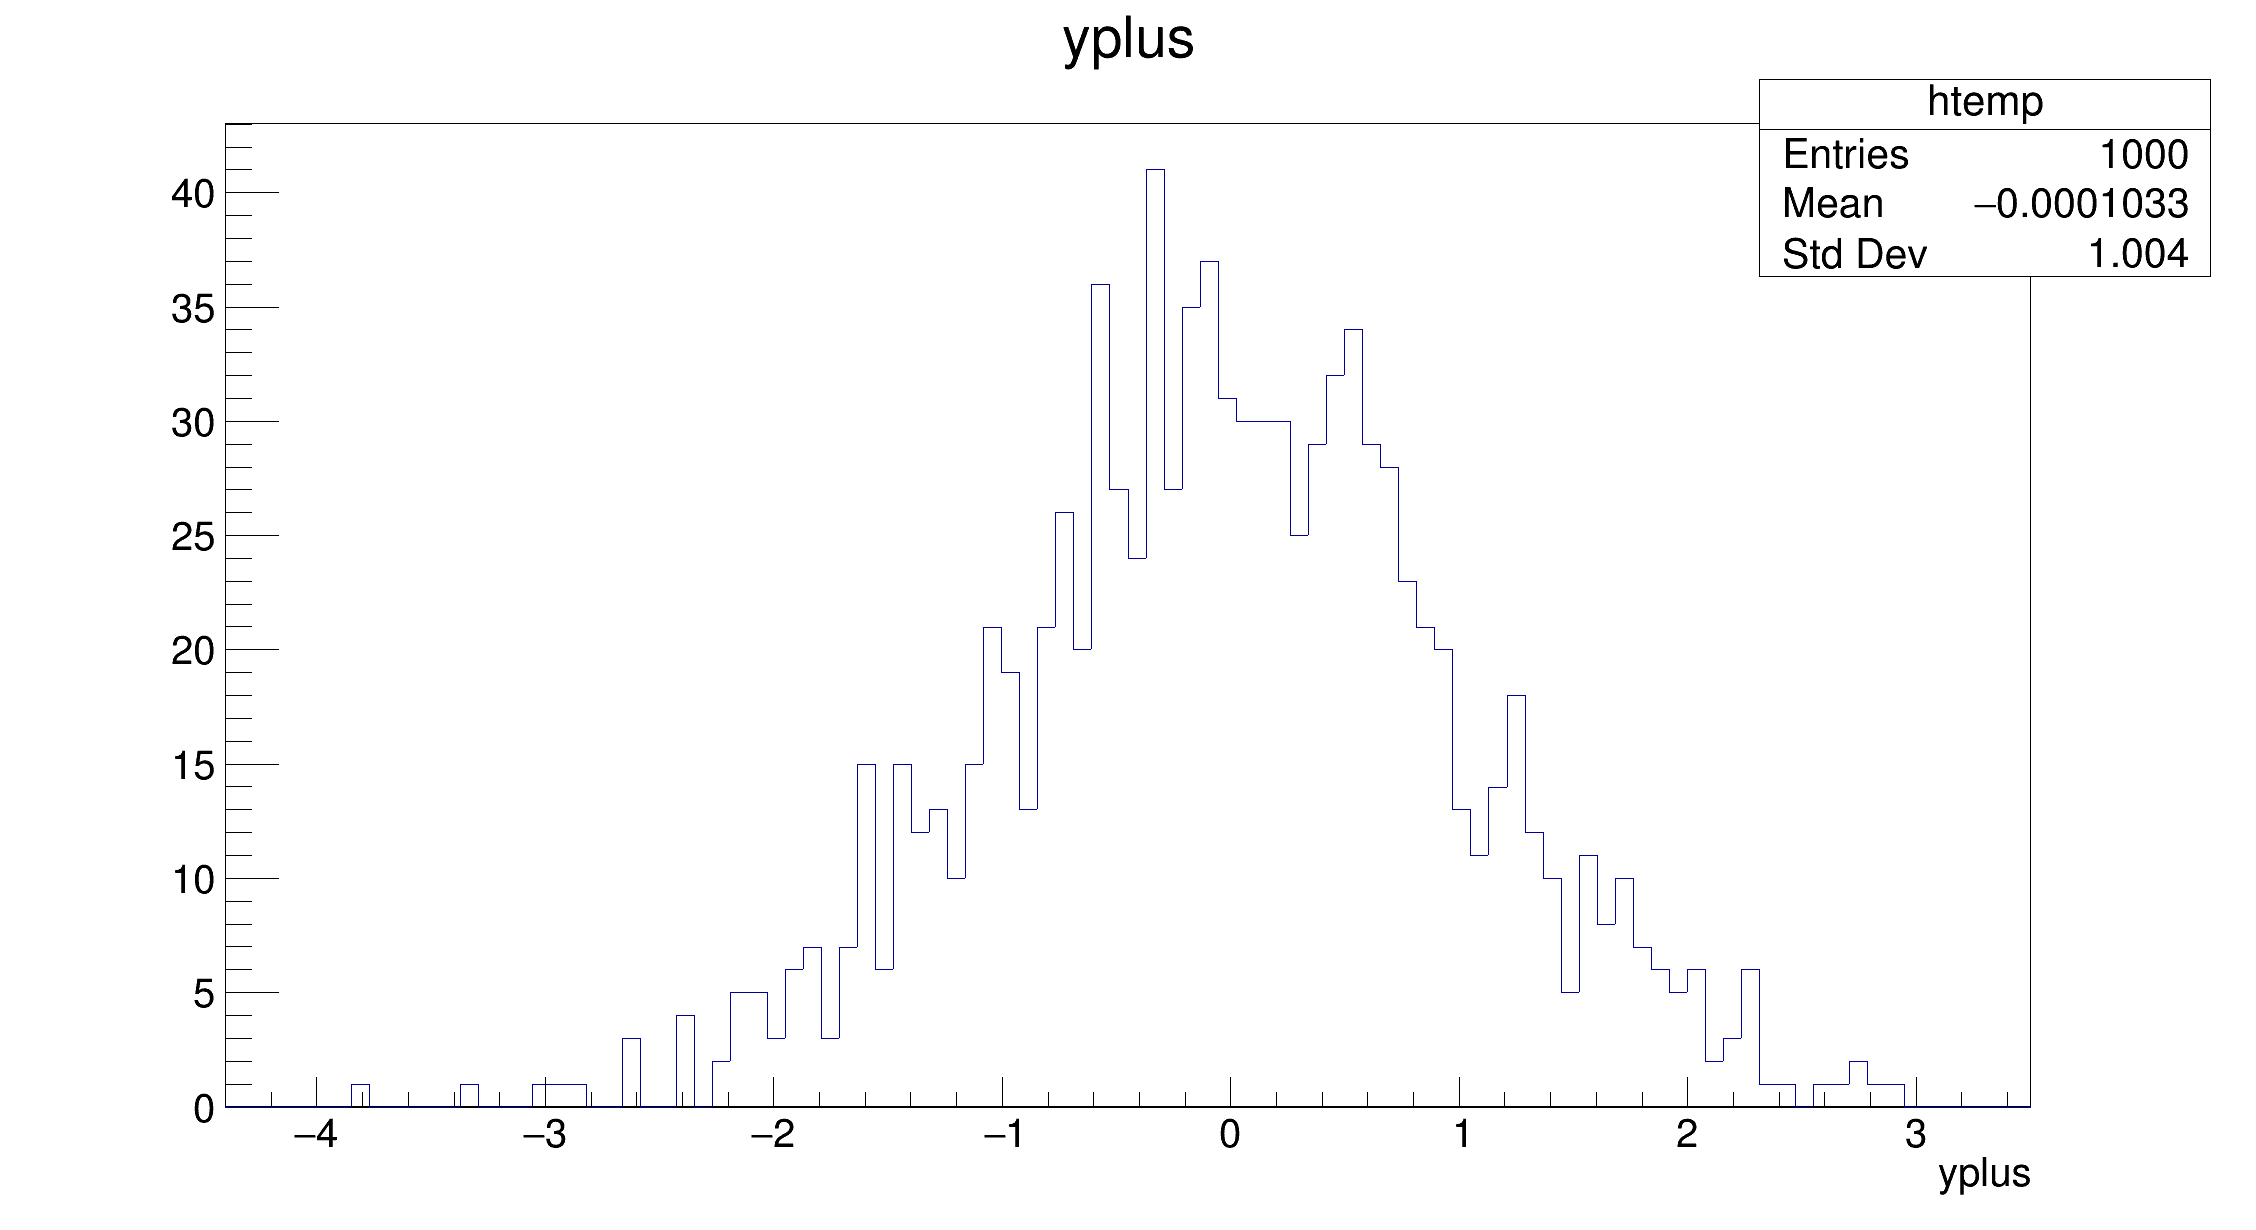
\includegraphics[width = 1.0\textwidth]{SophisticatedPulls/yplus1K1K.png}
      \caption{$y_+$ pull}
    \end{subfigure}%
    \begin{subfigure}{0.5\textwidth}
      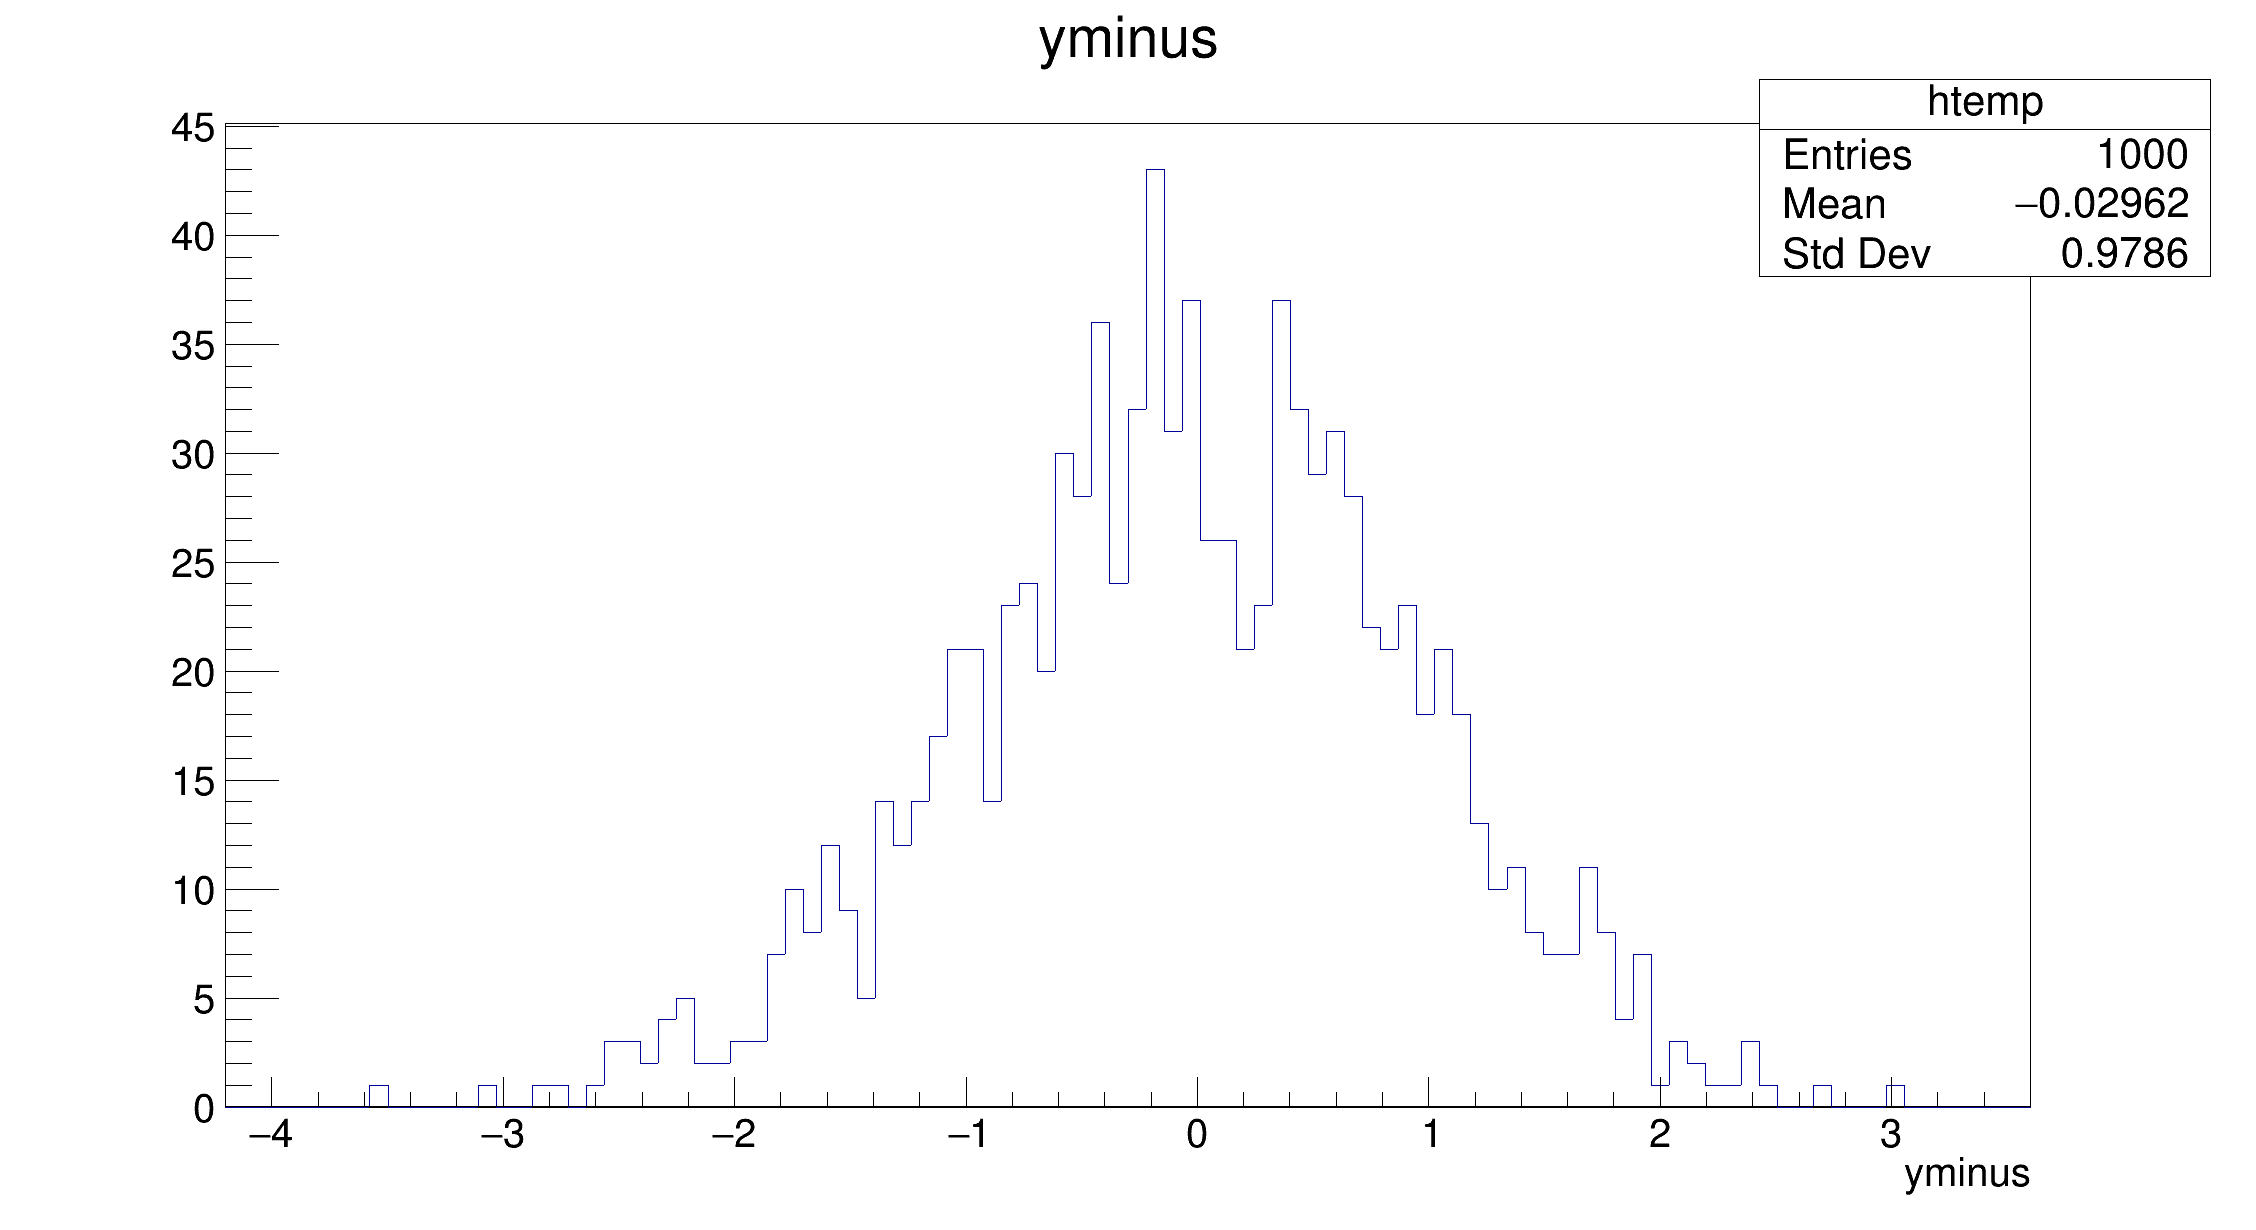
\includegraphics[width = 1.0\textwidth]{SophisticatedPulls/yminus1K1K.png}
      \caption{$y_-$ pull}
    \end{subfigure}
  \end{figure}
\end{frame}

\begin{frame}{Pull study with $\SI{2e3}{}$ events}
  \begin{figure}
    \centering
    \vspace{-0.2cm}
    \begin{subfigure}{0.5\textwidth}
      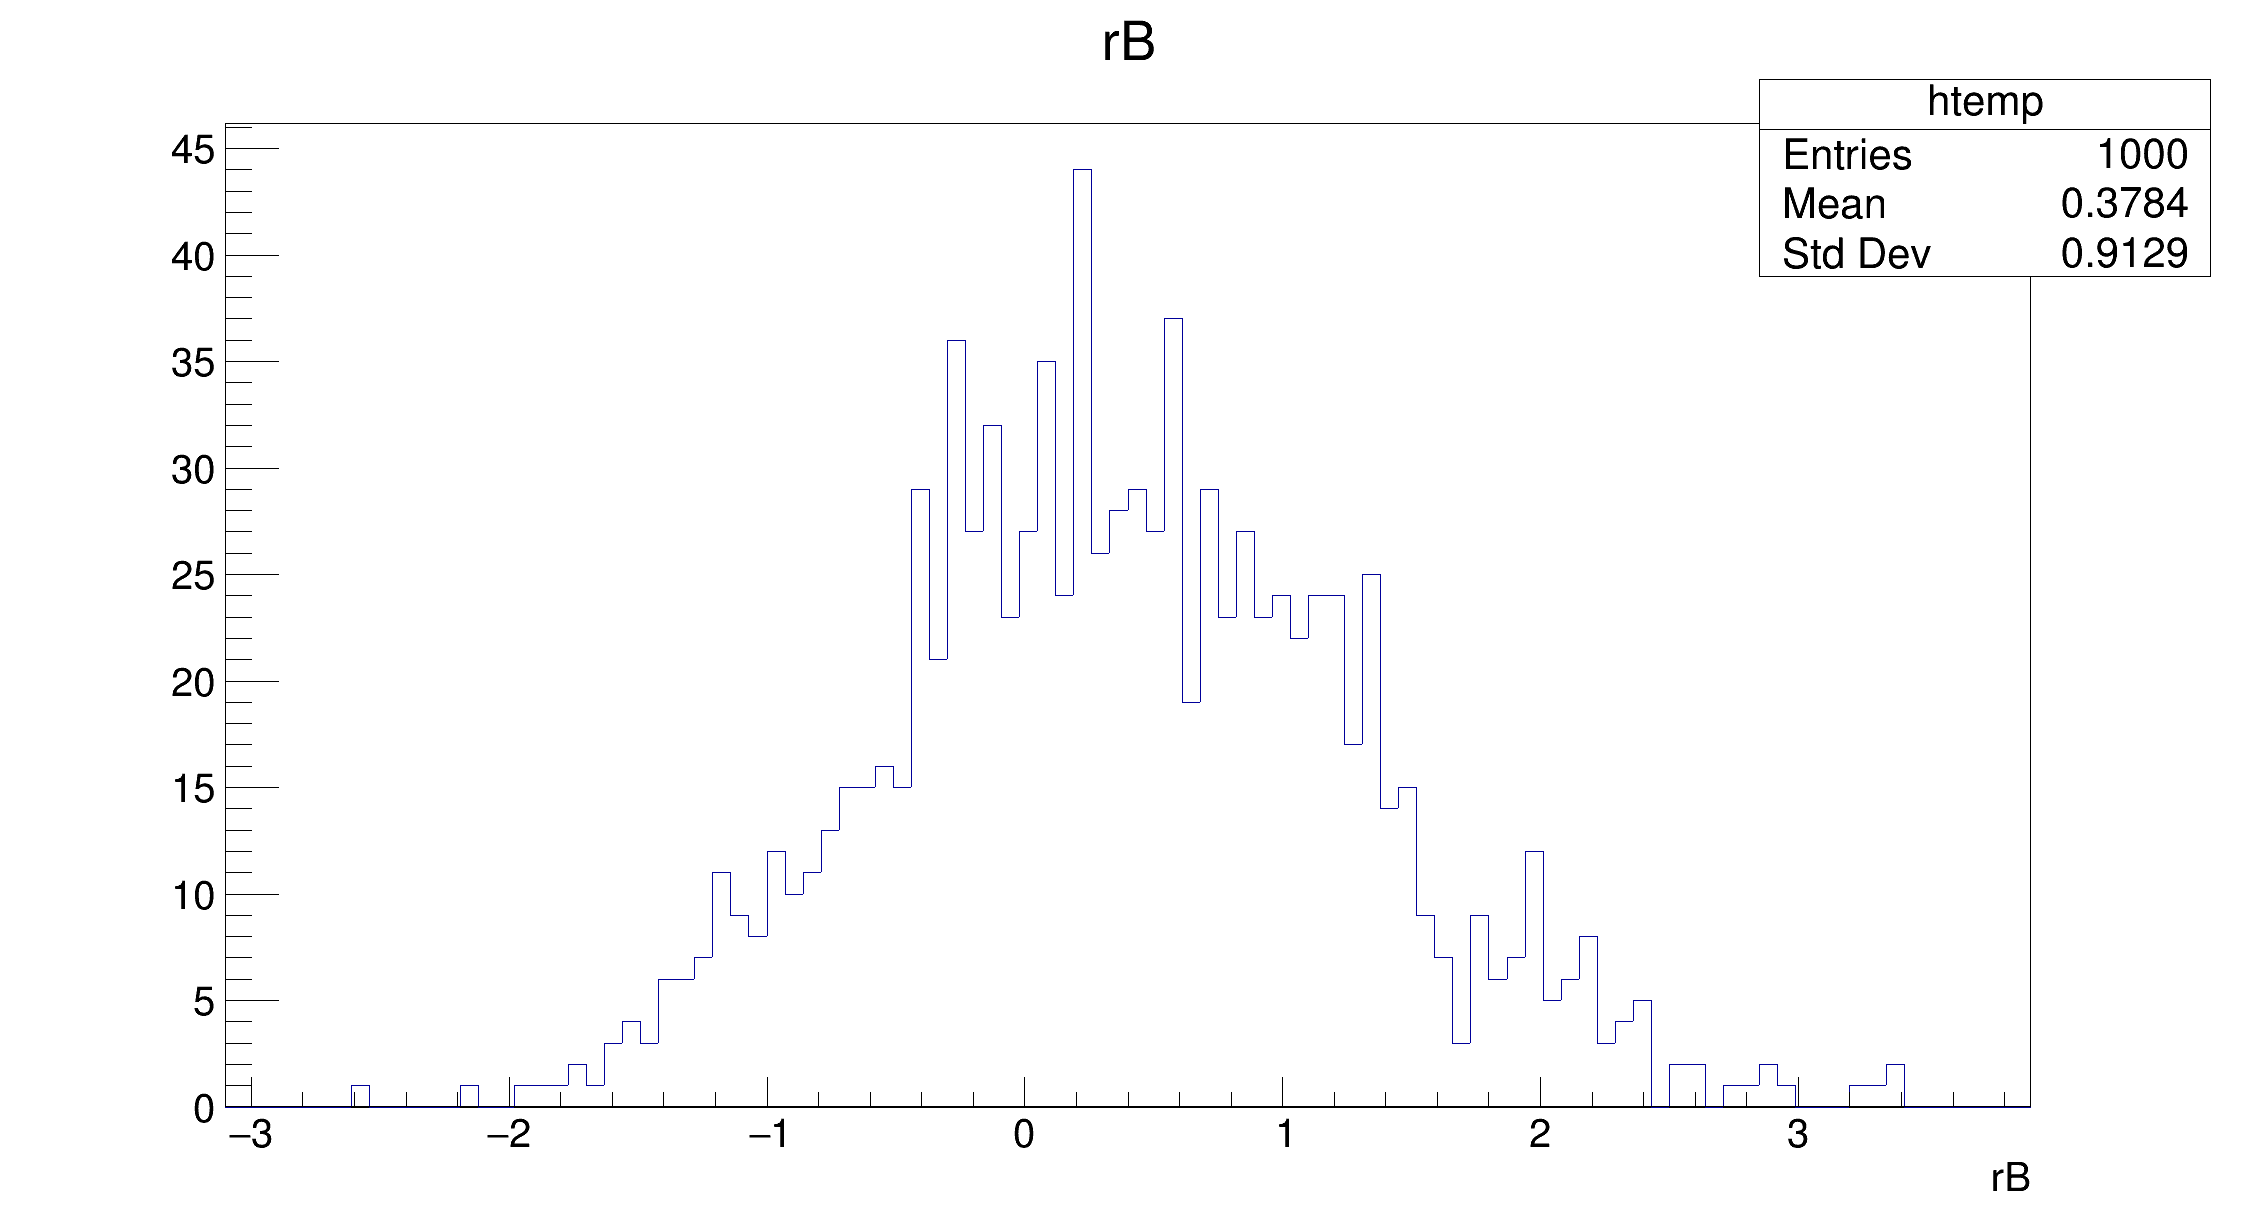
\includegraphics[width = 1.0\textwidth]{SophisticatedPulls/rB1K1K.png}
      \caption{$r_B$ pull}
    \end{subfigure}%
    \begin{subfigure}{0.5\textwidth}
      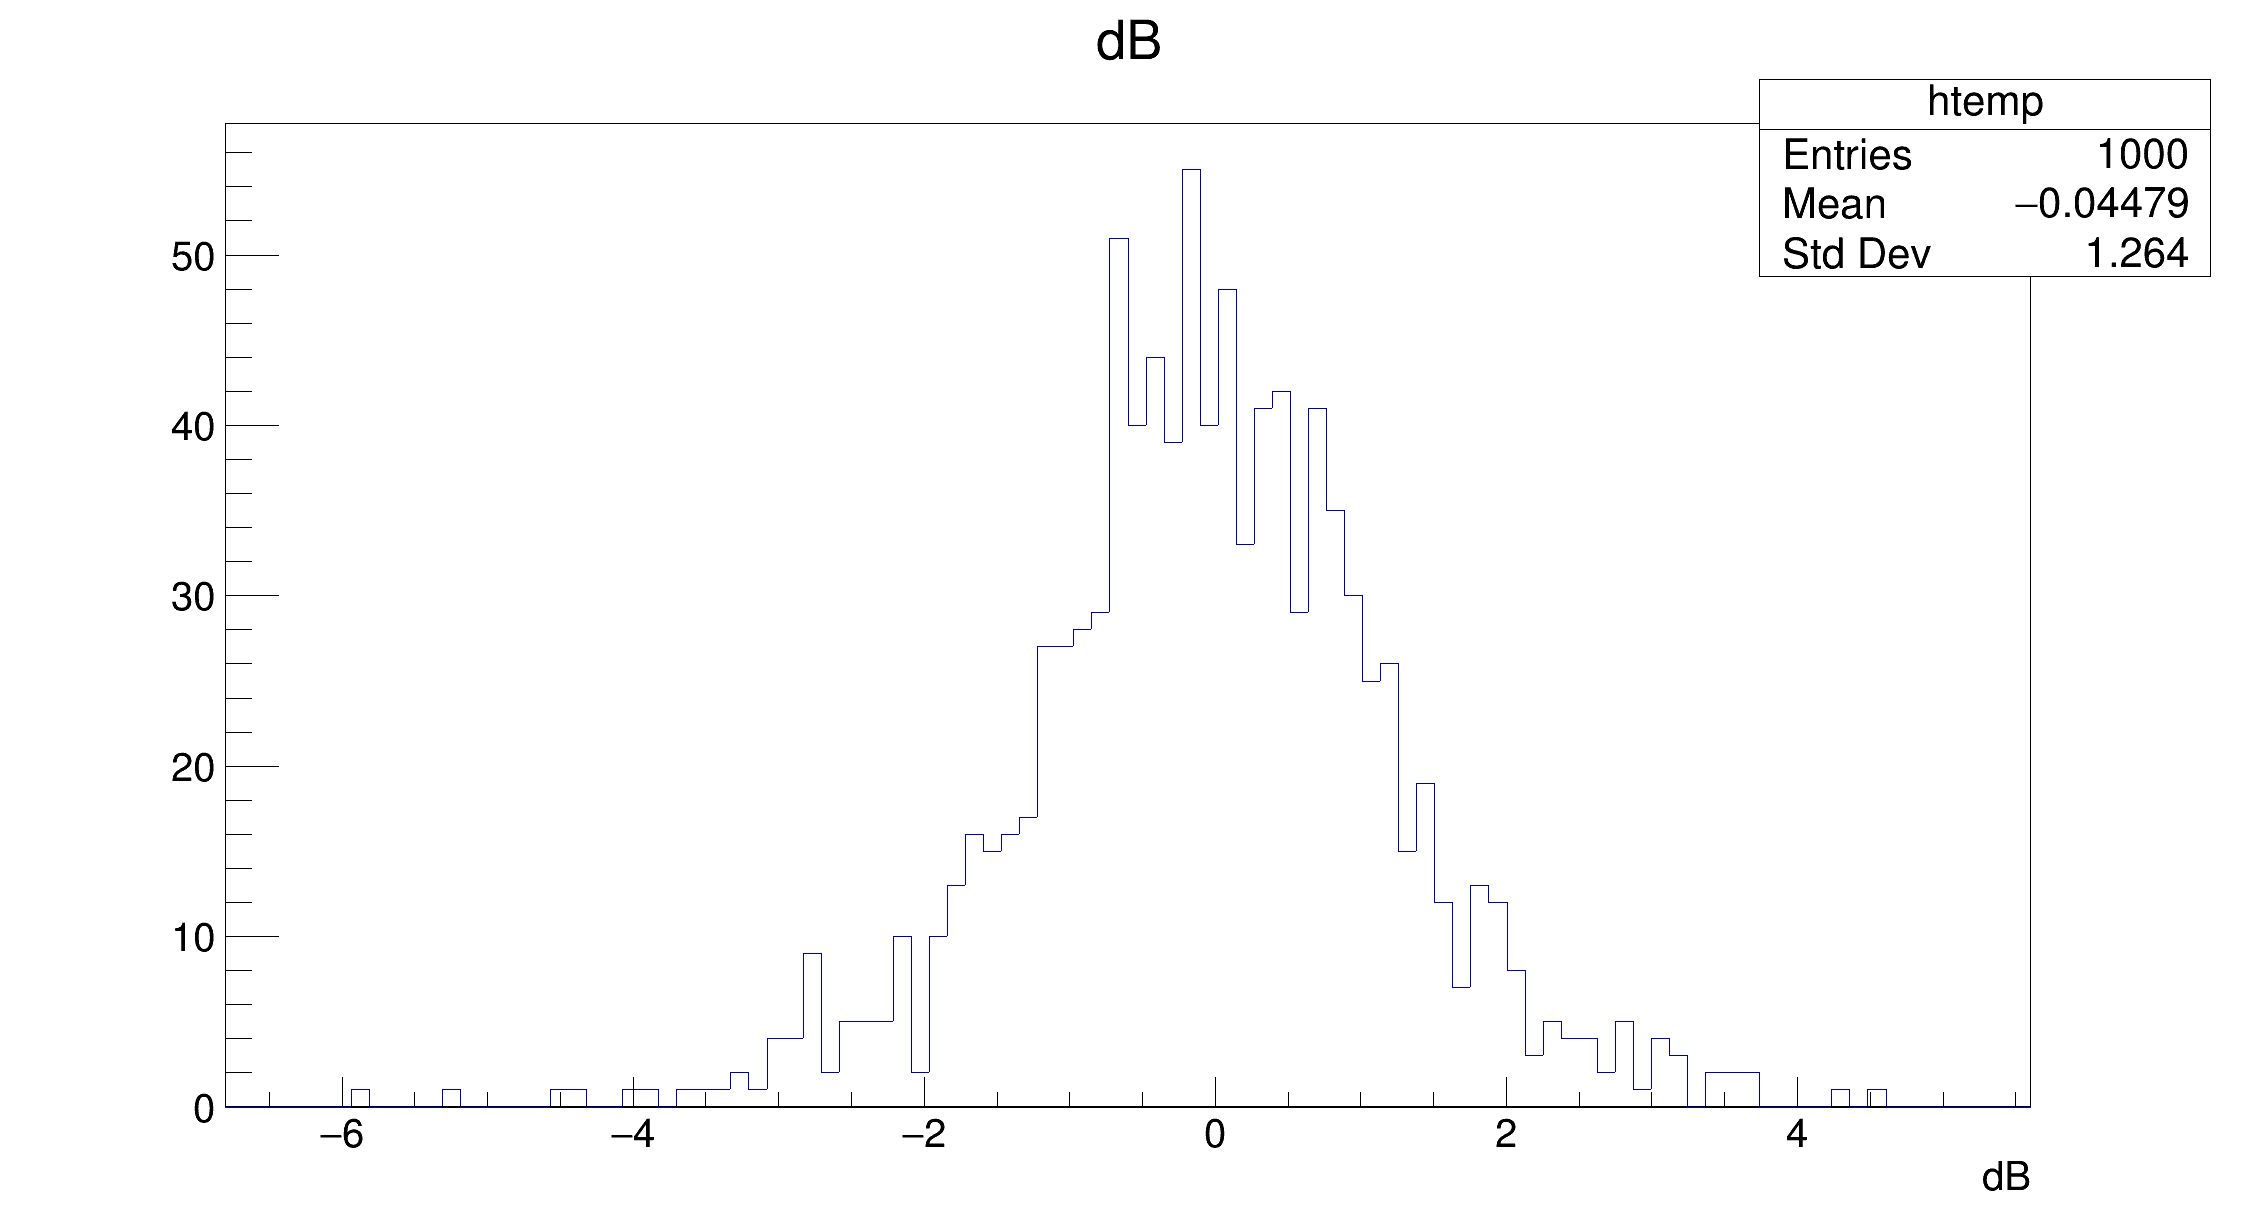
\includegraphics[width = 1.0\textwidth]{SophisticatedPulls/dB1K1K.png}
      \caption{$\delta_B$ pull}
    \end{subfigure}
    \begin{subfigure}{0.5\textwidth}
      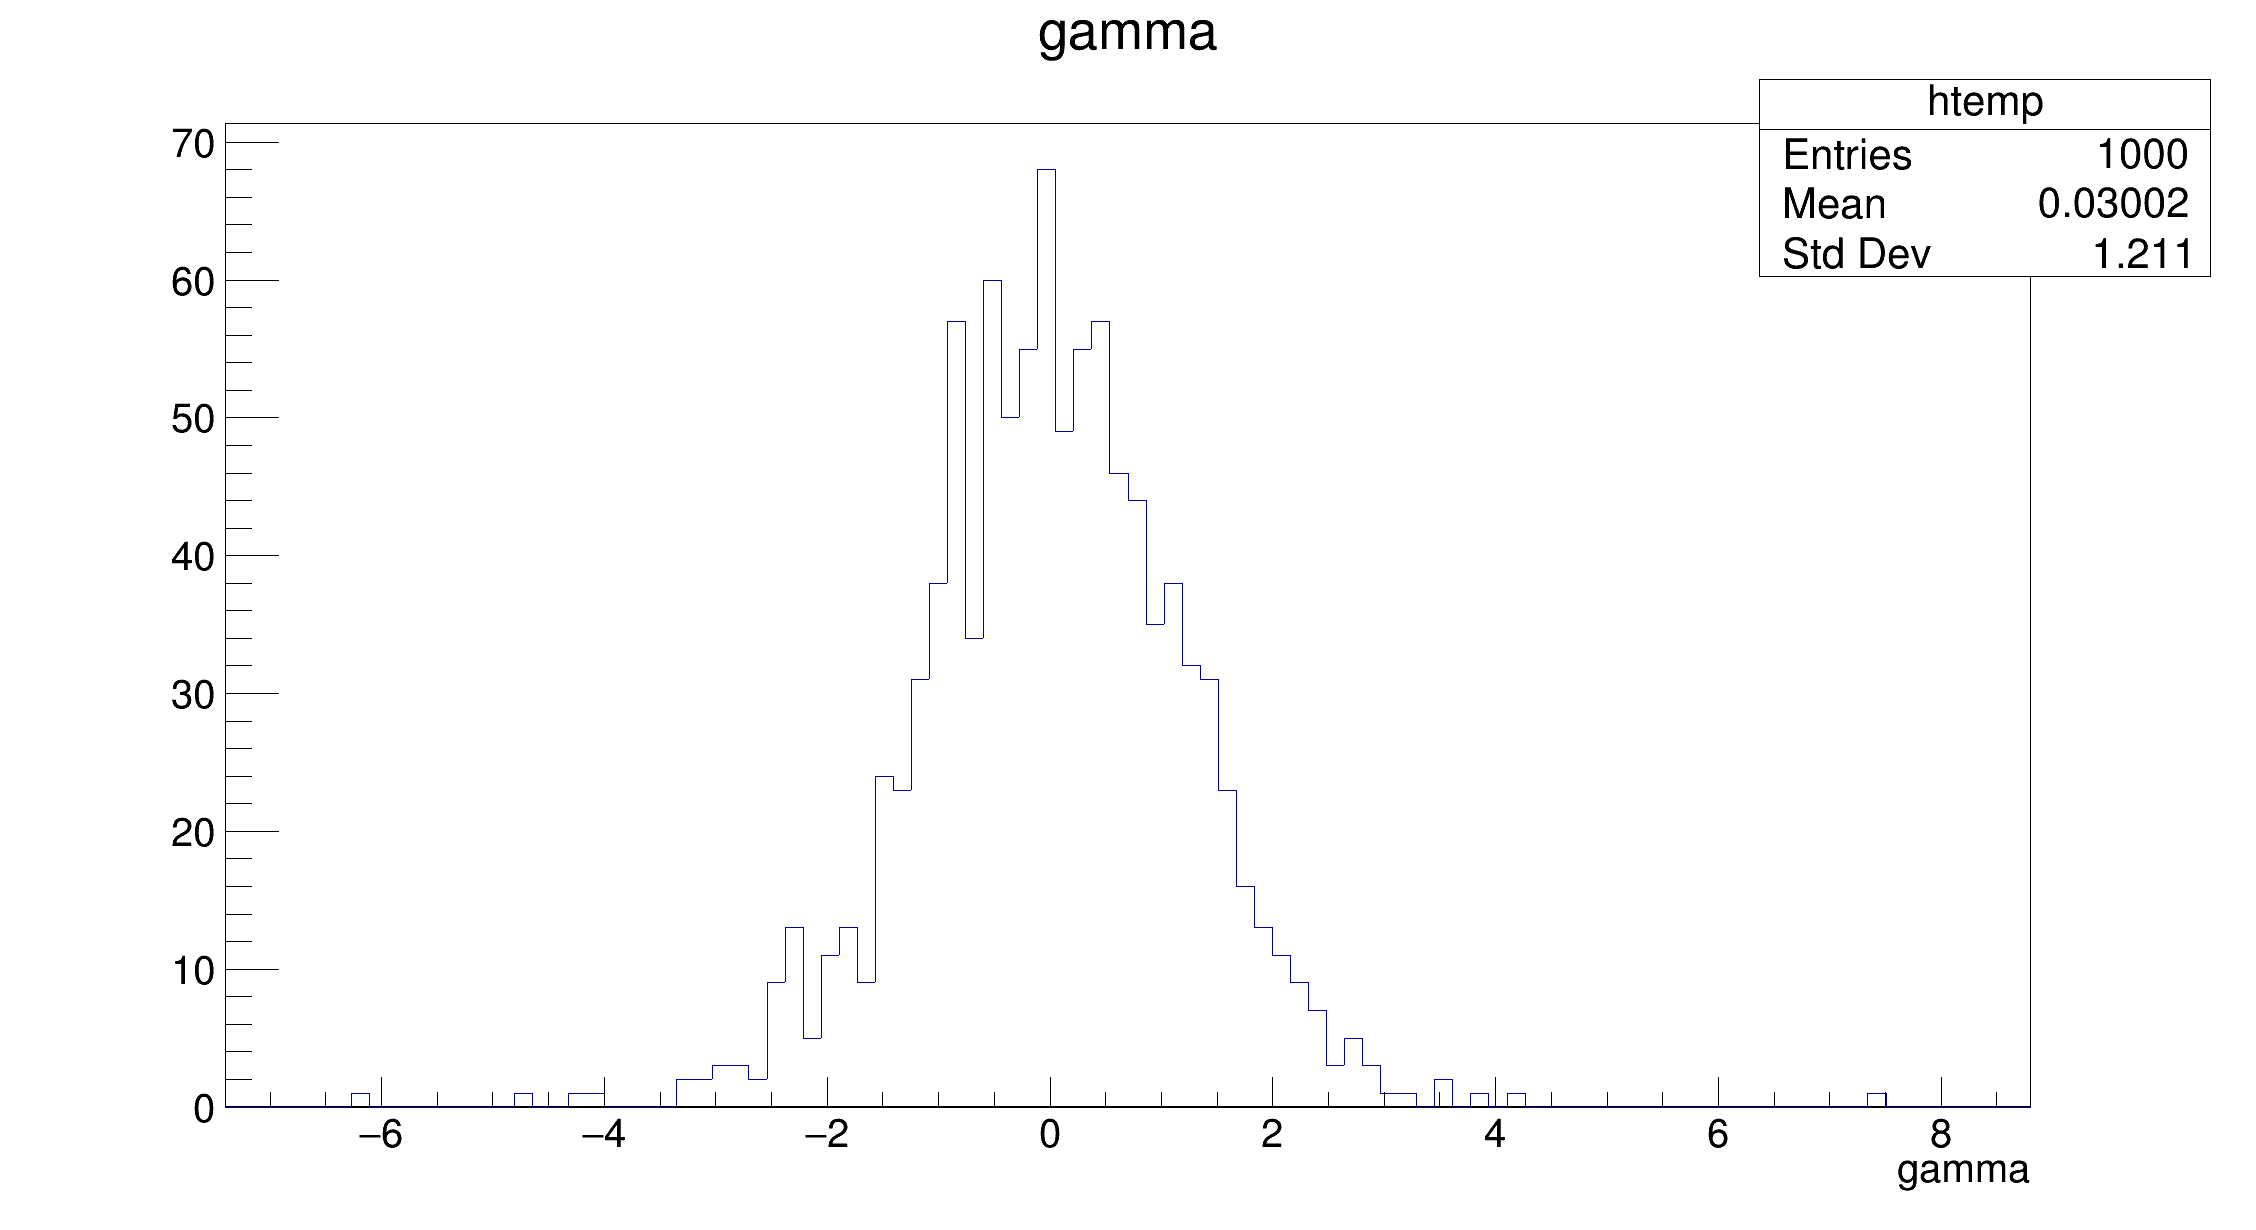
\includegraphics[width = 1.0\textwidth]{SophisticatedPulls/gamma1K1K.png}
      \caption{$\gamma$ pull}
    \end{subfigure}
  \end{figure}
\end{frame}

\begin{frame}{Fitted $\gamma$ values}
  $\gamma$ precision of $21^\circ$
  \begin{figure}
    \centering
    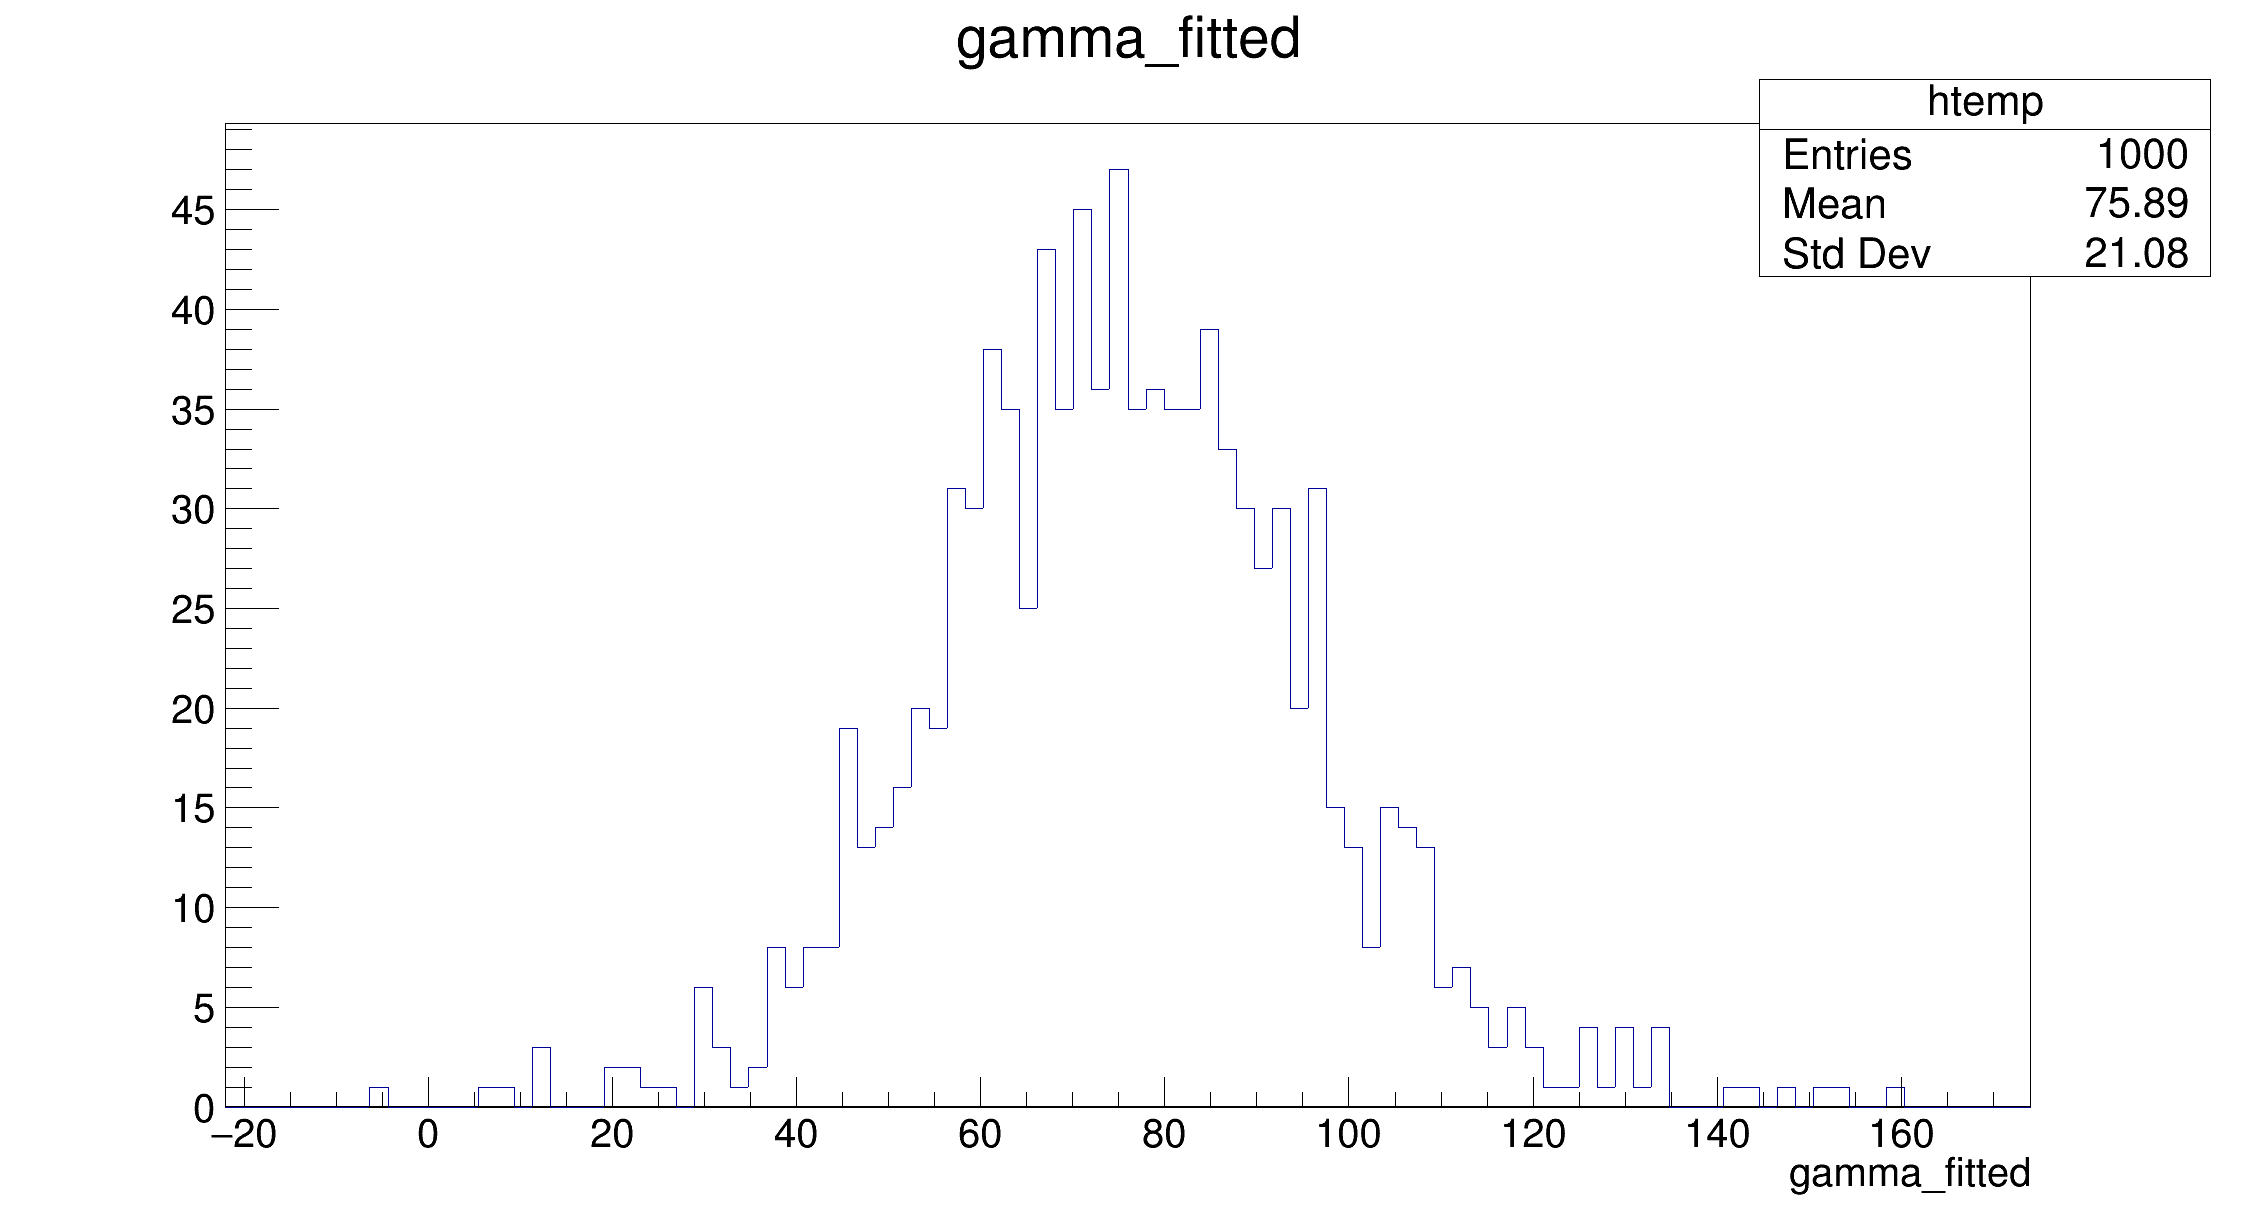
\includegraphics[width = 1.0\textwidth]{SophisticatedPulls/gammafitted1K1K.png}
    \caption{Histogram of fitted $\gamma$ values}
  \end{figure}
\end{frame}

\subsection{Amplitude model binning}
\begin{frame}{Amplitude model binning}
  \begin{itemize}
    \item{Calculate strong phase difference of each event}
    \item{Divide into evenly spaced bins according to their strong phase difference}
    \item{$8$ bins}
  \end{itemize}
\end{frame}

\begin{frame}{Amplitude model binning}
  \begin{figure}
    \centering
    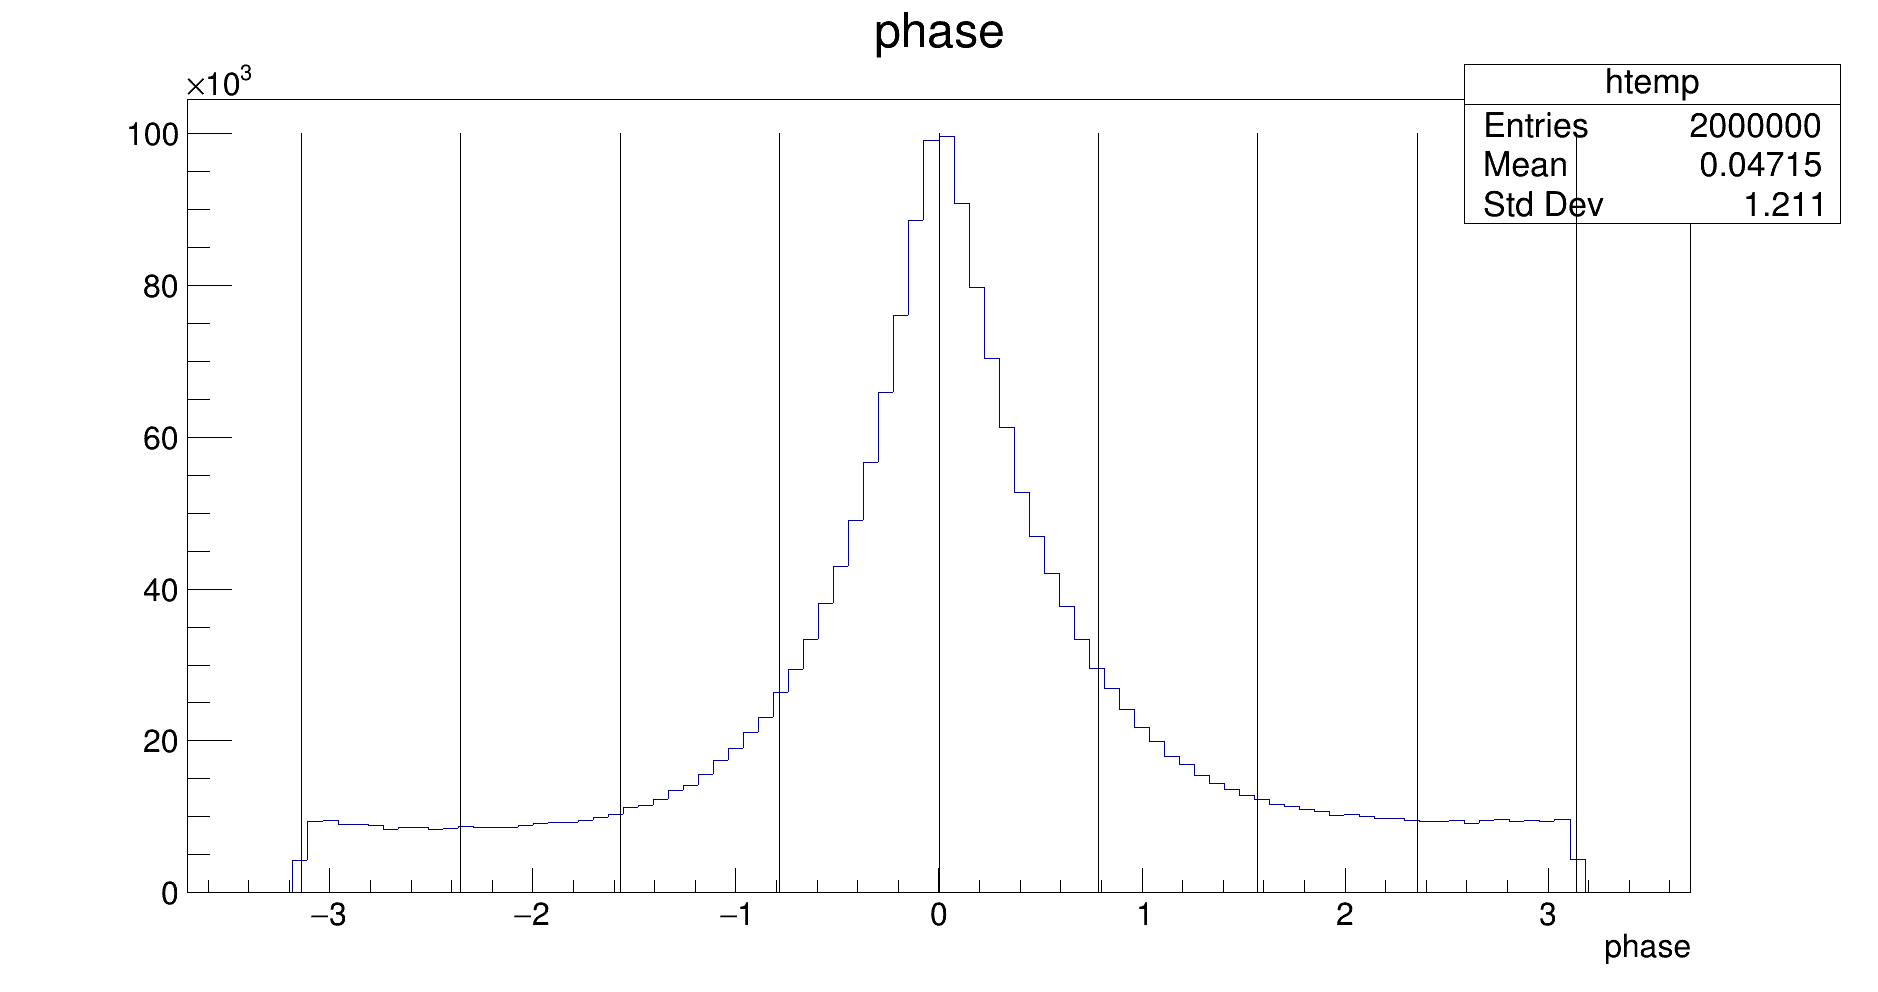
\includegraphics[width = 1.0\textwidth]{EvenStrongPhaseBins.png}
    \caption{Histogram of strong phases, with black lines indicating bins}
  \end{figure}
\end{frame}

\begin{frame}{Pull study with $\SI{2e3}{}$ events}
  \begin{figure}
    \centering
    \vspace{-0.2cm}
    \begin{subfigure}{0.5\textwidth}
      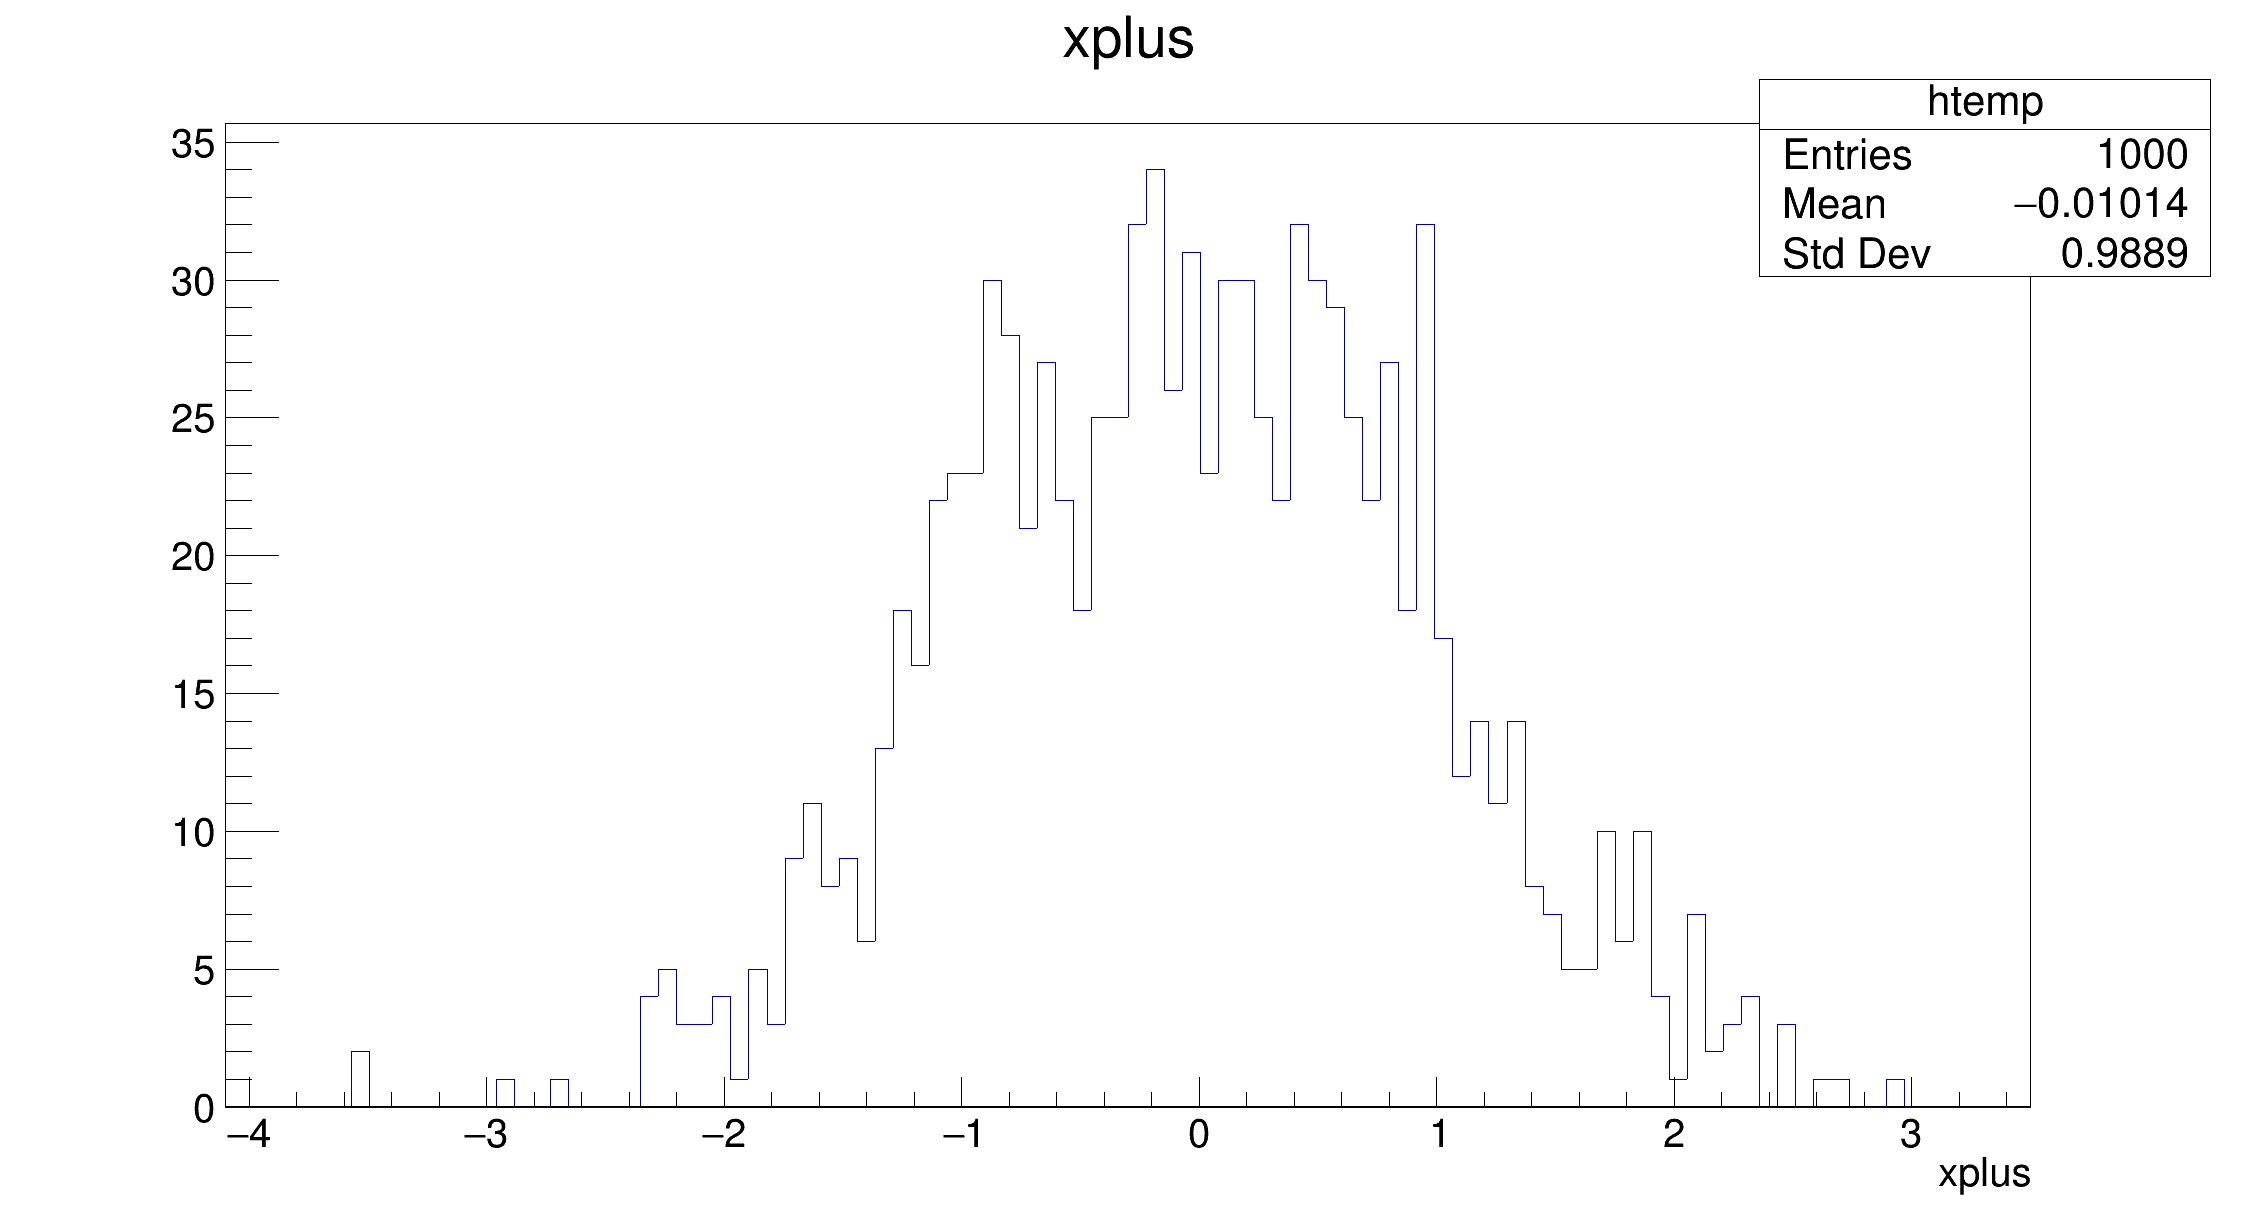
\includegraphics[width = 1.0\textwidth]{AmplitudePulls/xplus1K1K.png}
      \caption{$x_+$ pull}
    \end{subfigure}%
    \begin{subfigure}{0.5\textwidth}
      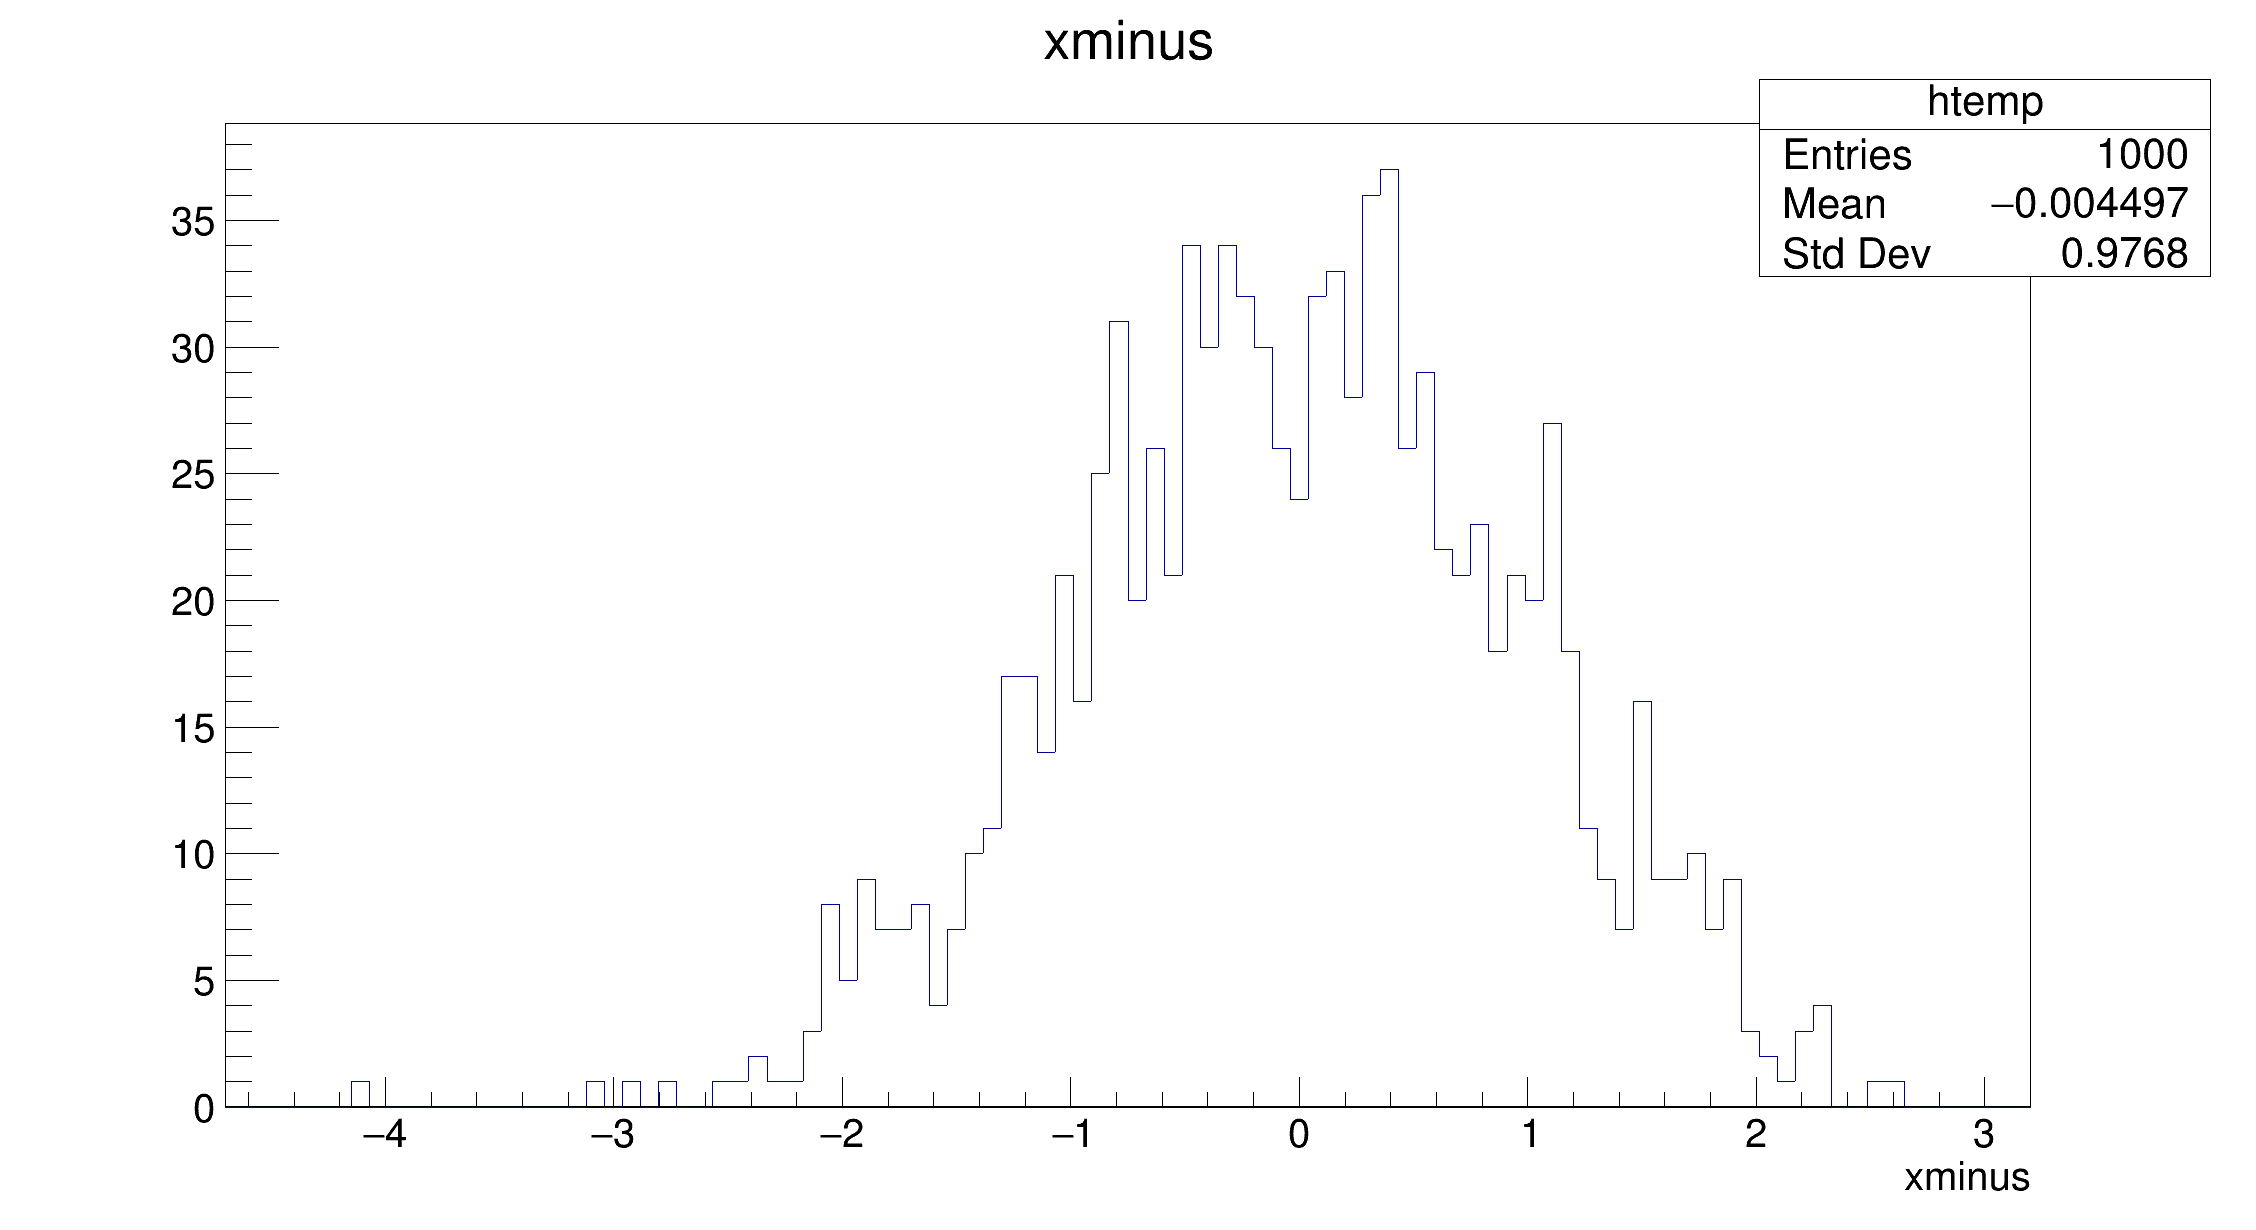
\includegraphics[width = 1.0\textwidth]{AmplitudePulls/xminus1K1K.png}
      \caption{$x_-$ pull}
    \end{subfigure}
    \begin{subfigure}{0.5\textwidth}
      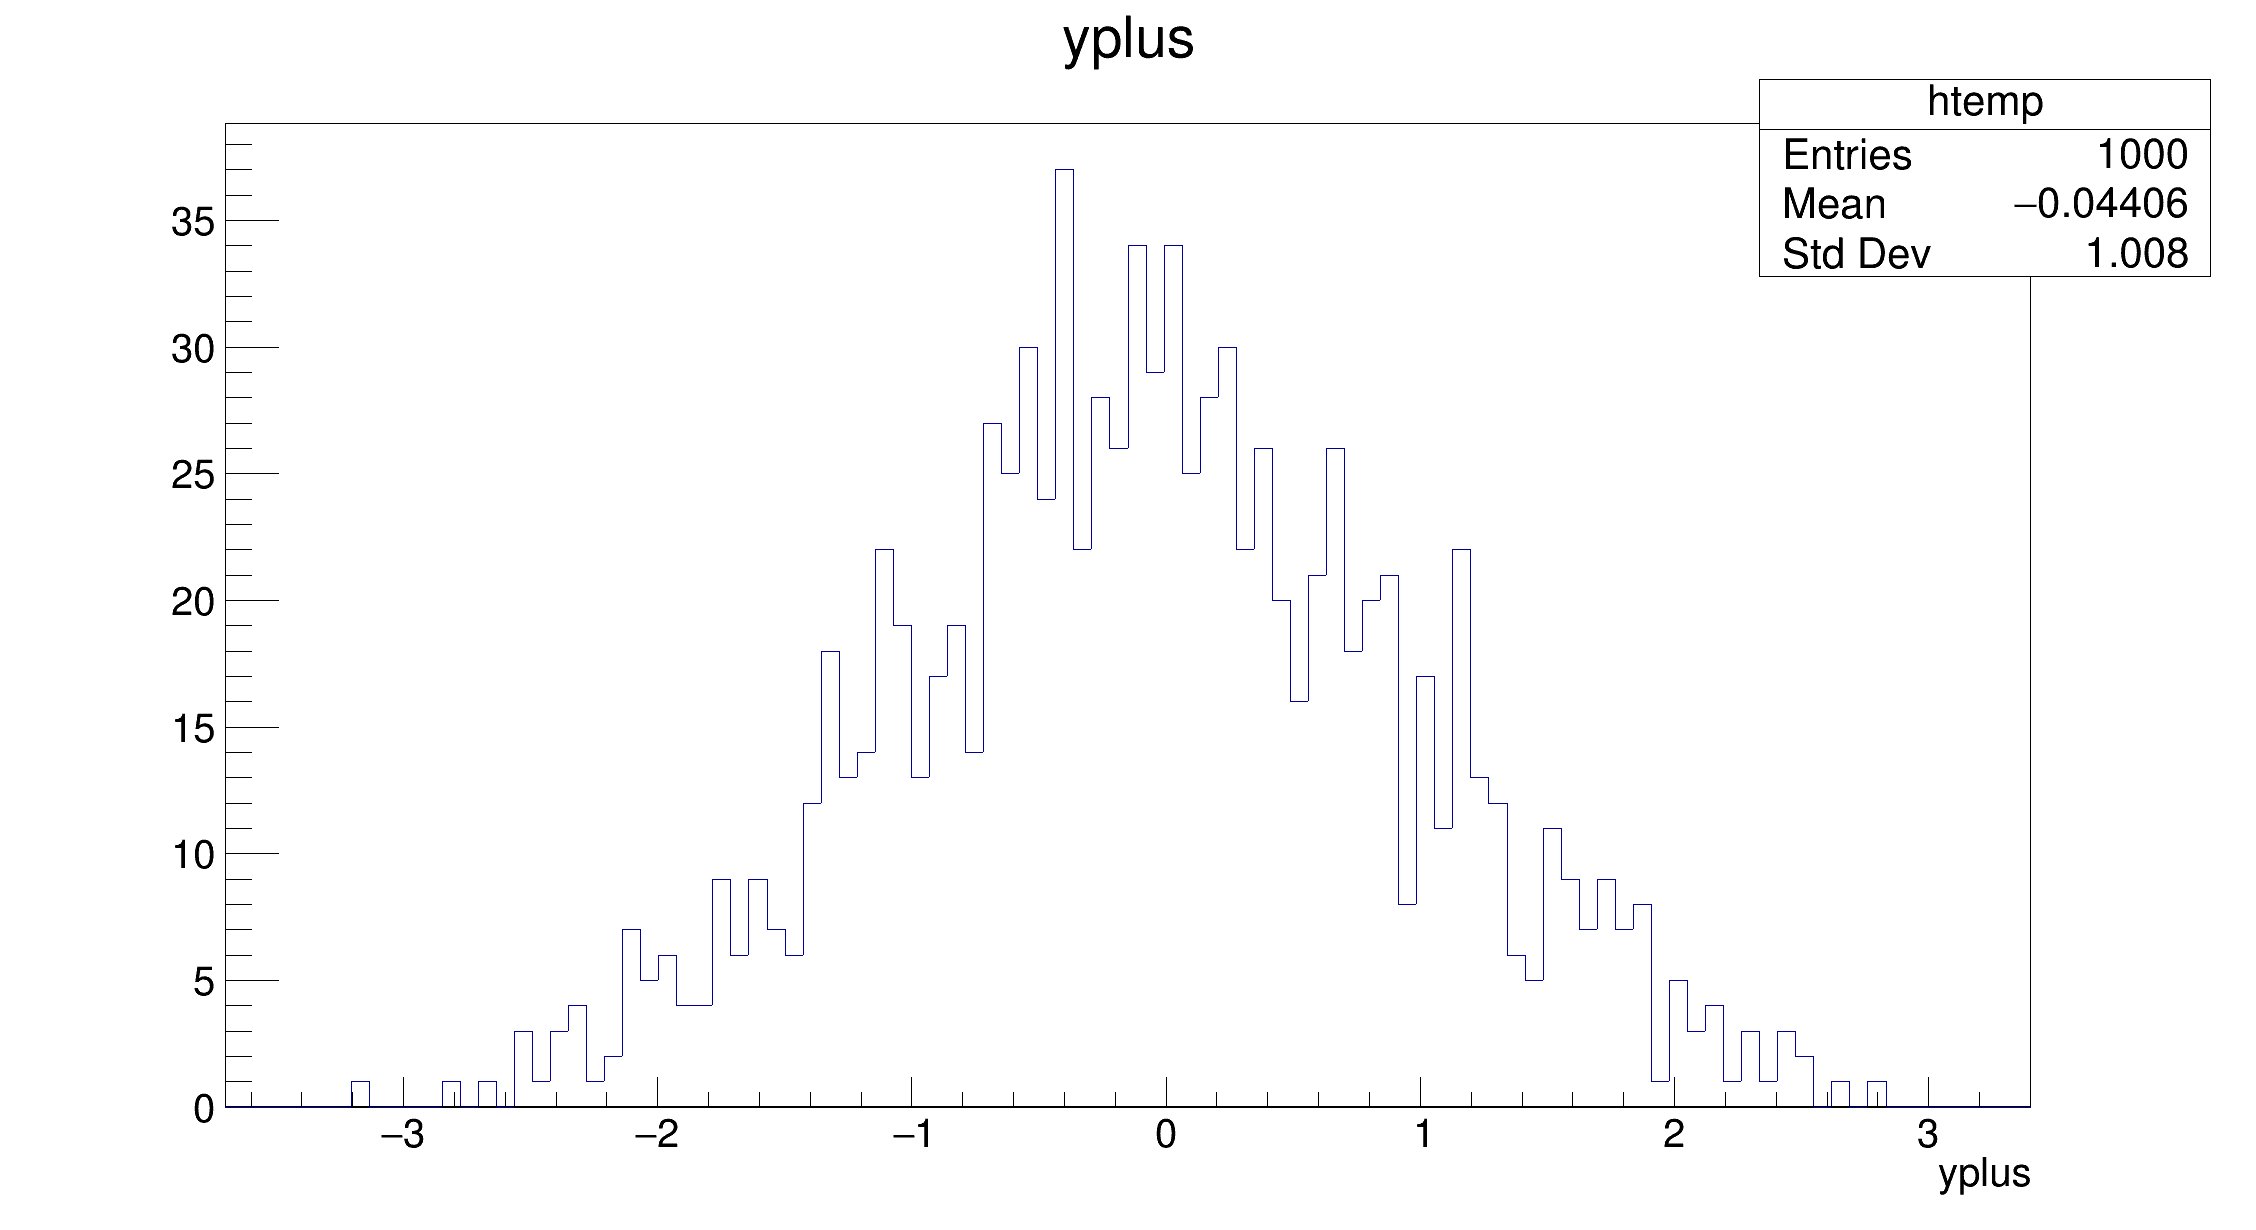
\includegraphics[width = 1.0\textwidth]{AmplitudePulls/yplus1K1K.png}
      \caption{$y_+$ pull}
    \end{subfigure}%
    \begin{subfigure}{0.5\textwidth}
      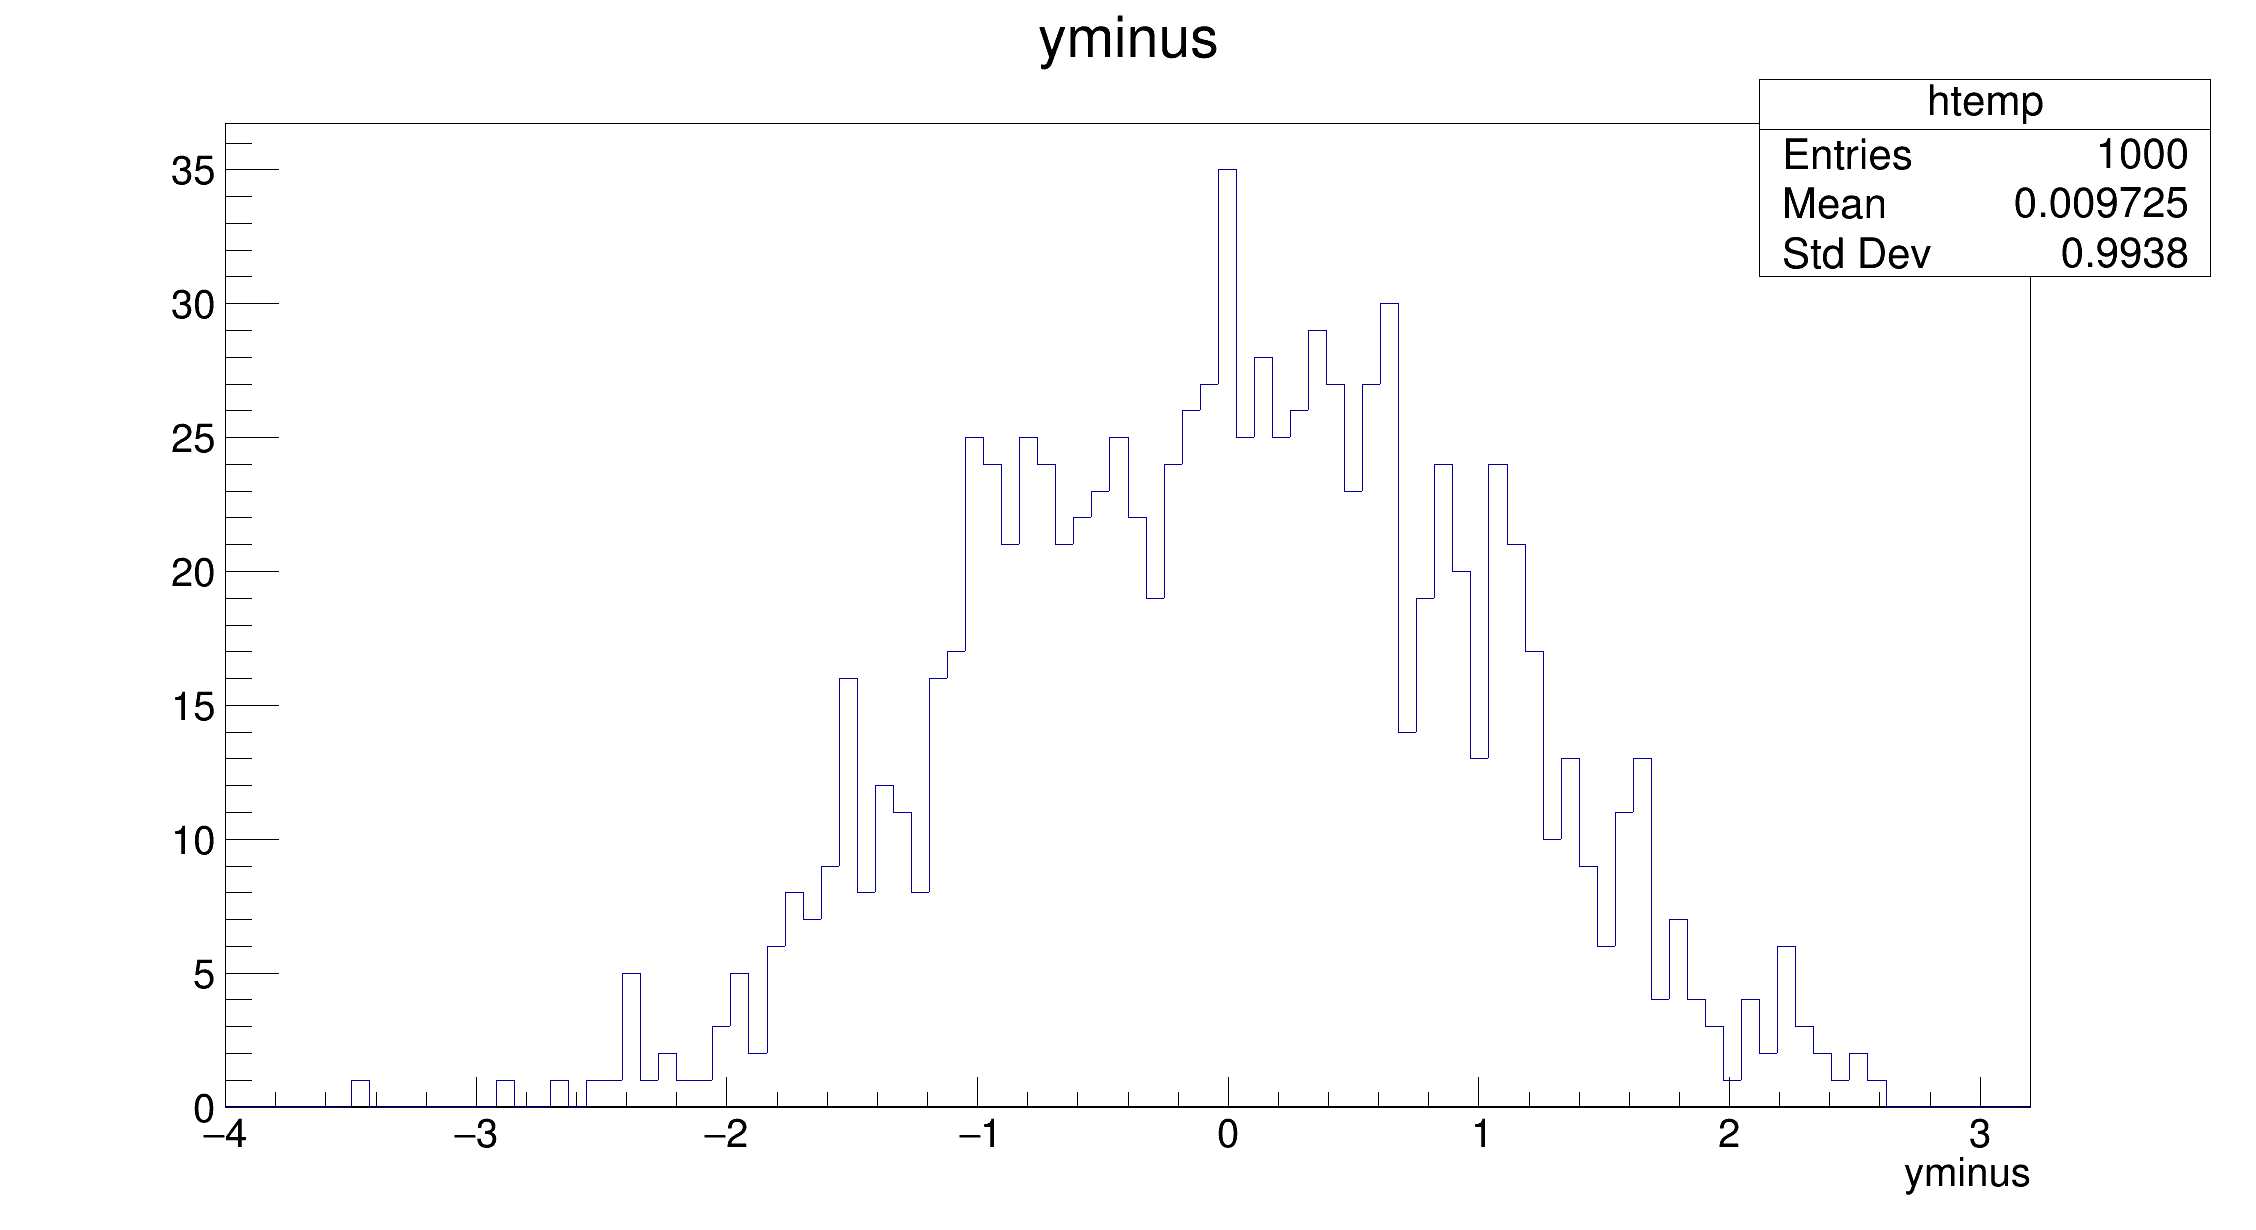
\includegraphics[width = 1.0\textwidth]{AmplitudePulls/yminus1K1K.png}
      \caption{$y_-$ pull}
    \end{subfigure}
  \end{figure}
\end{frame}

\begin{frame}{Pull study with $\SI{2e3}{}$ events}
  \begin{figure}
    \centering
    \vspace{-0.2cm}
    \begin{subfigure}{0.5\textwidth}
      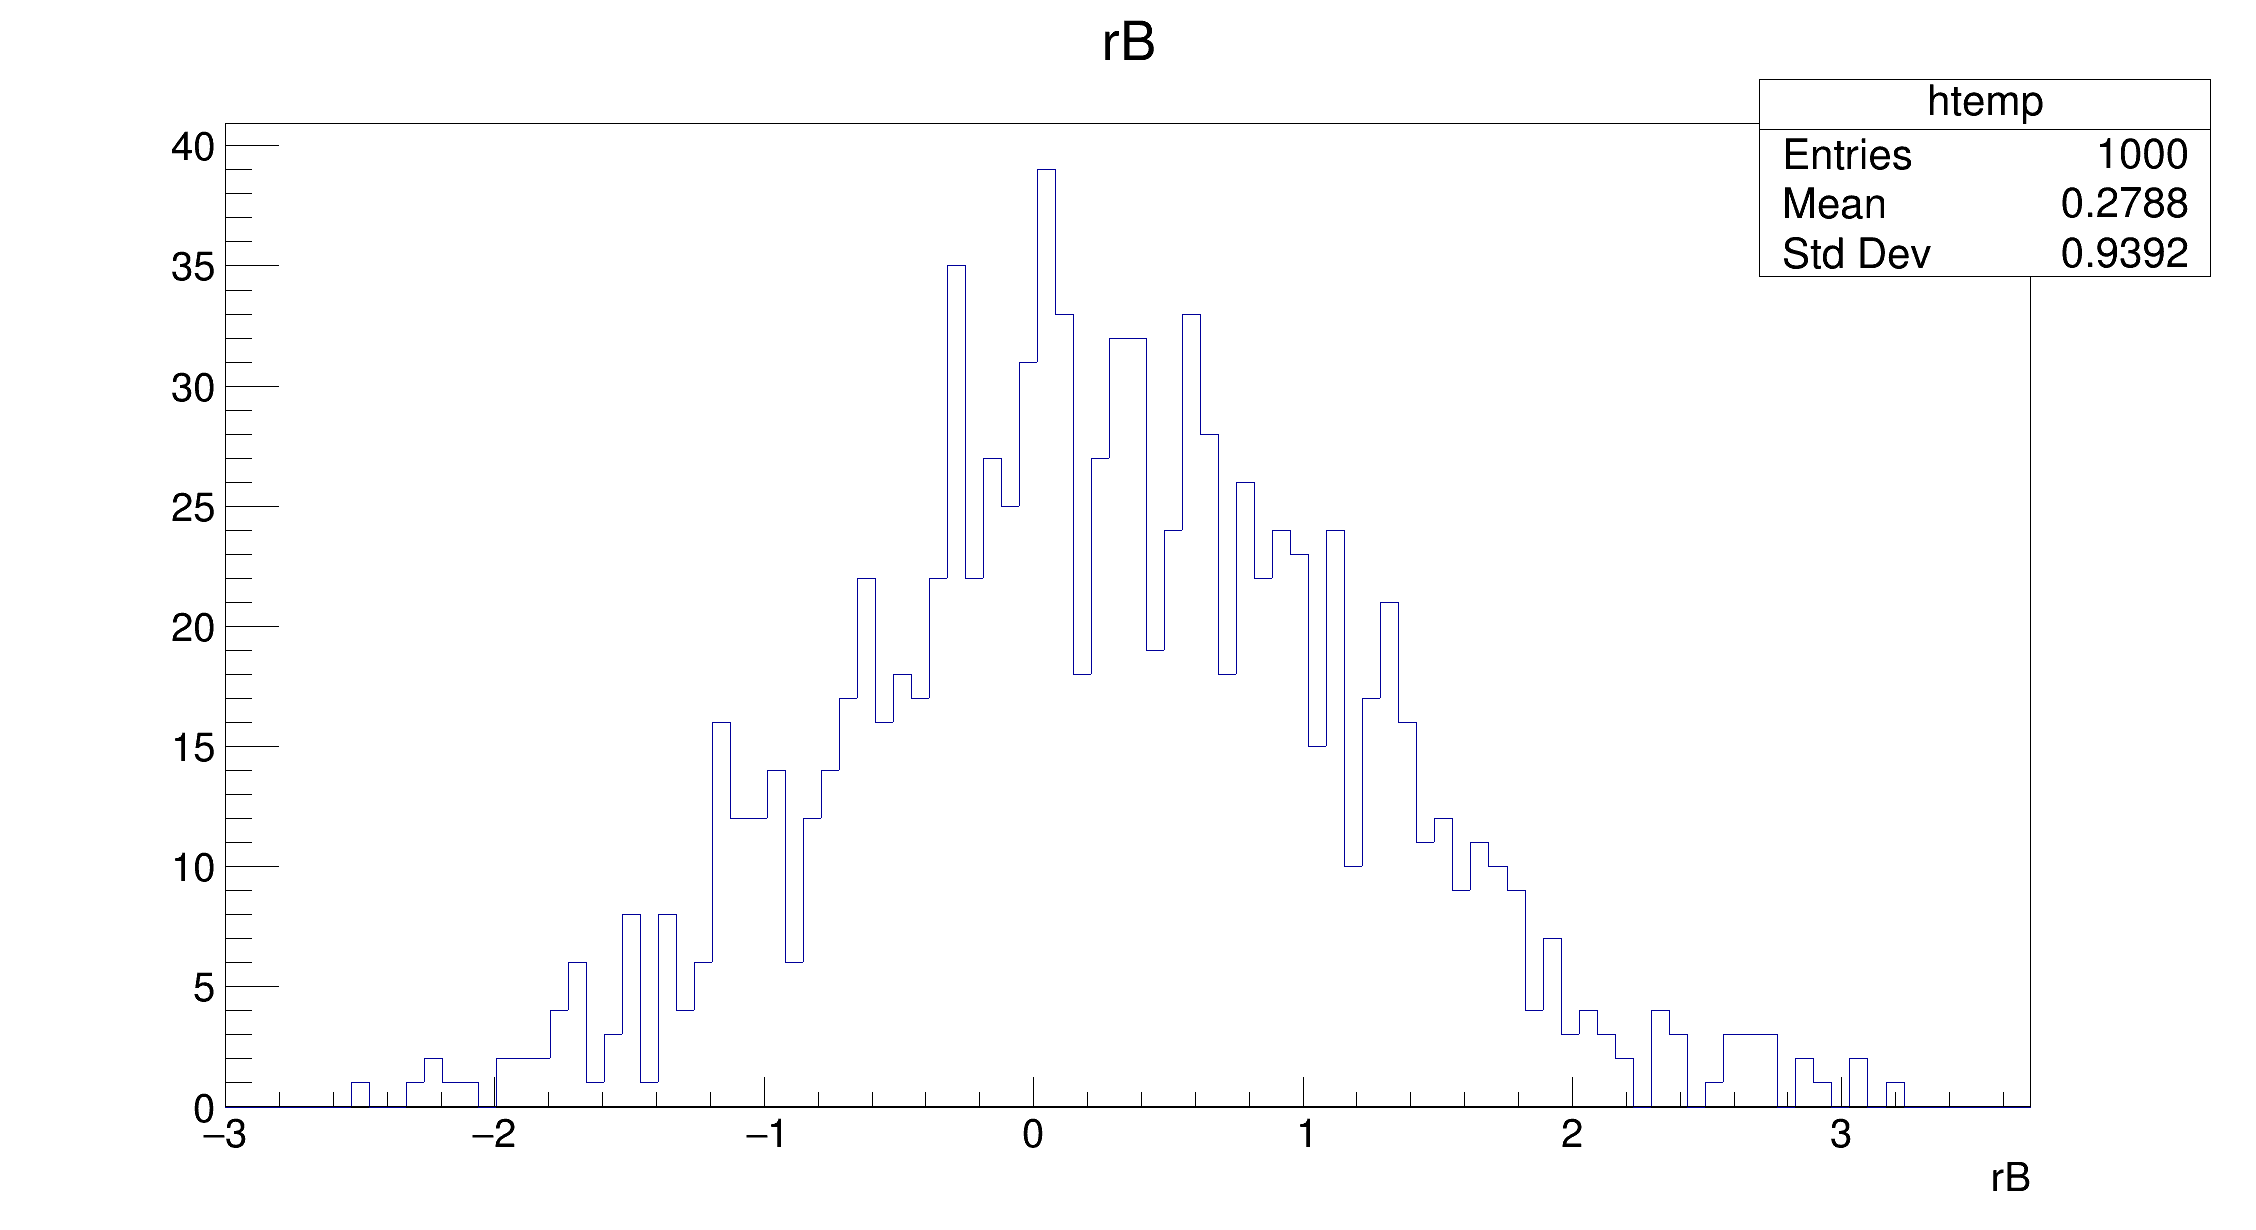
\includegraphics[width = 1.0\textwidth]{AmplitudePulls/rB1K1K.png}
      \caption{$r_B$ pull}
    \end{subfigure}%
    \begin{subfigure}{0.5\textwidth}
      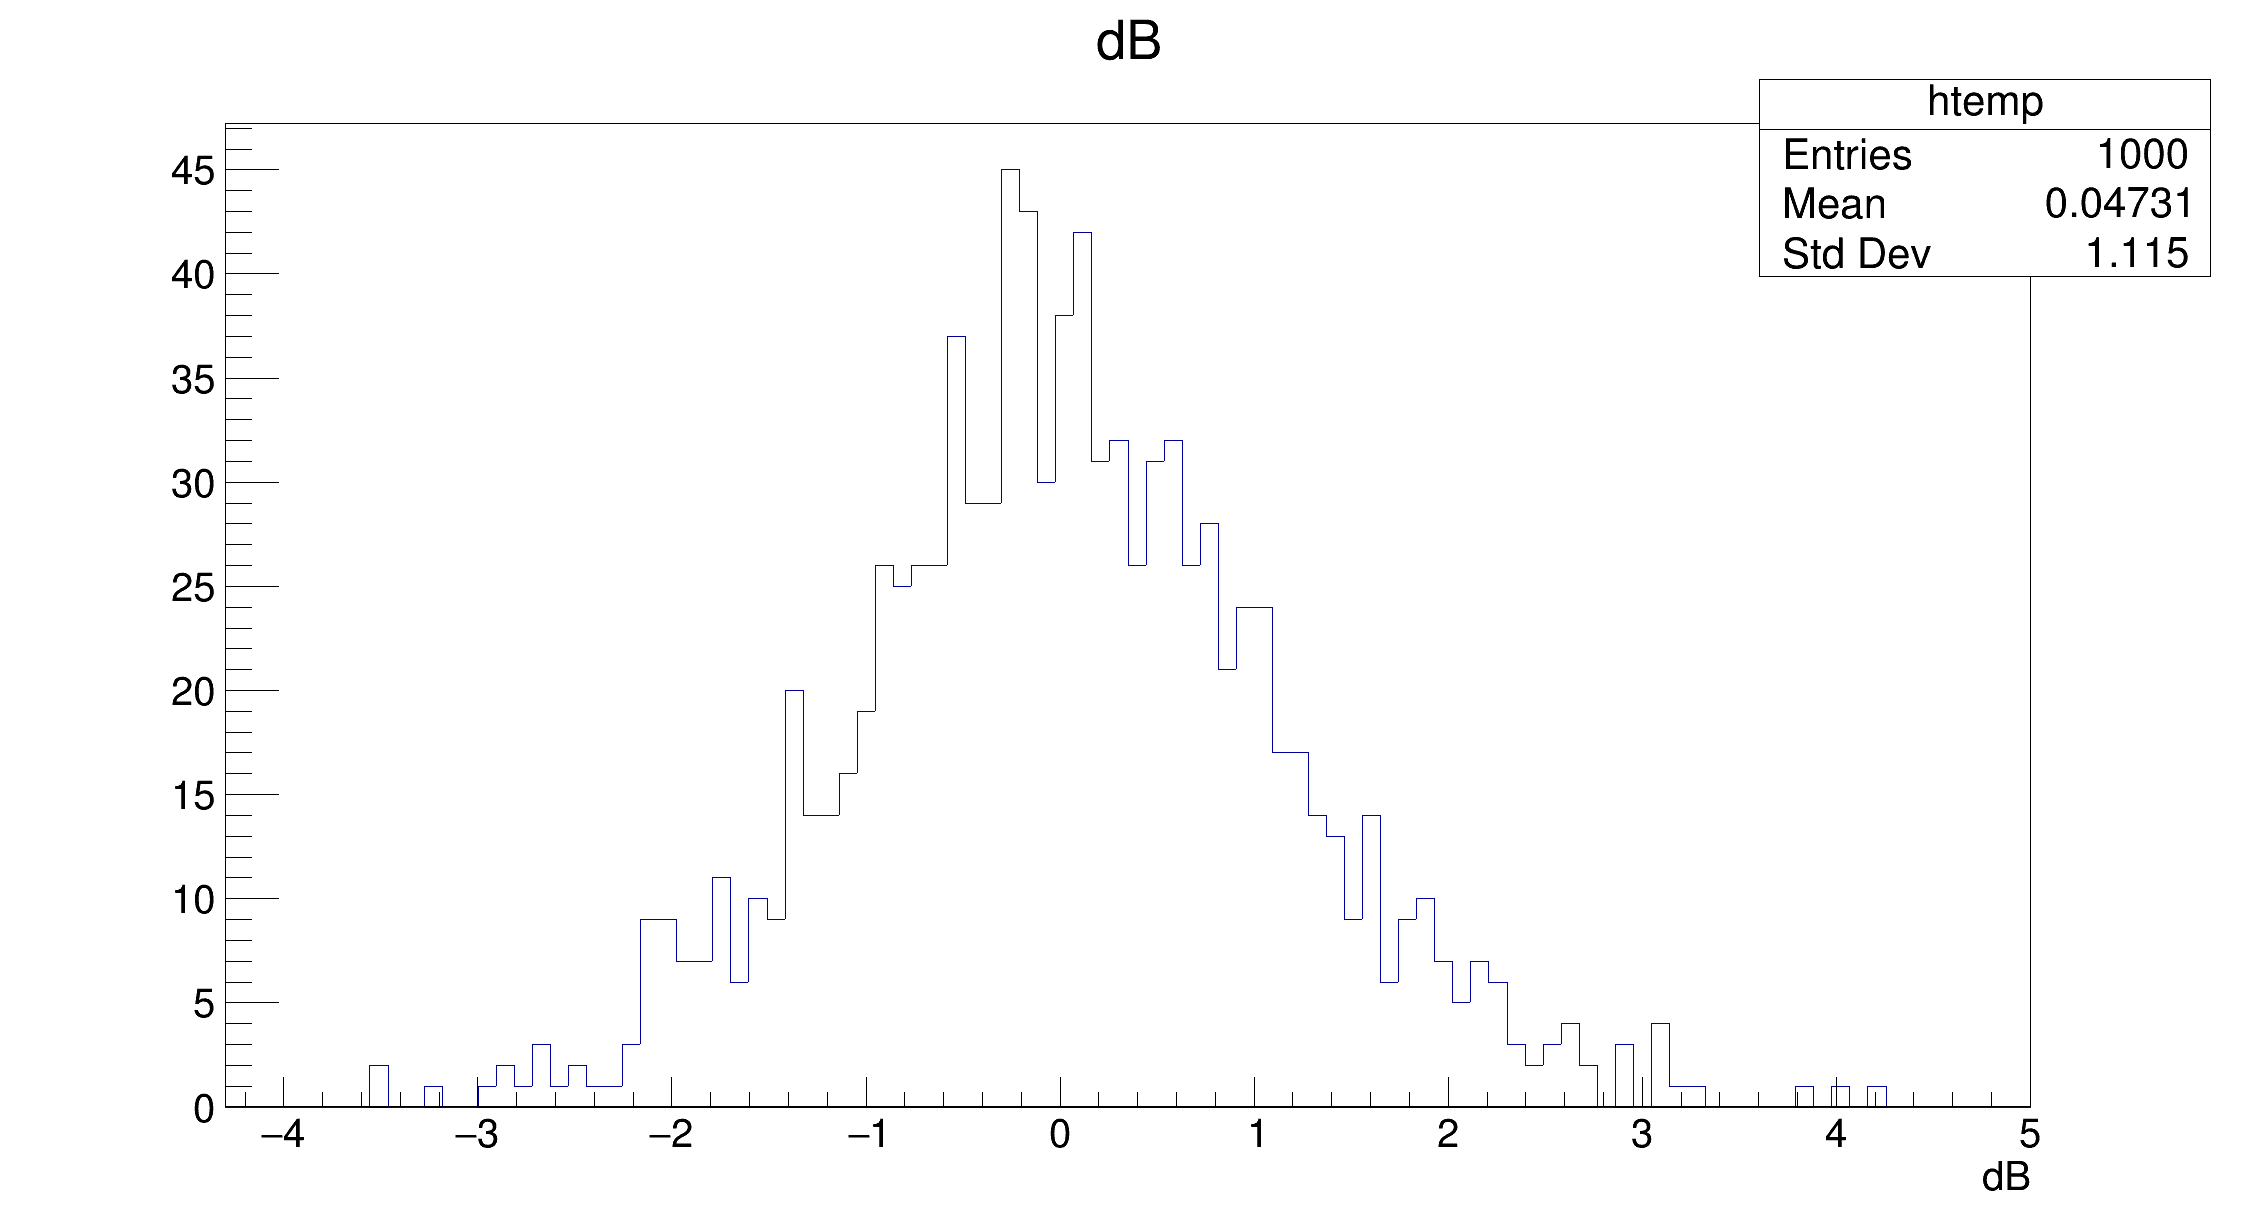
\includegraphics[width = 1.0\textwidth]{AmplitudePulls/dB1K1K.png}
      \caption{$\delta_B$ pull}
    \end{subfigure}
    \begin{subfigure}{0.5\textwidth}
      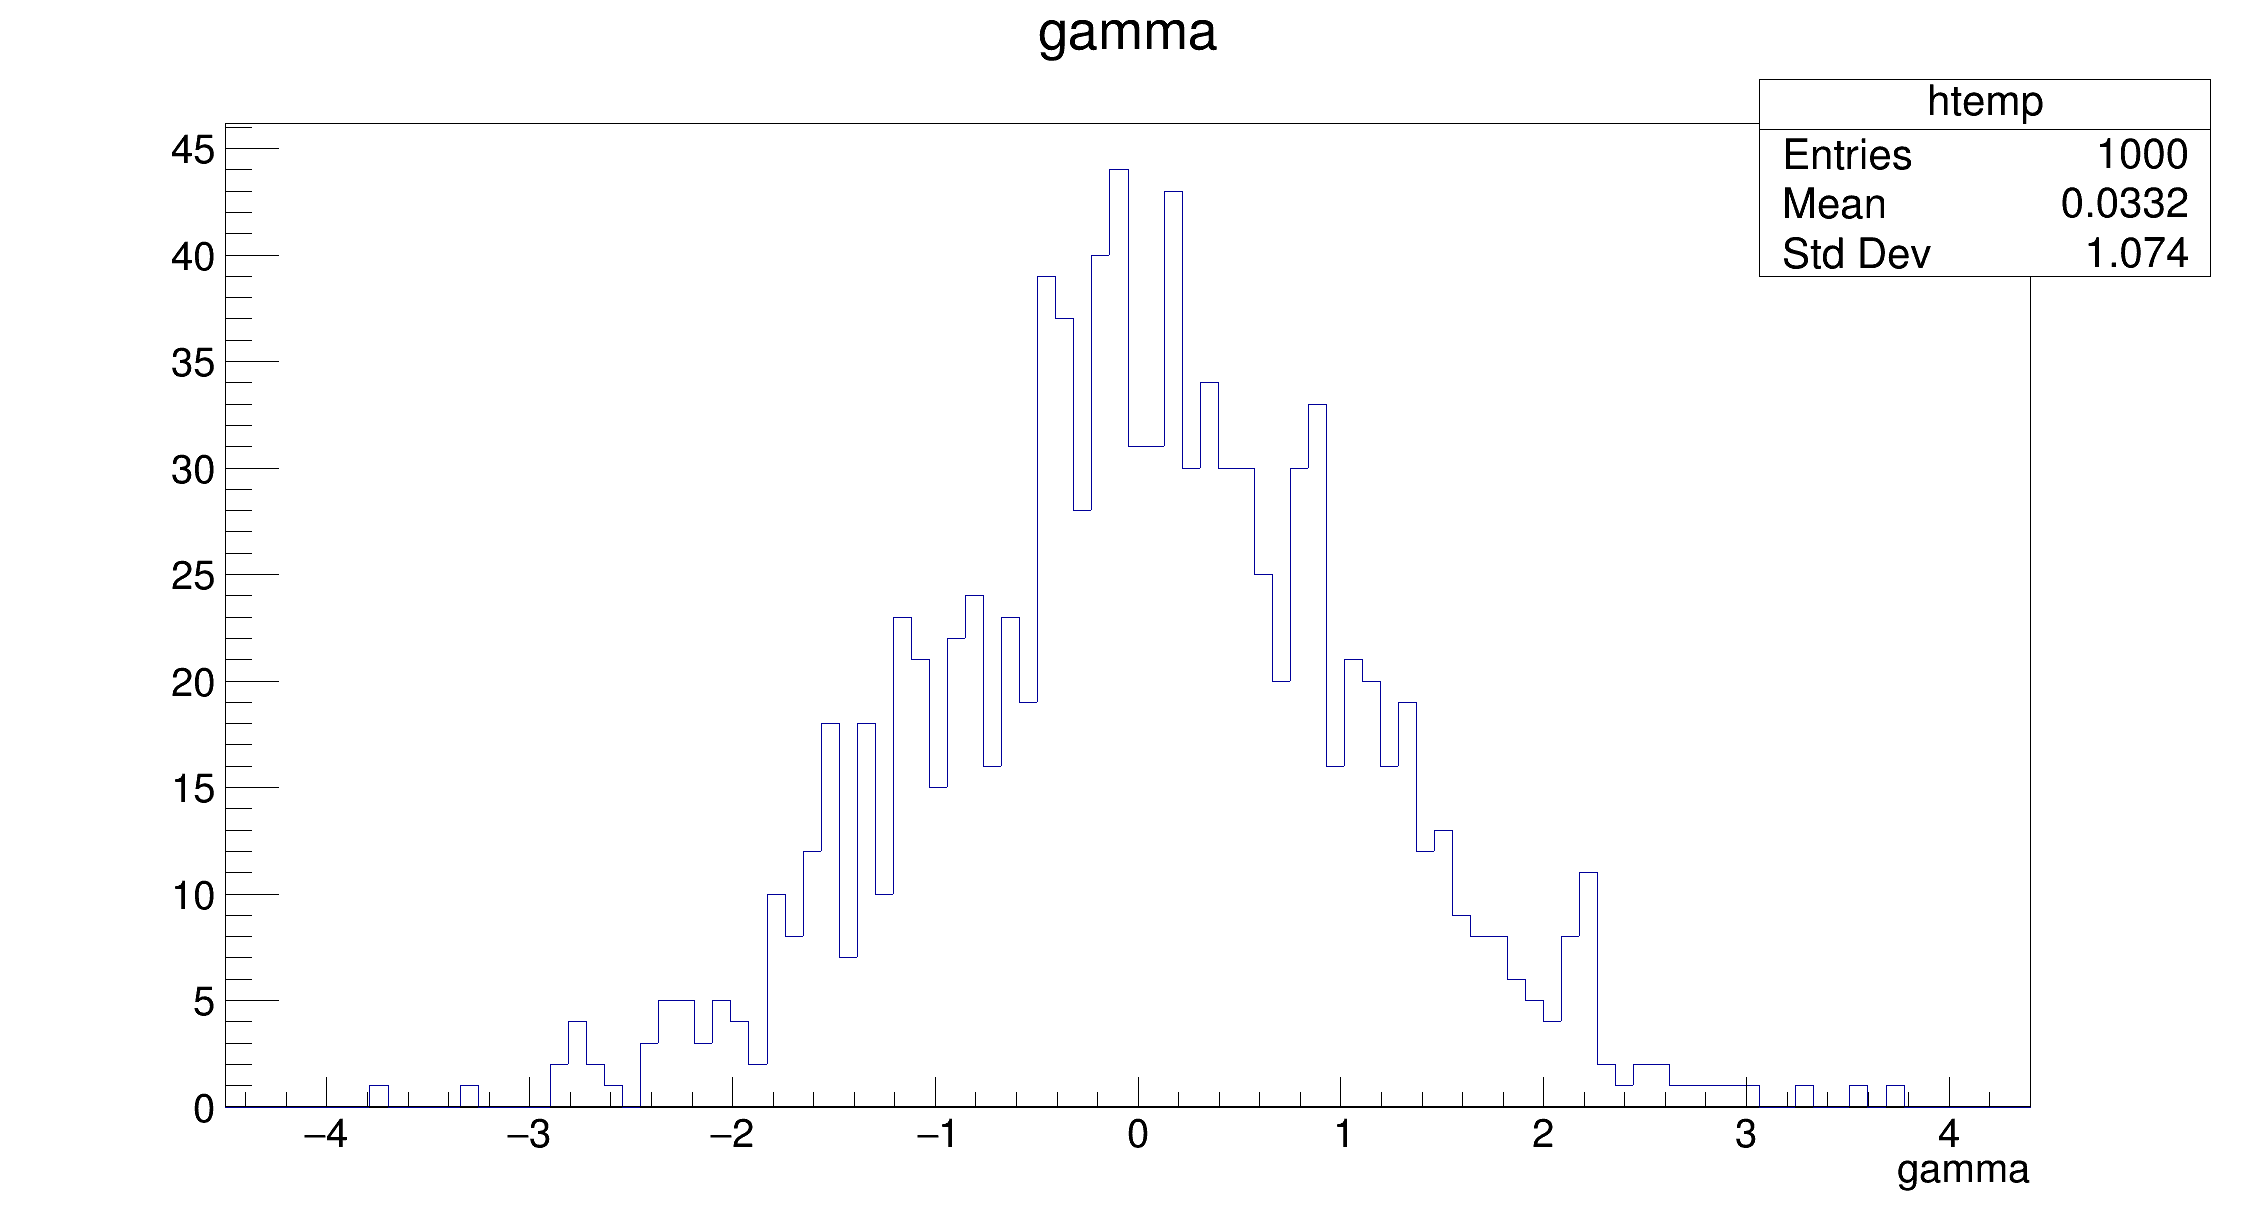
\includegraphics[width = 1.0\textwidth]{AmplitudePulls/gamma1K1K.png}
      \caption{$\gamma$ pull}
    \end{subfigure}
  \end{figure}
\end{frame}

\begin{frame}{Fitted $\gamma$ values}
  $\gamma$ precision of $15.4^\circ$
  \begin{figure}
    \centering
    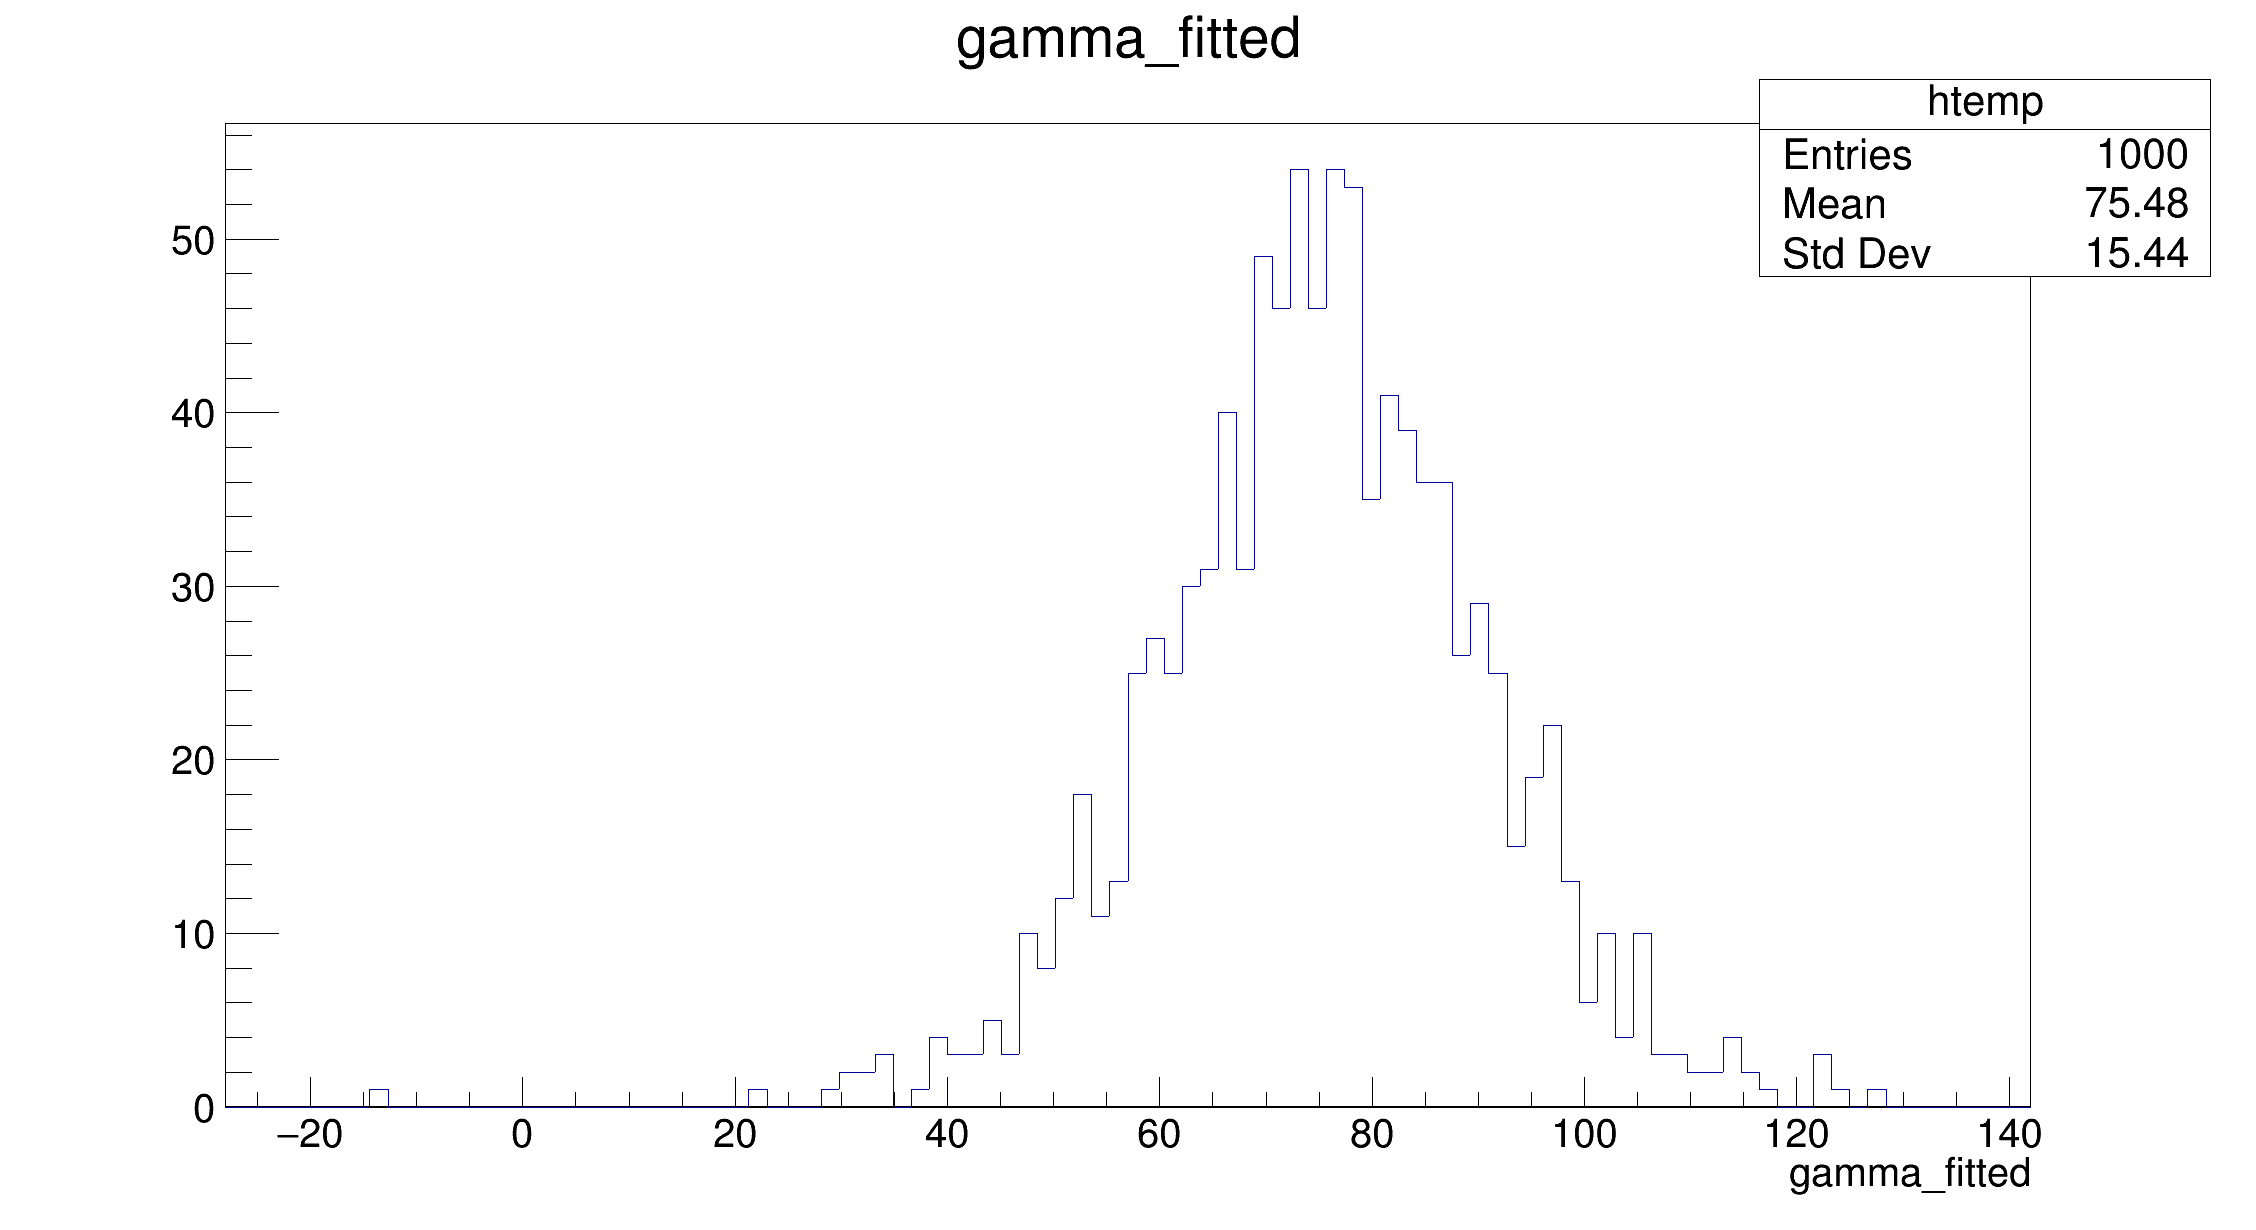
\includegraphics[width = 1.0\textwidth]{AmplitudePulls/gammafitted1K1K.png}
    \caption{Histogram of fitted $\gamma$ values}
  \end{figure}
\end{frame}

\subsection{Amplitude model binning optimized for interference}
\begin{frame}{Maximize interference terms}
  \begin{block}{Event yield in bin $i$}
    $N^-_i = h_{B^-}\Big(K_i + \big(x_-^2 + y_-^2\big)\bar{K_i} + 2\sqrt{K_i\bar{K_i}}\big(x_-c_i + y_-s_i\big)\Big)$
    $N^+_i = h_{B^+}\Big(\bar{K_i} + \big(x_+^2 + y_+^2\big)K_i + 2\sqrt{K_i\bar{K_i}}\big(x_+c_i - y_+s_i\big)\Big)$
  \end{block}
  \begin{itemize}
    \item{Difference of interference terms $\propto\sin(\delta_D + \gamma)$}
    \item{Choose bins such that $\sin(\delta_D + \gamma)$ always has the same sign in each bin}
  \end{itemize}
\end{frame}

\section{Summary}
\begin{frame}{Summary and next steps}
  Summary:
  \begin{itemize}
    \item{Unbinned fit: $11^\circ$ precision with $2000$ events}
    \item{Binned fit: $15.3^\circ$ with $8$ bins}
    \item{Can reach $14.8^\circ$ with $>30$ bins}
  \end{itemize}
  Any suggestions for improving the binning scheme?
\end{frame}

\begin{frame}
  Backup slides
\end{frame}

\end{document}
